% Options for packages loaded elsewhere
\PassOptionsToPackage{unicode}{hyperref}
\PassOptionsToPackage{hyphens}{url}
\PassOptionsToPackage{dvipsnames,svgnames,x11names}{xcolor}
%
\documentclass[
  10pt,
  letterpaper,
]{book}

\usepackage{amsmath,amssymb}
\usepackage{iftex}
\ifPDFTeX
  \usepackage[T1]{fontenc}
  \usepackage[utf8]{inputenc}
  \usepackage{textcomp} % provide euro and other symbols
\else % if luatex or xetex
  \usepackage{unicode-math}
  \defaultfontfeatures{Scale=MatchLowercase}
  \defaultfontfeatures[\rmfamily]{Ligatures=TeX,Scale=1}
\fi
\usepackage{lmodern}
\ifPDFTeX\else  
    % xetex/luatex font selection
\fi
% Use upquote if available, for straight quotes in verbatim environments
\IfFileExists{upquote.sty}{\usepackage{upquote}}{}
\IfFileExists{microtype.sty}{% use microtype if available
  \usepackage[]{microtype}
  \UseMicrotypeSet[protrusion]{basicmath} % disable protrusion for tt fonts
}{}
\makeatletter
\@ifundefined{KOMAClassName}{% if non-KOMA class
  \IfFileExists{parskip.sty}{%
    \usepackage{parskip}
  }{% else
    \setlength{\parindent}{0pt}
    \setlength{\parskip}{6pt plus 2pt minus 1pt}}
}{% if KOMA class
  \KOMAoptions{parskip=half}}
\makeatother
\usepackage{xcolor}
\usepackage[a5paper,top=2.5cm,bottom=1.5cm,left=1.5cm,right=1.5cm]{geometry}
\setlength{\emergencystretch}{3em} % prevent overfull lines
\setcounter{secnumdepth}{5}
% Make \paragraph and \subparagraph free-standing
\makeatletter
\ifx\paragraph\undefined\else
  \let\oldparagraph\paragraph
  \renewcommand{\paragraph}{
    \@ifstar
      \xxxParagraphStar
      \xxxParagraphNoStar
  }
  \newcommand{\xxxParagraphStar}[1]{\oldparagraph*{#1}\mbox{}}
  \newcommand{\xxxParagraphNoStar}[1]{\oldparagraph{#1}\mbox{}}
\fi
\ifx\subparagraph\undefined\else
  \let\oldsubparagraph\subparagraph
  \renewcommand{\subparagraph}{
    \@ifstar
      \xxxSubParagraphStar
      \xxxSubParagraphNoStar
  }
  \newcommand{\xxxSubParagraphStar}[1]{\oldsubparagraph*{#1}\mbox{}}
  \newcommand{\xxxSubParagraphNoStar}[1]{\oldsubparagraph{#1}\mbox{}}
\fi
\makeatother


\providecommand{\tightlist}{%
  \setlength{\itemsep}{0pt}\setlength{\parskip}{0pt}}\usepackage{longtable,booktabs,array}
\usepackage{calc} % for calculating minipage widths
% Correct order of tables after \paragraph or \subparagraph
\usepackage{etoolbox}
\makeatletter
\patchcmd\longtable{\par}{\if@noskipsec\mbox{}\fi\par}{}{}
\makeatother
% Allow footnotes in longtable head/foot
\IfFileExists{footnotehyper.sty}{\usepackage{footnotehyper}}{\usepackage{footnote}}
\makesavenoteenv{longtable}
\usepackage{graphicx}
\makeatletter
\def\maxwidth{\ifdim\Gin@nat@width>\linewidth\linewidth\else\Gin@nat@width\fi}
\def\maxheight{\ifdim\Gin@nat@height>\textheight\textheight\else\Gin@nat@height\fi}
\makeatother
% Scale images if necessary, so that they will not overflow the page
% margins by default, and it is still possible to overwrite the defaults
% using explicit options in \includegraphics[width, height, ...]{}
\setkeys{Gin}{width=\maxwidth,height=\maxheight,keepaspectratio}
% Set default figure placement to htbp
\makeatletter
\def\fps@figure{htbp}
\makeatother
% definitions for citeproc citations
\NewDocumentCommand\citeproctext{}{}
\NewDocumentCommand\citeproc{mm}{%
  \begingroup\def\citeproctext{#2}\cite{#1}\endgroup}
\makeatletter
 % allow citations to break across lines
 \let\@cite@ofmt\@firstofone
 % avoid brackets around text for \cite:
 \def\@biblabel#1{}
 \def\@cite#1#2{{#1\if@tempswa , #2\fi}}
\makeatother
\newlength{\cslhangindent}
\setlength{\cslhangindent}{1.5em}
\newlength{\csllabelwidth}
\setlength{\csllabelwidth}{3em}
\newenvironment{CSLReferences}[2] % #1 hanging-indent, #2 entry-spacing
 {\begin{list}{}{%
  \setlength{\itemindent}{0pt}
  \setlength{\leftmargin}{0pt}
  \setlength{\parsep}{0pt}
  % turn on hanging indent if param 1 is 1
  \ifodd #1
   \setlength{\leftmargin}{\cslhangindent}
   \setlength{\itemindent}{-1\cslhangindent}
  \fi
  % set entry spacing
  \setlength{\itemsep}{#2\baselineskip}}}
 {\end{list}}
\usepackage{calc}
\newcommand{\CSLBlock}[1]{\hfill\break\parbox[t]{\linewidth}{\strut\ignorespaces#1\strut}}
\newcommand{\CSLLeftMargin}[1]{\parbox[t]{\csllabelwidth}{\strut#1\strut}}
\newcommand{\CSLRightInline}[1]{\parbox[t]{\linewidth - \csllabelwidth}{\strut#1\strut}}
\newcommand{\CSLIndent}[1]{\hspace{\cslhangindent}#1}

% Cargar fuentes y paquetes de estilo
\usepackage{fontspec}
\setmainfont{IBM Plex Serif}          % Fuente principal para el texto del libro
\setsansfont{IBM Plex Sans}           % Fuente sans-serif para los títulos
\setmonofont{IBM Plex Mono}           % Fuente para código
\usepackage{xcolor}
\definecolor{highlight}{RGB}{29, 120, 200} % Color para enlaces

% Paquete para soporte de idiomas
\usepackage{polyglossia}
\setmainlanguage{spanish}  % Define español como idioma principal
\usepackage{microtype}      % Mejorar la legibilidad

% Paquete para la personalización del título
\usepackage{titling}

% Encabezados y pies de página elegantes
\usepackage{fancyhdr}
\pagestyle{fancy}
\fancyhf{}
\fancyhead[LE,RO]{\thepage}  % Número de página en las esquinas
\fancyhead[RE]{\nouppercase{\leftmark}}  % Nombre del capítulo
\fancyhead[LO]{\nouppercase{\rightmark}} % Nombre de la sección
\fancyfoot[C]{\thepage}
\makeatletter
\@ifpackageloaded{bookmark}{}{\usepackage{bookmark}}
\makeatother
\makeatletter
\@ifpackageloaded{caption}{}{\usepackage{caption}}
\AtBeginDocument{%
\ifdefined\contentsname
  \renewcommand*\contentsname{Table of contents}
\else
  \newcommand\contentsname{Table of contents}
\fi
\ifdefined\listfigurename
  \renewcommand*\listfigurename{List of Figures}
\else
  \newcommand\listfigurename{List of Figures}
\fi
\ifdefined\listtablename
  \renewcommand*\listtablename{List of Tables}
\else
  \newcommand\listtablename{List of Tables}
\fi
\ifdefined\figurename
  \renewcommand*\figurename{Figure}
\else
  \newcommand\figurename{Figure}
\fi
\ifdefined\tablename
  \renewcommand*\tablename{Table}
\else
  \newcommand\tablename{Table}
\fi
}
\@ifpackageloaded{float}{}{\usepackage{float}}
\floatstyle{ruled}
\@ifundefined{c@chapter}{\newfloat{codelisting}{h}{lop}}{\newfloat{codelisting}{h}{lop}[chapter]}
\floatname{codelisting}{Listing}
\newcommand*\listoflistings{\listof{codelisting}{List of Listings}}
\makeatother
\makeatletter
\makeatother
\makeatletter
\@ifpackageloaded{caption}{}{\usepackage{caption}}
\@ifpackageloaded{subcaption}{}{\usepackage{subcaption}}
\makeatother

\ifLuaTeX
  \usepackage{selnolig}  % disable illegal ligatures
\fi
\usepackage{bookmark}

\IfFileExists{xurl.sty}{\usepackage{xurl}}{} % add URL line breaks if available
\urlstyle{same} % disable monospaced font for URLs
\hypersetup{
  pdftitle={iabookMaquiloca},
  pdfauthor={Javier Flores},
  colorlinks=true,
  linkcolor={highlight},
  filecolor={Maroon},
  citecolor={Blue},
  urlcolor={highlight},
  pdfcreator={LaTeX via pandoc}}


\title{iabookMaquiloca}
\author{Javier Flores}
\date{2024-09-10}

\begin{document}
\frontmatter
\maketitle

% Página de título con estilo moderno
\pretitle{\begin{center}\Huge\sffamily\bfseries}
\posttitle{\end{center}}
\preauthor{\begin{center}\large\sffamily}
\postauthor{\end{center}}
\predate{\begin{center}\large}
\postdate{\end{center}\vspace{2cm}}
\maketitle

\renewcommand*\contentsname{Table of contents}
{
\hypersetup{linkcolor=}
\setcounter{tocdepth}{1}
\tableofcontents
}

\mainmatter
\bookmarksetup{startatroot}

\chapter*{Preface El Futuro se Escribe en la
Frontera}\label{preface-el-futuro-se-escribe-en-la-frontera}
\addcontentsline{toc}{chapter}{Preface El Futuro se Escribe en la
Frontera}

\markboth{Preface El Futuro se Escribe en la Frontera}{Preface El Futuro
se Escribe en la Frontera}

\section*{Introducción}\label{introducciuxf3n}
\addcontentsline{toc}{section}{Introducción}

\markright{Introducción}

Ciudad Juárez, crisol de culturas y encrucijada de industrias, se
encuentra en el umbral de una nueva era. La inteligencia artificial, esa
fuerza transformadora que redefine los límites de lo posible, está
llegando a las entrañas de la maquiladora, prometiendo una revolución
silenciosa pero profunda.

Este libro es un viaje a través de esa revolución. Exploraremos cómo la
IA está cambiando la forma en que se produce, se innova y se compite en
la frontera. Desde los robots que comparten espacio con los trabajadores
en la línea de montaje, hasta los algoritmos que predicen la demanda del
mercado con una precisión asombrosa, la IA está dejando su huella en
cada rincón de la industria.

Pero este libro no es solo sobre tecnología. Es sobre las personas que
dan vida a la maquiladora, los hombres y mujeres cuya labor diaria
construye el futuro de Juárez. Es sobre cómo la IA puede empoderarlos,
liberándolos de tareas repetitivas y peligrosas, y permitiéndoles
desarrollar todo su potencial creativo.

Y es, sobre todo, un homenaje a Ciudad Juárez, mi ciudad, esa tierra
indomable que siempre ha sabido reinventarse frente a la adversidad. Que
este libro sea un testimonio de su espíritu innovador, de su capacidad
para abrazar el cambio y forjar un futuro más próspero para todos.

\section*{Dedicatoria}\label{dedicatoria}
\addcontentsline{toc}{section}{Dedicatoria}

\markright{Dedicatoria}

A Ciudad Juárez, mi hogar, mi inspiración. A su gente trabajadora y
resiliente, que día a día construye un futuro mejor. Y a la memoria de
mi novia Alejandra Mendez, quien siempre creyó en mí y en el potencial
de esta ciudad.

\section*{Agradecimientos}\label{agradecimientos}
\addcontentsline{toc}{section}{Agradecimientos}

\markright{Agradecimientos}

Al equipo del IACenter, especialmente a Eduardo Castillo y Joam Ricon,
por su apoyo incondicional y su visión compartida. A todos los expertos
y profesionales que contribuyeron con sus conocimientos y experiencias a
este libro. Y a mi familia y amigos, por su amor y aliento constantes.

\section*{Público Objetivo}\label{puxfablico-objetivo}
\addcontentsline{toc}{section}{Público Objetivo}

\markright{Público Objetivo}

Este libro está dirigido a dos grandes grupos: los que están al mando en
la industria maquiladora de Ciudad Juárez, como los gerentes y
administradores, y también a los estudiantes que están empezando a
meterse en este mundo. ¿Por qué? Pues porque aquí vas a encontrar la
mezcla perfecta entre lo que necesitas saber para mantener tu maquila en
la cima y una introducción a los conceptos que están revolucionando la
industria, pero sin entrar en tanto rollo técnico.

Para los jefes y líderes, este libro es una guía para entender cómo la
inteligencia artificial y otras tecnologías están cambiando el juego,
con estrategias claras para que sigan rifando en un mercado cada vez más
competitivo. Pero también es un recurso para los estudiantes, aquellos
que quieren saber de qué va la cosa sin perderse en detalles demasiado
técnicos. Verán cómo la IA se está aplicando en la maquila, pero de una
manera que podrán digerir fácil.

Eso sí, hay que estar al tiro, porque la inteligencia artificial se
mueve rapidísimo. Hoy estamos hablando de cómo implementar ciertas
tecnologías, pero no se sorprendan si en seis meses hay una forma mucho
más fácil de hacerlo, especialmente para las empresas pequeñas que
apenas empiezan a montarse en la ola digital. Este libro te da las
bases, pero la realidad es que el juego cambia constantemente, y estar
al tanto de las nuevas herramientas será clave para mantenerse en la
jugada.

\subsection*{Por Qué Escribo Así: Términos Juarenses en Este
Libro}\label{por-quuxe9-escribo-asuxed-tuxe9rminos-juarenses-en-este-libro}
\addcontentsline{toc}{subsection}{Por Qué Escribo Así: Términos
Juarenses en Este Libro}

Este libro está escrito de una manera que mezcla lo técnico con lo
cotidiano, y no es casualidad que se usen términos y expresiones propias
de Ciudad Juárez. ¿Por qué? Pues porque cuando hablamos de la maquila y
su impacto en nuestra región, no podemos desligar la historia de la
gente que la ha hecho posible: los juarenses. La maquila no es solo
máquinas y producción, es también el esfuerzo, la lucha y la identidad
de la gente que día a día se rifa en este ambiente.

Al usar jerga juarense, quiero que el libro se sienta cercano, como si
estuvieras platicando con un compa que sabe del tema. Es una forma de
hacer que los conceptos no se sientan tan lejanos o técnicos, sino más
bien como algo que está al alcance de todos, algo que puedes entender y
aplicar sin sentir que estás leyendo un manual aburrido.

Además, el uso de esta jerga es un homenaje a nuestra cultura
fronteriza. La forma en que hablamos aquí es única, refleja nuestra
historia y nuestra realidad. Al usar estas expresiones, estoy diciendo
que este libro no es solo para expertos de laboratorio o para aquellos
que manejan conceptos complicados, sino para la gente de Juárez, que
vive y respira la maquila, y que entiende las cosas mejor cuando se les
habla en su propio idioma.

Así que, si en algún momento te encuentras con términos o expresiones
que te suenan muy de aquí, no te saques de onda. Es parte de lo que
somos, y de lo que quiero compartir contigo en este libro.

\bookmarksetup{startatroot}

\chapter{La Industria Maquiladora en Ciudad
Juárez}\label{la-industria-maquiladora-en-ciudad-juuxe1rez}

\section{Evolución de la Industria}\label{evoluciuxf3n-de-la-industria}

\subsection{Contexto Histórico}\label{contexto-histuxf3rico}

Ciudad Juárez, antes de que la maquila se convirtiera en la estrella del
show, era un lugar donde la gente se rifaba la vida con lo que podía. En
los cuarentas, la ciudad empezó a crecer a lo loco gracias al turismo,
el comercio en la frontera y la migración. Era la época donde se
levantaron fábricas chiquitas, de esas que hacían de todo, desde jabón
hasta destilar whiskey {[}1{]}. Pero luego vino la Segunda Guerra
Mundial y todo se sacudió. Los gringos empezaron a pedir mano de obra
como si no hubiera un mañana, y un chorro de raza se fue para el otro
lado, dejando aquí las fábricas medio vacías {[}1{]}.

Mientras tanto, Fort Bliss se llenó de soldados que, cuando no estaban
en el cuartel, se venían para Juárez a tirar relajo. Eso levantó un
chorro el turismo y los servicios, y de paso, empezó a cambiar la
economía de la ciudad {[}1{]}. Fue en ese tiempo que Juárez empezó a
transformarse en lo que es ahora, una ciudad que, aunque siempre ha sido
fronteriza, empezaba a ver cómo el dinero entraba por otras vías, no
solo por la agricultura.

\subsection{El Programa Bracero y sus
Consecuencias}\label{el-programa-bracero-y-sus-consecuencias}

Para cuando llegó el 42, Estados Unidos lanzó el Programa Bracero porque
necesitaba manos que le echaran al jale en los campos. Y pues Juárez,
por estar cerquita, se convirtió en un punto clave. La raza se iba en
bola para trabajar allá, y eso trajo mucha lana a la ciudad {[}1{]}.
Pero la cosa se puso fea cuando en los sesentas la agricultura empezó a
dar bajón, y los braceros que regresaban se encontraban con que ya no
había mucho que hacer acá. La ciudad se llenó de desempleados, y el
panorama no pintaba nada bien {[}1{]}.

Ya para el 65, cuando se acabó el Programa Bracero, la cosa estaba color
de hormiga. La industria que quedaba no daba para tanto, y la ciudad
estaba llena de gente que no sabía para dónde jalar. Fue entonces cuando
el gobierno federal le entró al quite con el PRONAF y el Programa de
Industrialización Fronteriza (PIF) {[}1{]}. La idea era darle un
levantón a la economía de la frontera, y Juárez, con su ubicación chida,
fue uno de los lugares donde estos programas pegaron más fuerte.

\subsection{Nacimiento y Consolidación de la Industria
Maquiladora}\label{nacimiento-y-consolidaciuxf3n-de-la-industria-maquiladora}

El verdadero trancazo vino con el PIF en 1965. Ahí fue cuando Juárez
empezó a ser lo que es hoy. Gracias a ese programa, un montón de
empresas gringas comenzaron a instalar sus plantas de ensamblaje aquí,
aprovechando la mano de obra barata y la cercanía con el mercado
estadounidense {[}2{]}. La cosa era simple: los gringos ponían la
tecnología, y los juarenses ponían las manos. Así nació lo que se
conoció como ``plantas gemelas'' {[}3{]}.

Juárez se convirtió en un imán para estas empresas. Para finales de los
sesentas, México ya se codeaba con los grandes en la industria
maquiladora, solo detrás de Alemania y Canadá {[}4{]}. Empresas como
RCA, Coilcraft, y Acapulco Fashion pusieron sus ojos en la ciudad, y así
Juárez se convirtió en un mero centro de maquilas {[}5{]}. El billete
empezó a correr y con él, la ciudad comenzó a cambiar de cara.

\begin{figure}[H]

{\centering 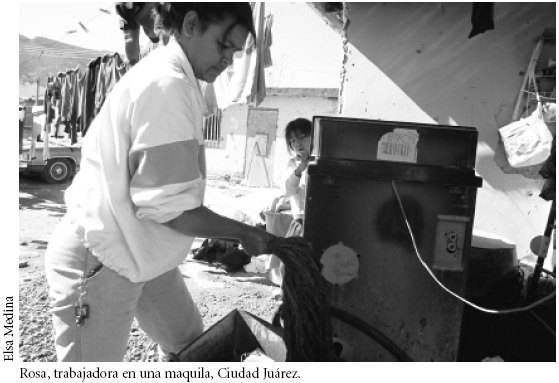
\includegraphics{Img/Rosa.jpg}

}

\caption{Rosa}

\end{figure}%

\subsection{Crecimiento Descontrolado y Desafíos
Urbanos}\label{crecimiento-descontrolado-y-desafuxedos-urbanos}

Ya en los setentas, la maquila era la que rifaba en Juárez. Empleaba a
un chorro de gente, sobre todo a las morras, que eran las que más jale
encontraban en las fábricas de textiles y electrónica {[}6{]}. Pero como
todo en la vida, no todo era miel sobre hojuelas. El crecimiento fue tan
rápido que la ciudad no estaba preparada para tanta gente. Juárez creció
como mancha de aceite, con colonias que brotaban por todos lados, muchas
sin agua, drenaje ni pavimento {[}7{]}.

Las maquilas se instalaban donde les daba la gana, y eso hizo que el
crecimiento urbano fuera un desmadre {[}1{]}. La falta de planificación
hizo que muchas colonias se quedaran sin servicios básicos, y la ciudad,
en lugar de crecer con orden, lo hizo a lo loco. Aun así, la maquila
seguía siendo la que mandaba, y la raza, a pesar de las broncas, no
dejaba de jalar porque, como dicen por aquí, la chamba es la chamba.

\subsection{Crisis y Resiliencia}\label{crisis-y-resiliencia}

Pero no todo fue éxito. En 1974, Juárez se enfrentó a su primera gran
crisis en la maquila cuando la empresa Transformer de México cerró,
dejando a 300 trabajadores en la calle {[}8{]}. La recesión en Estados
Unidos pegó duro, y varias maquilas que dependían del mercado gringo se
vieron en la necesidad de bajar cortinas {[}8{]}. La crisis se volvió a
sentir en 1980, cuando varias fábricas tuvieron que reducir operaciones
o cerrar temporalmente por falta de materia prima y sobreproducción
{[}9{]}.

A pesar de estos golpes, la maquila en Juárez demostró que estaba hecha
de otra madera. En 1983, ya andaba operando al 85\% de su capacidad, y
para 1984, se esperaba que la cosa mejorara aún más con la llegada de
nuevas empresas {[}10{]}{[}11{]}. Fue durante los ochentas cuando Juárez
empezó a atraer a empresas de alta tecnología, marcando una nueva etapa
en la historia de la maquila en la ciudad {[}11{]}. La resiliencia de
Juárez frente a las crisis mostró que, aunque las cosas se pusieran
difíciles, la ciudad siempre encontraba la manera de salir adelante.

\subsection{Evolución Reciente y Desafíos
Modernos}\label{evoluciuxf3n-reciente-y-desafuxedos-modernos}

En los últimos años, la industria maquiladora en Ciudad Juárez ha
seguido siendo un motor económico crucial. Sin embargo, ha tenido que
adaptarse a nuevos desafíos, como la digitalización, la automatización y
los cambios en las cadenas de suministro globales. El impacto de la
pandemia de COVID-19 también obligó a las maquilas a reinventar sus
procesos para mantener la producción en marcha, implementando nuevas
tecnologías y protocolos de seguridad {[}12{]}.

El informe de la Secretaría de Economía de 2022 destaca cómo la
industria maquiladora ha empezado a integrar tecnologías como la
inteligencia artificial y el Internet de las Cosas (IoT) para optimizar
la producción y reducir costos {[}13{]}. Esto ha llevado a una
transformación en la forma en que operan las maquilas, con un enfoque
cada vez mayor en la innovación y la sostenibilidad.

\begin{figure}[H]

{\centering 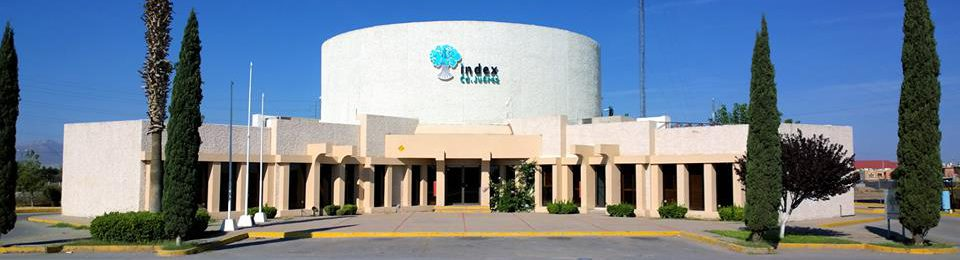
\includegraphics{Img/Amac.jpg}

}

\caption{Amac}

\end{figure}%

\begin{center}\rule{0.5\linewidth}{0.5pt}\end{center}

\subsection{Referencias}\label{referencias}

\begin{enumerate}
\def\labelenumi{\arabic{enumi}.}
\tightlist
\item
  Oscar Martínez, \emph{Ciudad Juárez: El auge de una ciudad fronteriza
  a partir de 1848}, FCE, México, 1982.
\item
  ``La Frontera norte, diagnóstico y perspectivas'', Dirección General
  de Estadística, S.I.C. s/f, mimeo.
\item
  Thomas Madison, \emph{Reseña anual de la industria maquiladora},
  SUGUMEX, México, 1990.
\item
  Bass Zavala, Sonia. ``El crecimiento urbano en Ciudad Juárez,
  1950-2000. Un acercamiento socio-histórico a la evolución desordenada
  de una ciudad de la frontera norte.'' \emph{Chihuahua Hoy} (2013):
  247-289.
\item
  ``La Frontera norte, diagnóstico y perspectivas'', Dirección General
  de Estadística, S.I.C. s/f, mimeo.
\item
  Diario de Juárez, 21 a 24 de agosto de 1981.
\item
  El Fronterizo, 25 de agosto de 1974.
\item
  Guadalupe Ramos, Norte, 9 de febrero de 1994, p.~4A.
\item
  Diario de Juárez, 22 de mayo de 1991.
\item
  Diario de Juárez, 7 de febrero de 1991.
\item
  Declaración de José Manuel Luna, promotor de AMACH, \emph{Novedades},
  20 de enero de 1985.
\item
  Vega, Luis. ``La transformación de la industria maquiladora en la era
  digital.'' \emph{El Financiero}, 2023.
\item
  Secretaría de Economía. ``Informe Anual sobre la Industria
  Maquiladora''. Gobierno de México, 2022.
\end{enumerate}

\bookmarksetup{startatroot}

\chapter{Fundamentos}\label{fundamentos}

\section{Concepto}\label{concepto}

La Inteligencia Artificial (IA) es un término que ha sido parte de la
conversación tecnológica desde hace décadas. Aunque a veces parece un
concepto moderno, sus raíces vienen de los años 50, cuando pioneros como
\textbf{John McCarthy} y \textbf{Herbert A. Simon} empezaron a hablar
sobre la idea de hacer que las máquinas ``piensen'' de manera similar a
los humanos. Según McCarthy, la IA se trata de ``la ciencia e ingeniería
de hacer que las máquinas se comporten de manera inteligente.'' Pero,
¿qué significa esto en términos más simples?

En su libro clásico \textbf{``Las Ciencias de lo Artificial''} (1969),
Simon describió la IA como la habilidad de una máquina para imitar el
pensamiento humano en la toma de decisiones y la resolución de
problemas. Estas ideas nos ayudan a entender que la IA no es magia, sino
una tecnología diseñada para analizar datos, aprender de ellos, y actuar
en consecuencia, a menudo siguiendo reglas o patrones.

\section{Ramas de Inteligencia Artificial
(IA)}\label{ramas-de-inteligencia-artificial-ia}

\begin{figure}[H]

{\centering 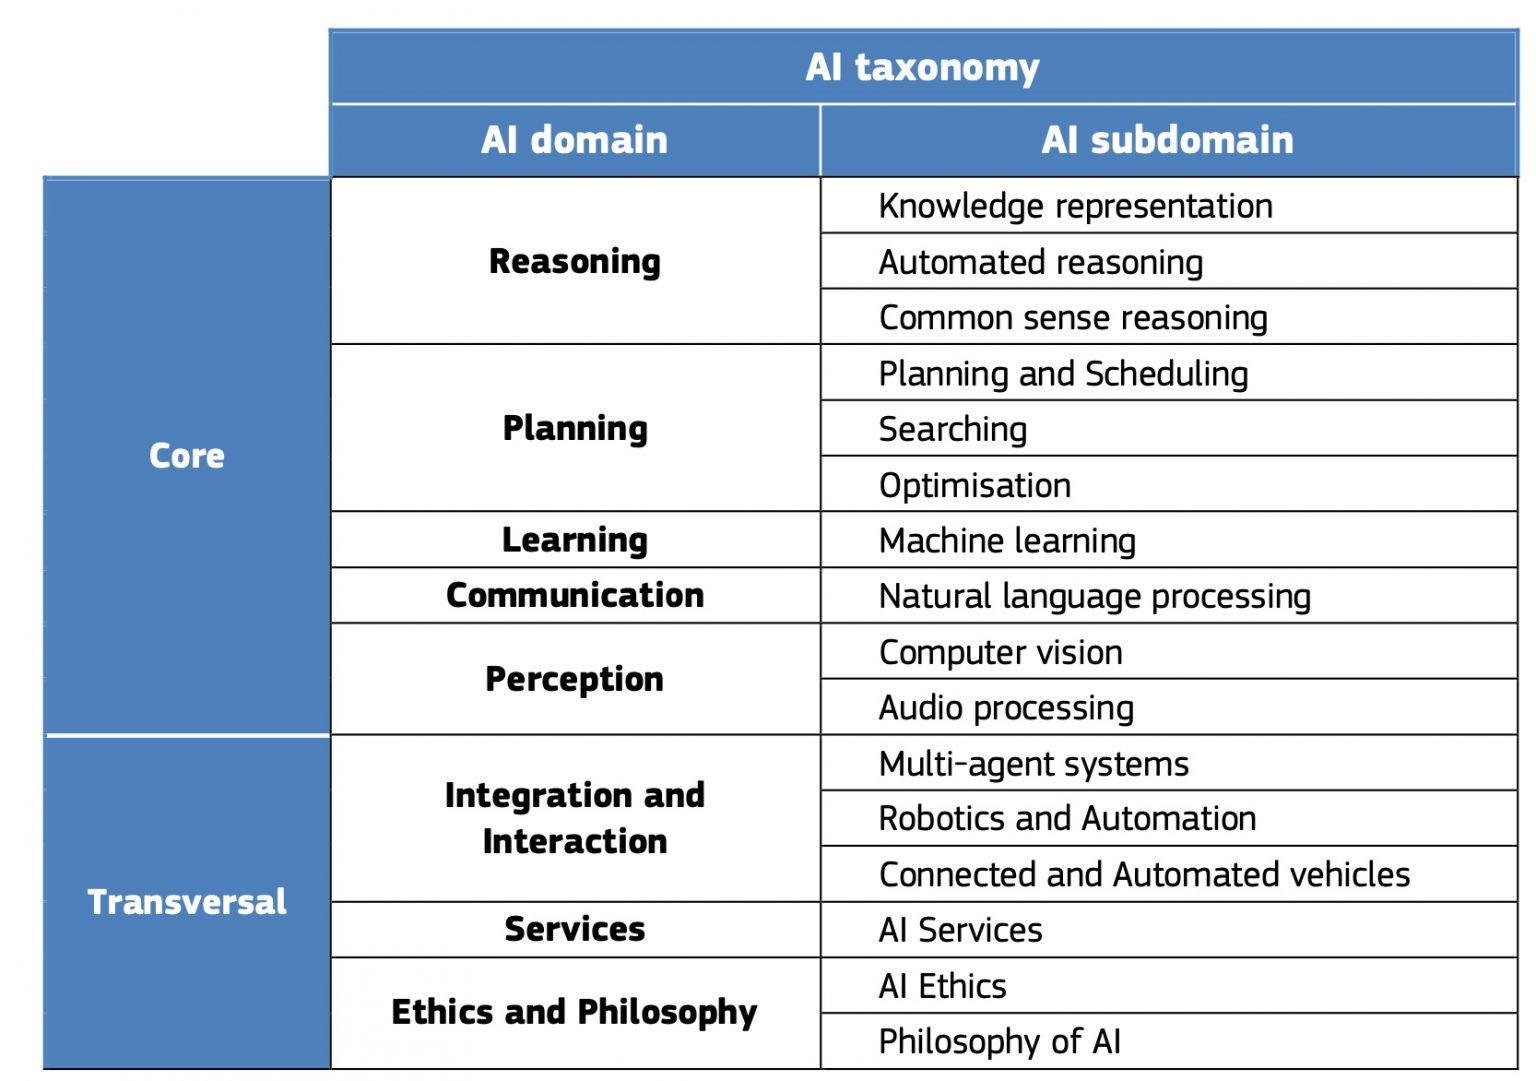
\includegraphics{Img/taxonomia.jpg}

}

\caption{Ramas}

\end{figure}%

Esta imagen presenta una \textbf{taxonomía de la Inteligencia Artificial
(IA)}, organizada en dominios y subdominios, que abarca tanto aspectos
\textbf{centrales (Core)} como \textbf{transversales (Transversal)} de
la IA. Aquí te explico cada sección:

\subsection{Dominio Central (Core):}\label{dominio-central-core}

Estos son los fundamentos o los componentes clave de la IA, que abarcan
desde cómo razona una máquina hasta cómo percibe e interactúa con el
mundo.

\begin{enumerate}
\def\labelenumi{\arabic{enumi}.}
\tightlist
\item
  \textbf{Reasoning (Razonamiento)}:

  \begin{itemize}
  \tightlist
  \item
    \textbf{Knowledge Representation}: Representación del conocimiento.
    Se refiere a cómo una máquina organiza y almacena la información de
    manera que pueda usarla para tomar decisiones o resolver problemas.
  \item
    \textbf{Automated Reasoning}: Razonamiento automatizado. La
    capacidad de la IA para derivar conclusiones y resolver problemas
    complejos basados en las reglas y el conocimiento almacenado.
  \item
    \textbf{Common Sense Reasoning}: Razonamiento de sentido común. La
    IA intenta razonar como lo haría una persona, utilizando
    conocimientos que los humanos damos por sentado, pero que las
    máquinas deben aprender o codificar.
  \end{itemize}
\item
  \textbf{Planning (Planificación)}:

  \begin{itemize}
  \tightlist
  \item
    \textbf{Planning and Scheduling}: Planificación y programación. La
    capacidad de la IA para organizar tareas o recursos en función de
    objetivos, optimizando tiempos y recursos.
  \item
    \textbf{Searching}: Búsqueda. IA encuentra soluciones a problemas o
    información relevante entre un conjunto de opciones.
  \item
    \textbf{Optimisation}: Optimización. Aquí la IA busca la mejor
    solución entre múltiples alternativas, ajustando variables para
    obtener el mejor rendimiento o eficiencia.
  \end{itemize}
\item
  \textbf{Learning (Aprendizaje)}:

  \begin{itemize}
  \tightlist
  \item
    \textbf{Machine Learning}: Aprendizaje automático. Esta es la
    capacidad de las máquinas para aprender a partir de datos sin ser
    programadas explícitamente para cada tarea. Es una de las áreas más
    destacadas y utilizadas en la IA actual.
  \end{itemize}
\item
  \textbf{Communication (Comunicación)}:

  \begin{itemize}
  \tightlist
  \item
    \textbf{Natural Language Processing}: Procesamiento del lenguaje
    natural. La IA comprende, interpreta y genera lenguaje humano,
    facilitando la interacción entre humanos y máquinas mediante el
    habla o el texto.
  \end{itemize}
\item
  \textbf{Perception (Percepción)}:

  \begin{itemize}
  \tightlist
  \item
    \textbf{Computer Vision}: Visión por computadora. La IA percibe el
    mundo visualmente, analizando imágenes o videos para detectar
    patrones, objetos o reconocer caras.
  \item
    \textbf{Audio Processing}: Procesamiento de audio. Similar a la
    visión por computadora, pero en este caso, la IA procesa y entiende
    sonidos, como la voz o música.
  \end{itemize}
\end{enumerate}

\subsection{Dominio Transversal:}\label{dominio-transversal}

Estas áreas complementan los dominios centrales, ofreciendo integración,
interacción y aspectos filosóficos o éticos.

\begin{enumerate}
\def\labelenumi{\arabic{enumi}.}
\tightlist
\item
  \textbf{Integration and Interaction (Integración e Interacción)}:

  \begin{itemize}
  \tightlist
  \item
    \textbf{Multi-agent Systems}: Sistemas multiagente. Conjunto de IA
    que trabajan juntas, colaborando o compitiendo para resolver
    problemas más complejos.
  \item
    \textbf{Robotics and Automation}: Robótica y automatización. Integra
    la IA con robots y sistemas automatizados para realizar tareas
    físicas, como ensamblar productos en fábricas.
  \item
    \textbf{Connected and Automated Vehicles}: Vehículos conectados y
    automatizados. Implica el uso de IA para controlar vehículos
    autónomos y conectados que operan sin intervención humana.
  \end{itemize}
\item
  \textbf{Services (Servicios)}:

  \begin{itemize}
  \tightlist
  \item
    \textbf{AI Services}: Servicios de IA. Herramientas y plataformas
    basadas en IA que las empresas y personas pueden utilizar para
    resolver problemas o mejorar procesos (por ejemplo, asistentes
    virtuales, análisis predictivos).
  \end{itemize}
\item
  \textbf{Ethics and Philosophy (Ética y Filosofía)}:

  \begin{itemize}
  \tightlist
  \item
    \textbf{AI Ethics}: Ética de la IA. Se ocupa de las cuestiones
    éticas relacionadas con el uso y el desarrollo de la IA, como la
    privacidad, la equidad y el impacto social.
  \item
    \textbf{Philosophy of AI}: Filosofía de la IA. Reflexiones más
    profundas sobre el papel de la IA en la sociedad y qué significa
    para las máquinas tener inteligencia similar a la humana.
  \end{itemize}
\end{enumerate}

\begin{center}\rule{0.5\linewidth}{0.5pt}\end{center}

\subsection{Resumen:}\label{resumen}

La taxonomía de la IA presentada en esta imagen divide los conceptos
fundamentales en dominios que abarcan \textbf{razonamiento},
\textbf{planificación}, \textbf{aprendizaje}, \textbf{comunicación} y
\textbf{percepción}. Estos conceptos son claves para entender cómo la IA
interactúa y aprende del mundo. Los dominios transversales complementan
estas capacidades con aspectos como la \textbf{integración}, los
\textbf{servicios de IA} y las \textbf{cuestiones éticas}, que son
fundamentales para asegurar un uso responsable y eficaz de la
inteligencia artificial en el mundo real.

\section{IA Simbólica}\label{ia-simbuxf3lica}

La Inteligencia Artificial Simbólica es un enfoque de la IA que se basa
en representar el conocimiento y el razonamiento a través de símbolos y
reglas lógicas. En lugar de aprender a partir de datos como ocurre en el
Machine Learning, la IA simbólica funciona siguiendo un conjunto de
instrucciones predefinidas para resolver problemas o tomar decisiones.
En este sistema, los programadores crean reglas claras que la máquina
debe seguir, y la IA utiliza estas reglas para tomar decisiones basadas
en relaciones lógicas de ``si-entonces'' o ``condiciones''.

Este enfoque es como una receta: todo está previamente determinado, y la
máquina sigue los pasos sin desviarse. Por ejemplo, un sistema de IA
simbólica podría estar programado para diagnosticar fallos en una
máquina si ciertas condiciones, como la temperatura o la vibración,
exceden los límites establecidos. Cada condición está claramente
definida, y la IA actúa según las reglas sin necesidad de adaptarse o
aprender nuevas formas de solucionar el problema.

La IA simbólica es particularmente útil en entornos donde los procesos
son repetitivos o bien estructurados. En la maquiladora, se usa en casos
como el control de calidad basado en reglas predefinidas o la gestión de
tiempos de producción. Aunque no es flexible como el Machine Learning,
la IA simbólica es extremadamente precisa y eficiente cuando se trata de
ejecutar tareas que siguen un patrón fijo y bien entendido.

La IA Simbólica se utiliza en situaciones donde las reglas y
procedimientos están claramente definidos y son consistentes. Este
enfoque es ideal para procesos repetitivos o controlados, donde se
pueden establecer reglas lógicas y secuencias de pasos que la máquina
debe seguir sin necesidad de aprender o adaptarse. En estos casos, la IA
simbólica es altamente confiable porque sigue estrictamente las
instrucciones que se le proporcionan. Por ejemplo, en una maquiladora,
el ensamblaje de piezas con pasos fijos o la programación de tiempos de
producción puede ser gestionado eficientemente por IA simbólica, ya que
las condiciones no varían mucho y las decisiones se toman en base a
reglas claras.

Además, la IA simbólica se usa en aplicaciones como sistemas expertos,
donde se requiere tomar decisiones basadas en conocimientos específicos,
como el diagnóstico de fallos de máquinas. Aquí, se definen reglas de
``si-entonces'' que guían la toma de decisiones: ``Si la temperatura del
motor sube más de 80°C, entonces apaga la máquina''. Aunque este enfoque
no es flexible ni aprende de los datos, es muy eficaz cuando los
parámetros y resultados son predecibles, y se necesita precisión sin
variaciones.

La IA simbólica se adapta mejor a contextos donde el entorno es estable,
los datos no cambian de manera dinámica, y las decisiones se pueden
programar de antemano. Por eso, en áreas de la maquila como control de
procesos, administración de turnos o mantenimiento bajo condiciones
estándar, sigue siendo una opción confiable y eficiente.

Este tipo de robot es un ejemplo de \textbf{IA Simbólica}, porque sigue
un conjunto de reglas claras para completar la tarea. Cada paso está
definido de manera precisa, y el robot simplemente sigue las
instrucciones. Si la receta no cambia, el robot siempre hará el pastel
de la misma manera, una y otra vez. No necesita aprender ni adaptarse
porque todo está programado de antemano.

En la industria maquiladora, este tipo de IA puede ser útil para tareas
repetitivas como ensamblar piezas, donde las reglas del proceso son
claras y no cambian con el tiempo. \textbf{Imagina} una línea de
producción donde una máquina ensambla componentes electrónicos: coloca
una pieza aquí, ajusta un tornillo allá. Siempre que las instrucciones
sean las mismas, la IA simbólica funciona perfectamente.

\subsubsection{Ejemplo 1: La Receta de Cocina (IA
Simbólica)}\label{ejemplo-1-la-receta-de-cocina-ia-simbuxf3lica}

\textbf{Imagina} que le das a un robot una receta detallada para hacer
un pastel. Le das instrucciones específicas como: 1. Mezcla 200 gramos
de harina con 100 gramos de azúcar. 2. Añade dos huevos y bate la mezcla
por 5 minutos. 3. Coloca la mezcla en el horno a 180°C durante 30
minutos.

\subsubsection{Ejemplo 2: El Chef Aprendiz (Machine
Learning)}\label{ejemplo-2-el-chef-aprendiz-machine-learning}

Ahora, \textbf{imagina} que en lugar de seguir siempre la misma receta,
tienes un robot que quiere convertirse en un chef experto. En lugar de
seguir instrucciones precisas, este robot observa a diferentes cocineros
haciendo pasteles y aprende de sus técnicas. Tal vez nota que algunos
cocineros usan más azúcar, otros agregan ingredientes extra como
vainilla, y algunos hornean el pastel por más tiempo dependiendo del
tipo de horno. El robot comienza a \textbf{aprender} que, dependiendo de
ciertos factores, puede ajustar la receta para hacer el mejor pastel
posible.

Este es un ejemplo de \textbf{Machine Learning}, donde la IA no sigue
reglas predefinidas, sino que aprende a partir de los datos que
recopila. En lugar de seguir la misma receta siempre, el robot adapta la
receta según los datos que ha recopilado (temperatura ambiente, tipo de
ingredientes, preferencias de sabor, etc.).

En una maquiladora, un sistema de \textbf{Machine Learning} puede hacer
lo mismo con tus datos de producción. \textbf{Imagina} que tienes una
máquina que fabrica piezas de plástico, y las condiciones varían según
la temperatura o el tipo de material que estás utilizando. Un sistema de
Machine Learning puede observar estos factores y ajustar automáticamente
los parámetros de la máquina para obtener el mejor rendimiento. Si nota
que la calidad del producto disminuye cuando la temperatura sube más de
cierto punto, aprenderá a ajustar la temperatura para mantener la
calidad.

\subsubsection{Comparando los Enfoques}\label{comparando-los-enfoques}

\begin{itemize}
\item
  \textbf{IA Simbólica}: Es como el robot que sigue una receta fija.
  Funciona bien en situaciones donde las reglas son claras y no cambian
  mucho. Esto es útil en procesos repetitivos como el ensamblaje en una
  maquila, donde los pasos son los mismos cada día.
\item
  \textbf{Machine Learning}: Es como el chef aprendiz. En lugar de
  seguir reglas fijas, aprende y mejora con el tiempo a medida que
  recopila más información. En la maquila, esto es útil en situaciones
  donde hay variabilidad, como ajustes en las máquinas para mejorar la
  calidad o la predicción de fallos en los equipos.
\end{itemize}

\subsubsection{Otro Ejemplo en la Maquiladora: Control de
Calidad}\label{otro-ejemplo-en-la-maquiladora-control-de-calidad}

\textbf{Imagina} que en tu maquila produces miles de piezas cada día, y
necesitas asegurarte de que todas cumplan con los estándares de calidad.
En lugar de tener a una persona revisando cada pieza (lo cual puede ser
lento y propenso a errores), podrías usar \textbf{IA Simbólica} o
\textbf{Machine Learning}.

\begin{itemize}
\item
  Con \textbf{IA Simbólica}, podrías programar una máquina para revisar
  cada pieza siguiendo reglas específicas. Por ejemplo: ``Si la pieza
  tiene más de 0.5 mm de desviación, recházala''. Esto es eficiente,
  pero solo funciona para detectar errores simples.
\item
  Con \textbf{Machine Learning}, podrías entrenar a una máquina para
  detectar patrones más complejos. El sistema podría aprender a
  reconocer qué tipo de defectos aparecen con mayor frecuencia y, con el
  tiempo, predecir dónde y cuándo es más probable que aparezcan
  defectos, ajustando la producción en consecuencia. Podría incluso
  aprender de nuevos datos para mejorar la precisión a lo largo del
  tiempo.
\end{itemize}

\subsubsection{Reflexión Final: Bajar la IA a lo
Práctico}\label{reflexiuxf3n-final-bajar-la-ia-a-lo-pruxe1ctico}

La IA, en su forma más simple, es una herramienta que ayuda a las
máquinas a hacer tareas que normalmente haría un humano, pero con mayor
precisión y eficiencia. No necesitas ser un experto para empezar a
entender cómo puede mejorar tu maquila. Lo importante es reconocer que
hay dos formas principales en que la IA puede ayudarte:
\textbf{siguiendo reglas fijas (IA Simbólica)} o \textbf{aprendiendo de
los datos (Machine Learning)}. Y aunque los conceptos técnicos puedan
sonar complicados, los beneficios prácticos son claros: más eficiencia,
menos errores, y una producción más ágil y adaptada a las necesidades
del día a día.

Al final del día, implementar IA en la maquila puede ser tan sencillo
como hacer un pastel siguiendo una receta, o tan avanzado como un chef
que mejora sus técnicas con cada plato que cocina. Lo importante es
saber cuál enfoque se adapta mejor a tus necesidades y empezar a
aprovecharlo para llevar tu operación al siguiente nivel. ¡A darle!s

\subsection{IA Simbólica: Conceptos Claros con Diagramas de
Flujo}\label{ia-simbuxf3lica-conceptos-claros-con-diagramas-de-flujo}

La Inteligencia Artificial Simbólica es un enfoque donde la IA opera
basándose en reglas predefinidas, es decir, un conjunto de condiciones
lógicas establecidas por programadores que guían las acciones de la
máquina. A continuación, te explico cómo se pueden usar elementos clave
como los diagramas de flujo para implementar IA simbólica de manera
clara y estructurada en un entorno práctico, como una maquiladora.

\textbf{Concepto de IA Simbólica}

La IA simbólica se fundamenta en reglas lógicas que siguen el esquema de
``si-entonces'' (if-then). Esto significa que la máquina ejecutará una
acción dependiendo de si una condición específica se cumple o no.

Por ejemplo:

\begin{itemize}
\tightlist
\item
  Condición: Si la temperatura de la máquina supera los 80°C, entonces
  envía una alerta.
\item
  Condición 2: Si el nivel de stock de un producto es menor a 100
  unidades, entonces genera una orden de compra.
\end{itemize}

Este tipo de razonamiento es ideal para tareas automatizadas y procesos
repetitivos donde las condiciones son predecibles.

\textbf{Elementos Clave para Implementar IA Simbólica}

\begin{itemize}
\tightlist
\item
  \textbf{Diagrama de Flujo}
\end{itemize}

Un diagrama de flujo es una representación gráfica de un proceso. En el
caso de la IA simbólica, se puede utilizar para ilustrar cómo las reglas
lógicas guían el comportamiento del sistema.

\emph{Ejemplo de un diagrama de flujo para IA simbólica:}

\begin{itemize}
\tightlist
\item
  Inicio: El sistema comienza a monitorear la temperatura de la máquina.
\item
  Condición 1: ¿La temperatura es mayor a 80°C?

  \begin{itemize}
  \tightlist
  \item
    Sí: Detener la máquina y enviar alerta al supervisor (acción A).
  \item
    No: Continuar monitoreando (acción B).
  \end{itemize}
\item
  Condición 2: ¿El nivel de stock es menor a 100 unidades?

  \begin{itemize}
  \tightlist
  \item
    Sí: Generar orden de compra automáticamente (acción C).
  \item
    No: Seguir con el proceso de producción (acción D).
  \end{itemize}
\end{itemize}

En este flujo, cada decisión está basada en una condición clara que
lleva a una acción específica. Esto es exactamente cómo funciona la IA
simbólica, ya que sigue reglas de este tipo sin necesidad de aprender o
ajustarse con el tiempo.

\textbf{Ejemplo Aplicado: Sistema de Control de Inventario}

\begin{itemize}
\item
  Escenario: Imagina que en tu maquila tienes un sistema de control de
  inventario. Este sistema necesita generar automáticamente una orden de
  compra cuando el nivel de stock de cierto material cae por debajo de
  un umbral.
\item
  Condiciones Predefinidas:

  \begin{itemize}
  \tightlist
  \item
    Regla 1: Si el stock es menor a 50 unidades, entonces enviar alerta.
  \item
    Regla 2: Si el stock es menor a 10 unidades, generar automáticamente
    una orden de compra.
  \end{itemize}
\item
  Diagrama de Flujo para la IA Simbólica del Inventario:

  \begin{itemize}
  \tightlist
  \item
    Inicio: El sistema verifica el nivel de stock.
  \item
    Condición 1: ¿El stock es menor a 50?

    \begin{itemize}
    \tightlist
    \item
      Sí: Envía alerta al responsable de inventarios.
    \item
      No: Continuar monitoreando.
    \end{itemize}
  \item
    Condición 2: ¿El stock es menor a 10?

    \begin{itemize}
    \tightlist
    \item
      Sí: Generar orden de compra automáticamente.
    \item
      No: Mantener el inventario.
    \end{itemize}
  \end{itemize}
\end{itemize}

\textbf{Referencia:}

\begin{itemize}
\tightlist
\item
  \textbf{Russell, S. J., \& Norvig, P. (2020). \emph{Artificial
  Intelligence: A Modern Approach (4th ed.)}. Pearson.} Este libro es
  una referencia clásica en el campo de la Inteligencia Artificial y
  proporciona una base sólida para comprender los diferentes enfoques,
  incluyendo la IA simbólica. ¡Entiendo lo que estás buscando! Vamos a
  darle un enfoque más \textbf{didáctico} y estructurado, usando listas
  y secciones que faciliten la lectura y el entendimiento, mientras
  mantenemos el mismo contenido. Aquí te dejo la nueva versión:
\end{itemize}

\begin{center}\rule{0.5\linewidth}{0.5pt}\end{center}

\subsection{Capítulo: Las Ventajas de la IA Simbólica: El Primer Paso
Hacia la
Automatización}\label{capuxedtulo-las-ventajas-de-la-ia-simbuxf3lica-el-primer-paso-hacia-la-automatizaciuxf3n}

En cualquier organización, como una maquiladora, el conocimiento
operativo a menudo está centralizado en una persona o en archivos que
pocos pueden entender. Esto puede ser un riesgo significativo, ya que la
dependencia de personas específicas o de sistemas manuales, como
archivos de Excel, puede frenar la eficiencia de los procesos. La
\textbf{IA Simbólica} ofrece una solución práctica para automatizar y
descentralizar este conocimiento, permitiendo que los procesos se
formalicen y ejecuten de manera coherente sin depender de un solo
individuo.

La IA Simbólica funciona mediante reglas predefinidas que permiten a las
máquinas tomar decisiones basadas en condiciones claras, como el clásico
``si-entonces'' (if-then). A continuación, exploramos las ventajas de la
IA Simbólica y por qué representa el primer paso esencial hacia la
automatización inteligente en una maquiladora.

\begin{center}\rule{0.5\linewidth}{0.5pt}\end{center}

\subsubsection{¿Por qué Usar IA Simbólica en Tu
Maquiladora?}\label{por-quuxe9-usar-ia-simbuxf3lica-en-tu-maquiladora}

\begin{enumerate}
\def\labelenumi{\arabic{enumi}.}
\item
  \textbf{Automatización de Tareas Repetitivas}\\
  La IA Simbólica es ideal para procesos donde las condiciones no
  cambian mucho y las reglas pueden definirse claramente. Esto incluye
  tareas como:

  \begin{itemize}
  \tightlist
  \item
    \textbf{Gestión de Inventarios}: Automatizar las órdenes de compra
    cuando los niveles de stock caen por debajo de un umbral.
  \item
    \textbf{Mantenimiento Preventivo}: Detener máquinas o enviar alertas
    cuando ciertos parámetros, como la temperatura, superan los límites
    seguros.
  \end{itemize}
\item
  \textbf{Descentralización del Conocimiento}\\
  Muchas veces, los procesos clave de la empresa dependen de una sola
  persona o de archivos mal organizados. Con la IA Simbólica, la lógica
  del negocio se transfiere a reglas claras y automatizadas, evitando
  que el conocimiento esté centralizado en una sola fuente. Esto reduce
  riesgos y asegura la continuidad del negocio, incluso si el personal
  cambia.
\item
  \textbf{Claridad y Transparencia con Diagramas de Flujo}\\
  Un gran beneficio de la IA Simbólica es la \textbf{visualización de
  procesos} mediante \textbf{diagramas de flujo}. Estos diagramas
  permiten a todos entender cómo se toman las decisiones dentro del
  sistema, lo que facilita la comunicación y mejora la colaboración
  entre departamentos. Un diagrama de flujo podría verse algo así:

  \begin{itemize}
  \tightlist
  \item
    \textbf{Inicio}: El sistema comienza a monitorear la temperatura de
    la máquina.
  \item
    \textbf{Condición 1}: ¿La temperatura es mayor a 80°C?

    \begin{itemize}
    \tightlist
    \item
      \textbf{Sí}: Detener la máquina y enviar una alerta al supervisor.
    \item
      \textbf{No}: Continuar monitoreando.
    \end{itemize}
  \item
    \textbf{Condición 2}: ¿El nivel de stock es menor a 100 unidades?

    \begin{itemize}
    \tightlist
    \item
      \textbf{Sí}: Generar una orden de compra automáticamente.
    \item
      \textbf{No}: Continuar el proceso de producción.
    \end{itemize}
  \end{itemize}

  \textbf{Conclusión:} Este enfoque permite que todos los miembros del
  equipo, desde los operadores hasta los supervisores, entiendan
  claramente cómo se toman las decisiones en cada etapa del proceso.
\end{enumerate}

\begin{center}\rule{0.5\linewidth}{0.5pt}\end{center}

\subsubsection{Ejemplo Práctico: Sistema de Control de
Inventario}\label{ejemplo-pruxe1ctico-sistema-de-control-de-inventario}

\textbf{Escenario:}\\
Imagina que en tu maquiladora manejas grandes cantidades de inventario y
necesitas automatizar el proceso de reabastecimiento. Tradicionalmente,
un encargado del almacén revisa manualmente los niveles de stock y crea
órdenes de compra cuando se está quedando sin material. Este proceso
manual puede ser ineficiente, propenso a errores y muy dependiente de
una sola persona.

\textbf{Con IA Simbólica, este proceso puede automatizarse fácilmente
mediante las siguientes reglas:}

\begin{itemize}
\tightlist
\item
  \textbf{Condición 1}: Si el stock es menor a 50 unidades, enviar una
  alerta.
\item
  \textbf{Condición 2}: Si el stock es menor a 10 unidades, generar
  automáticamente una orden de compra.
\end{itemize}

\textbf{Ventajas para el Negocio:}

\begin{itemize}
\tightlist
\item
  \textbf{Reducción de errores humanos}: No dependerás de que alguien se
  acuerde de revisar los niveles de stock, ya que el sistema lo hará por
  ti.
\item
  \textbf{Eficiencia mejorada}: Al automatizar las órdenes de compra, se
  eliminan retrasos que podrían detener la producción.
\item
  \textbf{Descentralización del proceso}: No importa si el encargado de
  inventarios está presente o no, el sistema seguirá funcionando
  automáticamente.
\end{itemize}

\begin{center}\rule{0.5\linewidth}{0.5pt}\end{center}

\subsubsection{Un mito Famoso en la Comunidad de
Desarrolladores}\label{un-mito-famoso-en-la-comunidad-de-desarrolladores}

Aquí es donde entra un meme que muchos desarrolladores de software
comparten en tono de broma: el meme del programador que, después de
realizar una tarea manual y repetitiva mil veces, finalmente decide
crear un programa para automatizar esa tarea.

\begin{figure}[H]

{\centering 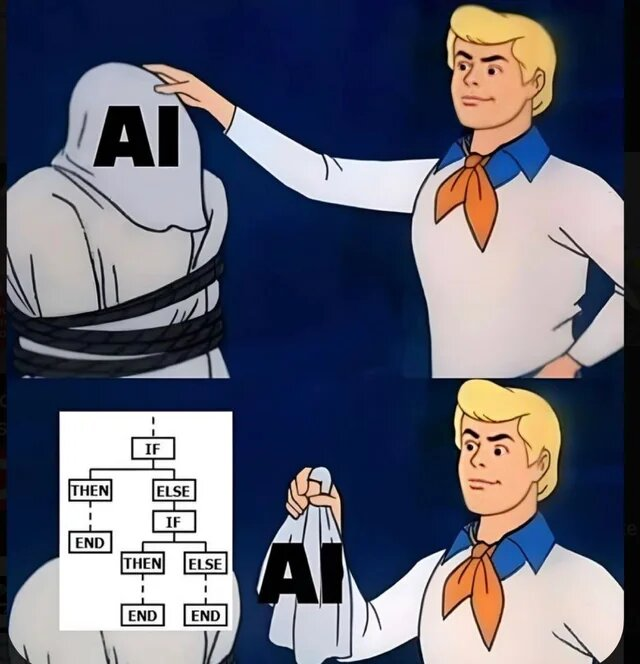
\includegraphics{Img/ia.jpg}

}

\caption{Meme}

\end{figure}%

La IA Simbólica es, en esencia, esa ``solución'' para las tareas
repetitivas en la maquiladora. En lugar de depender de que alguien haga
las mismas tareas una y otra vez, se implementan reglas claras que
permiten que las máquinas lo hagan de forma automática. \textbf{Imagina
la diferencia en eficiencia cuando ya no dependes de una persona que
tenga que hacer manualmente cada ajuste o revisión.}

\begin{center}\rule{0.5\linewidth}{0.5pt}\end{center}

\subsubsection{Ventajas Principales de la IA Simbólica para Tu
Maquiladora}\label{ventajas-principales-de-la-ia-simbuxf3lica-para-tu-maquiladora}

Vamos a resumir las principales ventajas en una lista clara:

\begin{enumerate}
\def\labelenumi{\arabic{enumi}.}
\tightlist
\item
  \textbf{Automatización de procesos repetitivos}: Perfecto para tareas
  donde las reglas no cambian con frecuencia.
\item
  \textbf{Descentralización del conocimiento}: Evita que el conocimiento
  esté retenido por una sola persona o en un archivo difícil de manejar.
\item
  \textbf{Eficiencia y precisión}: Reduce los errores humanos y asegura
  que las tareas se realicen de manera uniforme.
\item
  \textbf{Escalabilidad}: Es fácil modificar las reglas si el proceso o
  las condiciones cambian, haciendo la solución flexible y adaptable.
\item
  \textbf{Mejor colaboración}: Los diagramas de flujo y las reglas son
  fácilmente comprensibles para todos en la organización, facilitando la
  integración entre equipos.
\end{enumerate}

\begin{center}\rule{0.5\linewidth}{0.5pt}\end{center}

\subsubsection{¿Por Qué Empezar con la IA
Simbólica?}\label{por-quuxe9-empezar-con-la-ia-simbuxf3lica}

Si tu maquila aún no ha dado el salto hacia la automatización, la IA
Simbólica es la mejor opción para comenzar. \textbf{Es simple de
implementar, fácil de entender y muy efectiva} para automatizar procesos
que sigan reglas claras. A medida que tu negocio crezca, puedes seguir
construyendo sobre esta base, añadiendo más complejidad y flexibilidad,
pero el primer paso es crucial para reducir la dependencia de sistemas
manuales y asegurar que el conocimiento esté disponible para todos.

\begin{center}\rule{0.5\linewidth}{0.5pt}\end{center}

\subsubsection{Conclusión: El Primer Paso Hacia la Automatización
Inteligente}\label{conclusiuxf3n-el-primer-paso-hacia-la-automatizaciuxf3n-inteligente}

La \textbf{IA Simbólica} es un paso esencial para que tu maquila avance
hacia la automatización y la descentralización del conocimiento. Al
establecer reglas claras y estructuradas, respaldadas por diagramas de
flujo, puedes asegurar que todos los procesos se realicen de manera
eficiente, sin depender de una sola persona o archivo.

Si aún operas en un entorno donde la lógica de negocio está en manos de
unos pocos o donde los procesos manuales dominan, la IA Simbólica es tu
punto de partida ideal. \textbf{Es el primer paso hacia un futuro más
ágil, eficiente y colaborativo.}

\subsection{Perfil para Trabajar con IA Simbólica en una
Maquiladora}\label{perfil-para-trabajar-con-ia-simbuxf3lica-en-una-maquiladora}

Para implementar y gestionar la \textbf{IA Simbólica} en una
maquiladora, se necesita un perfil multidisciplinario que combine
habilidades técnicas con un profundo conocimiento de los procesos
industriales. A continuación, te describo el perfil ideal para alguien
que trabajará en la adopción y gestión de la IA simbólica en un entorno
de producción.

\begin{center}\rule{0.5\linewidth}{0.5pt}\end{center}

\subsection{\texorpdfstring{\textbf{1. Conocimiento Técnico en
Programación y
Lógica}}{1. Conocimiento Técnico en Programación y Lógica}}\label{conocimiento-tuxe9cnico-en-programaciuxf3n-y-luxf3gica}

Dado que la IA simbólica se basa en reglas predefinidas y condiciones
lógicas, es crucial que el candidato tenga sólidos conocimientos de
\textbf{programación} y \textbf{lógica de procesos}. Estos son algunos
de los requisitos técnicos:

\begin{itemize}
\tightlist
\item
  \textbf{Lenguajes de Programación}: Competencia en lenguajes de
  programación que permiten definir reglas y algoritmos, como
  \textbf{Python}, \textbf{C++}, o lenguajes específicos de
  automatización industrial (como \textbf{Ladder Logic} o
  \textbf{Structured Text} para PLCs).
\item
  \textbf{Experiencia en Sistemas de Automatización}: Conocimiento de
  sistemas SCADA o PLC (Controladores Lógicos Programables) que se
  utilizan ampliamente en entornos industriales.
\item
  \textbf{Manejo de Reglas Lógicas}: Habilidad para diseñar y gestionar
  reglas de ``si-entonces'' (if-then) y otros tipos de reglas lógicas
  que determinan el comportamiento de los sistemas de IA simbólica.
\item
  \textbf{Diagramas de Flujo}: Capacidad para diseñar, interpretar y
  modificar diagramas de flujo que describen el funcionamiento del
  sistema de IA simbólica.
\end{itemize}

\subsection{\texorpdfstring{\textbf{2. Conocimiento en Procesos
Industriales}}{2. Conocimiento en Procesos Industriales}}\label{conocimiento-en-procesos-industriales}

Es fundamental que la persona tenga un buen entendimiento de los
procesos específicos de la \textbf{industria maquiladora}. Esto
permitirá al profesional identificar las áreas donde la IA simbólica
puede ser más útil y generar un mayor impacto en la eficiencia y
automatización de procesos.

\begin{itemize}
\tightlist
\item
  \textbf{Control de Calidad}: Comprender cómo funcionan los sistemas de
  control de calidad en la línea de producción y cómo la IA puede
  optimizar el proceso mediante reglas predefinidas para la detección de
  defectos.
\item
  \textbf{Gestión de Inventarios}: Saber cómo operan los sistemas de
  inventario y cómo las reglas lógicas pueden automatizar las órdenes de
  compra y el reabastecimiento.
\item
  \textbf{Mantenimiento de Máquinas}: Conocimiento sobre los ciclos de
  mantenimiento y cómo establecer reglas simbólicas para alertas y
  paradas preventivas.
\end{itemize}

\subsection{\texorpdfstring{\textbf{3. Habilidad para Diseñar Sistemas
Basados en
Reglas}}{3. Habilidad para Diseñar Sistemas Basados en Reglas}}\label{habilidad-para-diseuxf1ar-sistemas-basados-en-reglas}

Una de las tareas más importantes de este perfil es diseñar y optimizar
las reglas que seguirá la IA simbólica. Esto requiere una capacidad para
crear reglas claras y efectivas que cubran todas las posibles
condiciones y escenarios que pueden presentarse en la maquiladora.

\begin{itemize}
\tightlist
\item
  \textbf{Diseño de Reglas Condicionales}: Capacidad para desarrollar un
  sistema de reglas eficiente, asegurándose de que todas las situaciones
  posibles estén cubiertas. Ejemplo: ``Si el nivel de vibración de una
  máquina supera el umbral X, entonces enviar una alerta.''
\item
  \textbf{Optimización de Procesos}: Habilidad para analizar y optimizar
  procesos mediante la creación de flujos lógicos claros, reduciendo
  tiempos muertos y aumentando la eficiencia de la producción.
\end{itemize}

\subsection{\texorpdfstring{\textbf{4. Experiencia en Implementación de
Soluciones de IA
Simbólica}}{4. Experiencia en Implementación de Soluciones de IA Simbólica}}\label{experiencia-en-implementaciuxf3n-de-soluciones-de-ia-simbuxf3lica}

El candidato debe tener experiencia práctica en la implementación de
sistemas basados en IA simbólica, desde el diseño inicial hasta la
puesta en marcha y ajuste de reglas en entornos reales de producción.

\begin{itemize}
\tightlist
\item
  \textbf{Configuración e Integración}: Capacidad para configurar la IA
  simbólica en los sistemas existentes, integrando la tecnología con
  otras soluciones industriales como ERPs, SCADA, o sistemas de gestión
  de inventarios.
\item
  \textbf{Pruebas y Validación}: Habilidad para realizar pruebas y
  validar que las reglas y condiciones están funcionando de acuerdo con
  lo esperado, ajustando según sea necesario para mejorar la precisión
  del sistema.
\end{itemize}

\subsection{\texorpdfstring{\textbf{5. Competencias en Análisis de
Datos}}{5. Competencias en Análisis de Datos}}\label{competencias-en-anuxe1lisis-de-datos}

Aunque la IA simbólica no aprende de los datos como el Machine Learning,
sigue siendo importante que el profesional pueda analizar datos
históricos o de producción para definir reglas de manera efectiva.

\begin{itemize}
\tightlist
\item
  \textbf{Analizar Patrones}: Capacidad para observar patrones en el
  comportamiento de las máquinas, en los tiempos de producción o en los
  niveles de inventario, que puedan traducirse en reglas lógicas.
\item
  \textbf{Generación de Reportes}: Habilidad para generar y analizar
  reportes de producción, eficiencia, y errores detectados por la IA
  simbólica, lo que permitirá afinar las reglas y el sistema.
\end{itemize}

\subsection{\texorpdfstring{\textbf{6. Trabajo en Equipo y
Colaboración}}{6. Trabajo en Equipo y Colaboración}}\label{trabajo-en-equipo-y-colaboraciuxf3n}

La implementación de IA simbólica implica la colaboración con otros
departamentos, como el de producción, mantenimiento, calidad, y TI. El
perfil debe tener buenas \textbf{habilidades de comunicación} y la
capacidad de trabajar en equipo para integrar la tecnología sin causar
fricciones en las operaciones diarias.

\begin{itemize}
\tightlist
\item
  \textbf{Comunicación Interdepartamental}: Capacidad para trabajar con
  ingenieros, operadores de máquinas y personal de TI para diseñar
  reglas que se ajusten a las necesidades de producción.
\item
  \textbf{Capacitación al Personal}: Habilidad para entrenar a los
  operadores y supervisores sobre cómo usar y beneficiarse de los
  sistemas de IA simbólica.
\end{itemize}

\begin{center}\rule{0.5\linewidth}{0.5pt}\end{center}

\subsection{\texorpdfstring{\textbf{Resumen del
Perfil}}{Resumen del Perfil}}\label{resumen-del-perfil}

\begin{enumerate}
\def\labelenumi{\arabic{enumi}.}
\tightlist
\item
  \textbf{Conocimiento Técnico}: Programación, lógica de sistemas, y
  diagramas de flujo.
\item
  \textbf{Entendimiento de Procesos Industriales}: Control de calidad,
  gestión de inventarios y mantenimiento preventivo.
\item
  \textbf{Diseño de Sistemas Basados en Reglas}: Desarrollo de reglas
  condicionales y flujos de decisión claros.
\item
  \textbf{Experiencia Práctica}: Implementación, configuración y ajuste
  de sistemas de IA simbólica en ambientes reales.
\item
  \textbf{Análisis de Datos}: Uso de datos históricos para definir
  reglas efectivas.
\item
  \textbf{Trabajo en Equipo}: Colaboración con distintos departamentos y
  capacidad de entrenamiento al personal.
\end{enumerate}

Este perfil es fundamental para garantizar que la maquiladora pueda
implementar con éxito un sistema de \textbf{IA simbólica} que automatice
tareas repetitivas, mejore la eficiencia y minimice los errores humanos,
todo con un enfoque basado en reglas claras y predefinidas. \#NOTA
AGREAGAR IA NOTA AUTOR

\#\#\# Capítulo: Conocimientos Previos para Machine Learning: Dataset y
Tipos de Variables

El \textbf{Machine Learning (ML)}, o aprendizaje automático, es una rama
de la inteligencia artificial que permite a las máquinas aprender de los
datos y hacer predicciones o tomar decisiones sin ser programadas de
forma explícita para cada tarea. Sin embargo, para comprender cómo
funciona y aprovechar al máximo el Machine Learning en la maquiladora,
primero es necesario entender algunos \textbf{conceptos clave}, como lo
son los \textbf{datasets} y los \textbf{tipos de variables}.

En este capítulo, exploraremos estos conceptos fundamentales que te
permitirán navegar y aplicar con éxito el Machine Learning en tus
procesos industriales.

\begin{center}\rule{0.5\linewidth}{0.5pt}\end{center}

\subsubsection{¿Qué es un Dataset?}\label{quuxe9-es-un-dataset}

Un \textbf{dataset} es simplemente un conjunto de datos que se utiliza
para entrenar y evaluar un modelo de Machine Learning. \textbf{Imagina}
que es como una hoja de cálculo de Excel, donde cada fila es una
instancia o un ejemplo de los datos, y cada columna es una
característica o variable que describe ese ejemplo.

\begin{itemize}
\tightlist
\item
  \textbf{Filas (Instancias)}: Cada fila representa un ejemplo o caso
  dentro del dataset. En el caso de una maquiladora, cada fila podría
  ser un producto individual, una máquina en operación, o una medición
  de calidad.
\item
  \textbf{Columnas (Características/Variables)}: Cada columna describe
  un aspecto o atributo del ejemplo. Esto podría incluir cosas como la
  temperatura de una máquina, el tiempo de operación, o el tamaño de un
  producto.
\end{itemize}

\textbf{Ejemplo en la Maquiladora}: - \textbf{Instancia (Fila)}: Un
producto ensamblado en la línea de producción. - \textbf{Variables
(Columnas)}: Peso del producto, dimensiones, número de piezas
defectuosas, tiempo de ensamblaje, etc.

\subsubsection{Tipos de Datasets}\label{tipos-de-datasets}

En Machine Learning, los datasets se suelen dividir en dos grandes
categorías:

\begin{enumerate}
\def\labelenumi{\arabic{enumi}.}
\item
  \textbf{Dataset de Entrenamiento}: Este es el conjunto de datos que se
  utiliza para entrenar al modelo de Machine Learning. El modelo aprende
  los patrones y relaciones de los datos en este conjunto.
\item
  \textbf{Dataset de Prueba (Test)}: Este conjunto de datos se utiliza
  para evaluar el rendimiento del modelo una vez que ha sido entrenado.
  Es un conjunto nuevo para el modelo, lo que permite medir su capacidad
  de hacer predicciones precisas en datos no vistos antes.
\end{enumerate}

\begin{center}\rule{0.5\linewidth}{0.5pt}\end{center}

\subsubsection{Tipos de Variables}\label{tipos-de-variables}

Al trabajar con Machine Learning, es crucial entender los tipos de
variables que forman parte de tu dataset. Estas variables o
características son las que el modelo va a utilizar para aprender y
hacer predicciones. Existen principalmente dos tipos de variables:
\textbf{variables numéricas} y \textbf{variables categóricas}.

\subsubsection{\texorpdfstring{1. \textbf{Variables
Numéricas}}{1. Variables Numéricas}}\label{variables-numuxe9ricas}

Las \textbf{variables numéricas} son aquellas que representan valores
cuantitativos. Es decir, aquellas que pueden ser medidas en forma de
números y en las que tiene sentido realizar operaciones matemáticas como
suma o promedio. Se dividen en dos tipos:

\begin{itemize}
\item
  \textbf{Variables Continuas}: Pueden tomar un rango infinito de
  valores. \textbf{Ejemplo}: La temperatura de una máquina (35.5°C,
  36.2°C, etc.) o el tiempo de producción de un producto (en horas o
  minutos).
\item
  \textbf{Variables Discretas}: Solo pueden tomar un conjunto limitado
  de valores específicos. \textbf{Ejemplo}: El número de productos
  defectuosos en una línea de producción (1, 2, 3, etc.).
\end{itemize}

\textbf{Ejemplo en la Maquiladora}: - \textbf{Variable Continua}: El
peso de una pieza fabricada. - \textbf{Variable Discreta}: El número de
paradas que tuvo una máquina en un día.

\paragraph{\texorpdfstring{2. \textbf{Variables
Categóricas}}{2. Variables Categóricas}}\label{variables-categuxf3ricas}

Las \textbf{variables categóricas} son aquellas que describen categorías
o grupos. No tienen un valor numérico, sino que clasifican los datos en
diferentes categorías. Se dividen en:

\begin{itemize}
\item
  \textbf{Nominales}: No tienen un orden específico entre las
  categorías. \textbf{Ejemplo}: Los colores de un producto (rojo, azul,
  verde) o los tipos de defectos (fisura, deformación, etc.).
\item
  \textbf{Ordinales}: Tienen un orden jerárquico entre las categorías.
  \textbf{Ejemplo}: La calificación de calidad del producto (alta,
  media, baja) o los niveles de urgencia para el mantenimiento de una
  máquina (alto, medio, bajo).
\end{itemize}

\textbf{Ejemplo en la Maquiladora}: - \textbf{Variable Nominal}: Tipo de
máquina (ensambladora, soldadora, cortadora). - \textbf{Variable
Ordinal}: Clasificación de prioridad para el mantenimiento de máquinas
(urgente, normal, bajo).

\begin{center}\rule{0.5\linewidth}{0.5pt}\end{center}

\subsubsection{¿Por Qué Es Importante Entender los Tipos de
Variables?}\label{por-quuxe9-es-importante-entender-los-tipos-de-variables}

Saber qué tipo de variable estás utilizando en tu dataset es crucial
porque influye en cómo se entrenará el modelo de Machine Learning.
Algunos modelos trabajan mejor con variables numéricas, mientras que
otros pueden manejar variables categóricas.

Por ejemplo: - Un modelo de regresión lineal solo puede trabajar con
\textbf{variables numéricas}. - Un árbol de decisión puede trabajar
tanto con \textbf{variables numéricas} como \textbf{categóricas}.

Además, algunos tipos de variables pueden requerir preprocesamiento
antes de ser usados por un modelo de Machine Learning. \textbf{Las
variables categóricas}, por ejemplo, a menudo deben ser codificadas
(convertidas en números) antes de ser procesadas por el modelo.

\begin{center}\rule{0.5\linewidth}{0.5pt}\end{center}

\subsubsection{Ejemplo en la Maquiladora: Dataset de Mantenimiento
Predictivo}\label{ejemplo-en-la-maquiladora-dataset-de-mantenimiento-predictivo}

Supongamos que deseas implementar un sistema de \textbf{mantenimiento
predictivo} en tu maquiladora, utilizando Machine Learning. Para ello,
necesitas crear un dataset que contenga variables relevantes sobre el
estado de tus máquinas. Este dataset podría verse así:

\begin{longtable}[]{@{}
  >{\raggedright\arraybackslash}p{(\columnwidth - 8\tabcolsep) * \real{0.1412}}
  >{\raggedright\arraybackslash}p{(\columnwidth - 8\tabcolsep) * \real{0.1529}}
  >{\raggedright\arraybackslash}p{(\columnwidth - 8\tabcolsep) * \real{0.2353}}
  >{\raggedright\arraybackslash}p{(\columnwidth - 8\tabcolsep) * \real{0.2000}}
  >{\raggedright\arraybackslash}p{(\columnwidth - 8\tabcolsep) * \real{0.2706}}@{}}
\toprule\noalign{}
\begin{minipage}[b]{\linewidth}\raggedright
ID Máquina
\end{minipage} & \begin{minipage}[b]{\linewidth}\raggedright
Temperatura
\end{minipage} & \begin{minipage}[b]{\linewidth}\raggedright
Horas de Operación
\end{minipage} & \begin{minipage}[b]{\linewidth}\raggedright
Tipo de Máquina
\end{minipage} & \begin{minipage}[b]{\linewidth}\raggedright
Mantenimiento Urgente
\end{minipage} \\
\midrule\noalign{}
\endhead
\bottomrule\noalign{}
\endlastfoot
1 & 85°C & 200 & Soldadora & Sí \\
2 & 70°C & 300 & Ensambladora & No \\
3 & 90°C & 180 & Cortadora & Sí \\
\end{longtable}

\textbf{Variables en el Dataset:} - \textbf{ID Máquina}: Variable
numérica (discreta), utilizada solo para identificar. -
\textbf{Temperatura}: Variable numérica (continua), describe la
temperatura actual de la máquina. - \textbf{Horas de Operación}:
Variable numérica (continua), describe cuántas horas ha estado en
funcionamiento la máquina. - \textbf{Tipo de Máquina}: Variable
categórica (nominal), describe el tipo de máquina. -
\textbf{Mantenimiento Urgente}: Variable categórica (ordinal), indica si
la máquina necesita o no mantenimiento.

Este dataset puede ser usado para entrenar un modelo de Machine Learning
que prediga si una máquina va a necesitar mantenimiento en el futuro. El
modelo analizaría las variables (temperatura, horas de operación, tipo
de máquina) para predecir cuándo será necesario el mantenimiento.

\begin{center}\rule{0.5\linewidth}{0.5pt}\end{center}

\subsubsection{Conclusión}\label{conclusiuxf3n}

Entender los conceptos de \textbf{dataset} y \textbf{tipos de variables}
es fundamental para comenzar a trabajar con \textbf{Machine Learning} en
la maquiladora. Estos conocimientos previos te permitirán preparar tus
datos de manera adecuada, elegir el tipo de modelo más adecuado y lograr
que tu sistema de aprendizaje automático funcione de manera eficiente.

Al manejar correctamente las \textbf{variables numéricas} y
\textbf{categóricas}, y al estructurar bien tu \textbf{dataset}, estarás
dando un paso importante hacia la implementación efectiva de Machine
Learning en tus procesos, ya sea para predecir fallos en las máquinas,
optimizar la calidad del producto o gestionar eficientemente los
inventarios.

Aquí tienes las dos primeras partes del capítulo con más texto y una
explicación menos técnica, adaptada para una mejor comprensión y sin
perder el enfoque en la maquiladora:

\begin{center}\rule{0.5\linewidth}{0.5pt}\end{center}

\section{Aplicaciones de Machine Learning en la
Maquiladora}\label{aplicaciones-de-machine-learning-en-la-maquiladora}

\subsection{\texorpdfstring{\textbf{1. Introducción a Machine Learning
(ML)}}{1. Introducción a Machine Learning (ML)}}\label{introducciuxf3n-a-machine-learning-ml}

El \textbf{Machine Learning} es una herramienta clave en el avance
tecnológico de las maquiladoras. Aunque suena como un concepto
complicado, en realidad es más sencillo de lo que parece: se trata de
enseñar a las máquinas a \textbf{aprender} de los datos, tal como
nosotros aprendemos de la experiencia. En lugar de programar una máquina
para que haga exactamente lo que queremos (como en los sistemas
tradicionales), \textbf{Machine Learning (ML)} permite que las máquinas
identifiquen patrones, hagan predicciones y tomen decisiones basadas en
esos datos.

Entonces, \textbf{¿por qué esto es importante para una maquiladora?}
Porque la IA y el Machine Learning pueden ayudar a reducir errores,
optimizar la producción, mejorar la calidad y anticipar problemas antes
de que ocurran. Si tu línea de producción tiene un historial de fallas
que cuesta tiempo y dinero, ¿no sería genial que una máquina te avisara
antes de que suceda para que pudieras arreglarlo de antemano?

\begin{figure}[H]

{\centering 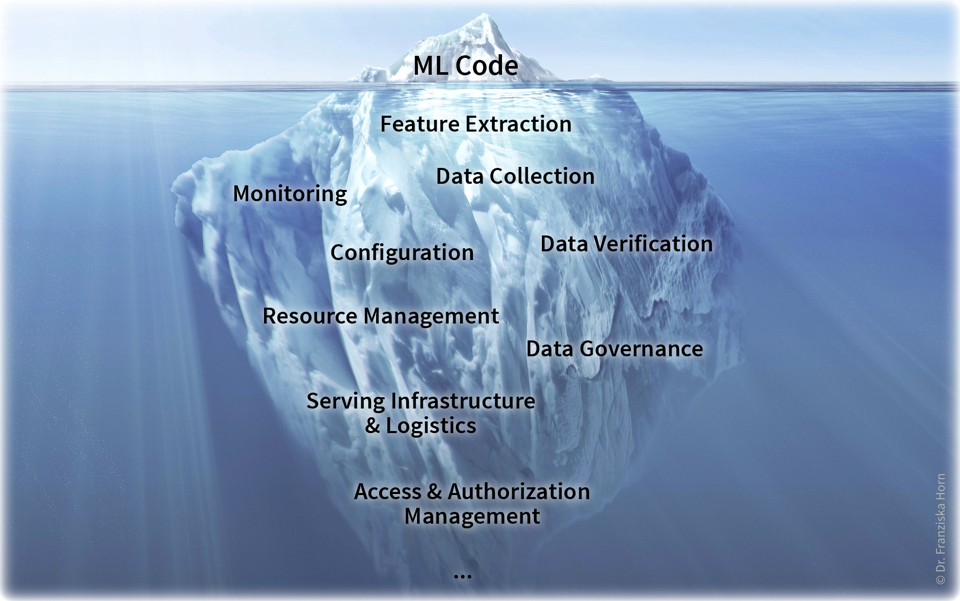
\includegraphics{Img/imagen_186.jpg}

}

\caption{Iceber}

\end{figure}%

\subsubsection{\texorpdfstring{\textbf{1.1. ¿Qué es Machine
Learning?}}{1.1. ¿Qué es Machine Learning?}}\label{quuxe9-es-machine-learning}

El \textbf{Machine Learning} se basa en la idea de que una máquina puede
aprender a hacer algo (como predecir fallas o mejorar un proceso)
simplemente dándole acceso a muchos datos sobre ese algo. \textbf{Es
como enseñar a alguien a resolver un problema dándole ejemplos de cómo
se ha resuelto ese problema antes.}

Imagina que tienes datos sobre la producción de una máquina: las horas
que opera, las temperaturas que alcanza, la cantidad de piezas que
fabrica, etc. Si cada vez que la máquina fallaba también anotabas estas
mismas características, podrías darle esos datos a un modelo de Machine
Learning, y este aprendería a identificar las condiciones que llevan a
una falla. \textbf{Básicamente, se trata de darle a la máquina un
``historial'' de lo que ha pasado, para que pueda predecir lo que pasará
en el futuro}.

En resumen: \textbf{Machine Learning} es el arte de hacer que las
máquinas aprendan de los datos, para que puedan tomar decisiones o hacer
predicciones sin que les digas exactamente qué hacer en cada caso.

\begin{center}\rule{0.5\linewidth}{0.5pt}\end{center}

\subsubsection{\texorpdfstring{\textbf{Supervisado vs No
Supervisado}}{Supervisado vs No Supervisado}}\label{supervisado-vs-no-supervisado}

Existen dos tipos principales de Machine Learning, y entender la
diferencia entre ellos te ayudará a identificar cuál es más útil en tu
maquila.

\subsubsection{\texorpdfstring{\textbf{Aprendizaje
Supervisado}}{Aprendizaje Supervisado}}\label{aprendizaje-supervisado}

El \textbf{aprendizaje supervisado} es como enseñarle a alguien a hacer
algo mostrándole los ejemplos correctos y las respuestas. Le das a la
máquina un conjunto de datos donde ya sabes lo que pasa (el resultado),
y la máquina aprende a predecir ese resultado cuando vea datos nuevos.

\textbf{Ejemplo sencillo en la maquila}: Supón que tienes los datos de
las máquinas en tu línea de producción y sabes qué condiciones llevaron
a una falla (como vibraciones anormales o temperaturas extremas). Puedes
entrenar a un modelo de Machine Learning para que, cuando vea esas
mismas condiciones en una máquina en funcionamiento, te avise de que
algo está mal antes de que ocurra una avería.

Este tipo de ML funciona muy bien cuando ya tienes información sobre lo
que ha ocurrido y quieres predecir lo que sucederá en situaciones
similares en el futuro.

\subsubsection{\texorpdfstring{\textbf{Aprendizaje No
Supervisado}}{Aprendizaje No Supervisado}}\label{aprendizaje-no-supervisado}

Por otro lado, el \textbf{aprendizaje no supervisado} es un poco más
libre: es como darle un montón de información a la máquina y dejarla que
descubra patrones por sí sola. No le dices qué debe buscar, simplemente
la máquina agrupa los datos o encuentra similitudes entre ellos.

\textbf{Ejemplo sencillo en la maquila}: Digamos que tienes muchos datos
sobre el rendimiento de tus máquinas, pero no sabes qué está afectando a
la producción. Con el aprendizaje no supervisado, puedes descubrir
patrones en los datos, como que ciertas máquinas siempre rinden menos a
ciertas horas del día o cuando operan junto a otras máquinas
específicas. La IA encontrará esos patrones, lo que te permitirá hacer
ajustes en la producción que de otro modo no habrías notado.

\begin{center}\rule{0.5\linewidth}{0.5pt}\end{center}

\subsubsection{El papel de ML en la maquila: ¿Por qué es
importante?**}\label{el-papel-de-ml-en-la-maquila-por-quuxe9-es-importante}

Machine Learning puede transformar radicalmente la manera en que operas
en la maquiladora. \textbf{¿Por qué?} Porque la IA no solo se trata de
automatizar, sino de hacer más inteligentes las decisiones que tomas día
a día.

\textbf{Imagina esto}: Tienes una línea de producción donde algunas
máquinas fallan de vez en cuando. Esto significa paradas inesperadas,
retrasos, y por supuesto, costos adicionales. Pero ¿qué pasaría si
pudieras predecir cuándo esas máquinas van a fallar y hacer el
mantenimiento antes de que ocurra la avería? Esto es lo que Machine
Learning puede hacer por ti. Es como tener un ``sexto sentido'' en la
producción.

Además, no solo hablamos de evitar fallas: Machine Learning puede
ayudarte a ajustar el inventario de manera eficiente, prever la demanda,
mejorar la calidad de los productos, y hasta optimizar la logística
dentro de la planta. En resumen, \textbf{es una herramienta para ser más
competitivo en un mercado que no para de moverse}.

\begin{center}\rule{0.5\linewidth}{0.5pt}\end{center}

\subsection{\texorpdfstring{\textbf{Tipos de Machine Learning en la
Maquila}}{Tipos de Machine Learning en la Maquila}}\label{tipos-de-machine-learning-en-la-maquila}

Ahora que ya tienes una idea básica de lo que es Machine Learning y por
qué es tan relevante en la maquiladora, vamos a profundizar un poco más
en los tipos de ML que puedes utilizar en tu planta. Dependiendo del
tipo de problema que enfrentes, puedes elegir entre \textbf{aprendizaje
supervisado} o \textbf{no supervisado}, e incluso otros enfoques como el
\textbf{aprendizaje por refuerzo}.

\begin{figure}[H]

{\centering 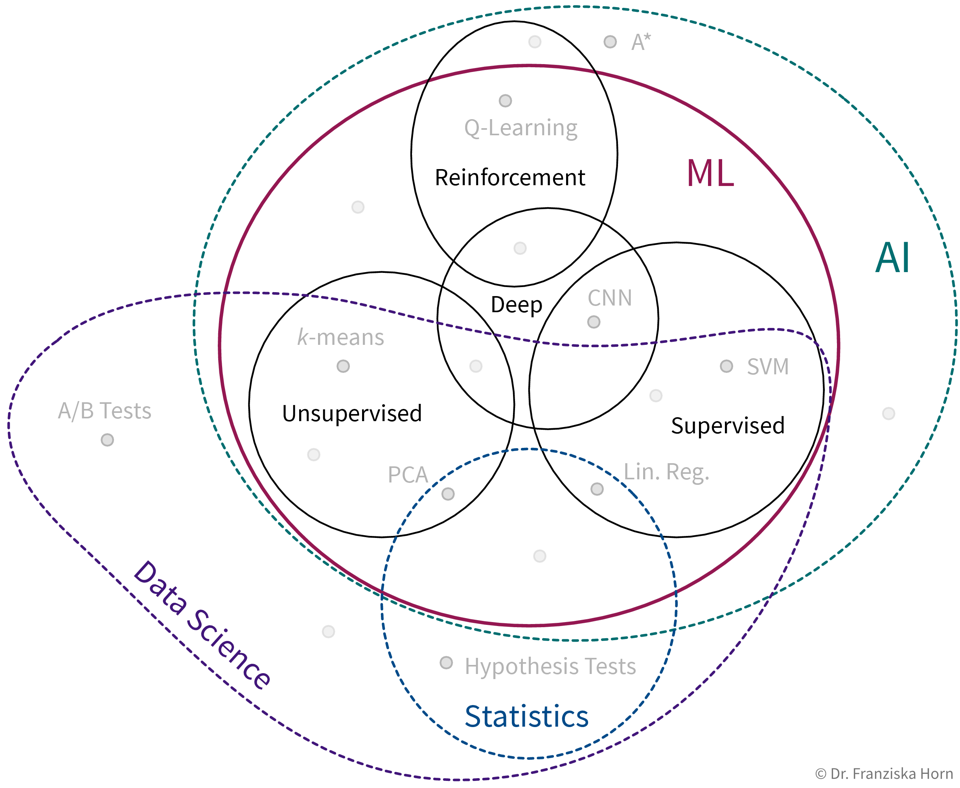
\includegraphics{Img/imagen_21.jpg}

}

\caption{Tipos}

\end{figure}%

\subsubsection{\texorpdfstring{\textbf{Aprendizaje
Supervisado}}{Aprendizaje Supervisado}}\label{aprendizaje-supervisado-1}

En el \textbf{aprendizaje supervisado}, el sistema aprende de datos que
ya incluyen tanto las características (por ejemplo, temperatura de la
máquina, tiempo de operación, etc.) como los resultados correctos (por
ejemplo, si la máquina falló o no). Este tipo de aprendizaje es ideal
cuando ya tienes un montón de información de tus procesos y quieres
usarla para predecir futuros eventos.

\textbf{Ejemplo práctico}: Si sabes que ciertas condiciones en una
máquina han llevado a su falla en el pasado, puedes entrenar un modelo
de aprendizaje supervisado que prediga cuándo una máquina fallará de
nuevo basándose en esas mismas condiciones. Esto es útil para el
\textbf{mantenimiento predictivo}, que puede ahorrarte mucho tiempo y
dinero.

Con aprendizaje supervisado, el sistema va afinando su capacidad de
predecir o clasificar con base en los patrones que ha encontrado en los
datos pasados. Es como si entrenaras a alguien nuevo en tu maquila
mostrándole qué debe hacer y qué no debe hacer con ejemplos concretos.

\subsubsection{\texorpdfstring{\textbf{Aprendizaje No
Supervisado}}{Aprendizaje No Supervisado}}\label{aprendizaje-no-supervisado-1}

El \textbf{aprendizaje no supervisado} es como darle a la máquina una
pila de datos y decirle ``¡descubre algo interesante!''. No le damos las
respuestas de antemano, sino que la máquina encuentra patrones por su
cuenta.

\textbf{Ejemplo práctico}: Puedes usar aprendizaje no supervisado para
analizar datos de producción y descubrir relaciones que no habías visto
antes. Por ejemplo, podrías descubrir que ciertas combinaciones de
máquinas tienden a producir más errores en ciertos momentos del día.
Este tipo de información es oro puro para optimizar la producción, ya
que te permite tomar decisiones informadas basadas en lo que los datos
te dicen, no en suposiciones.

Este enfoque es útil cuando no sabes exactamente qué buscar en tus
datos, pero sospechas que hay información valiosa escondida en ellos. La
máquina encuentra esas conexiones por ti. Gracias por tus comentarios. A
continuación, te dejo el mismo flujo que has aprobado, pero con más
texto para enriquecer los capítulos y dar mayor contexto a cada sección.

\begin{center}\rule{0.5\linewidth}{0.5pt}\end{center}

\subsection{Conceptos Clave para Entender Machine
Learning}\label{conceptos-clave-para-entender-machine-learning}

Para implementar \textbf{Machine Learning (ML)} de manera efectiva en
una maquiladora, es fundamental comprender algunos conceptos clave que
forman la base del aprendizaje automático. Estos términos te ayudarán a
abordar los desafíos técnicos y a tomar decisiones más inteligentes a
medida que avances en tu proceso de transformación digital.

\begin{center}\rule{0.5\linewidth}{0.5pt}\end{center}

\subsubsection{\texorpdfstring{\textbf{Dataset: La Base de
Todo}}{Dataset: La Base de Todo}}\label{dataset-la-base-de-todo}

Un \textbf{dataset} es el conjunto de datos que alimenta al modelo de
Machine Learning. \textbf{Piensa en el dataset como si fuera la materia
prima de una maquiladora}, donde los datos son las piezas que la IA
utiliza para aprender. Sin un buen dataset, el modelo no puede funcionar
correctamente.

\textbf{Ejemplo en la maquila}: Supongamos que tienes datos históricos
sobre las temperaturas de las máquinas, el tiempo que han estado
operativas, el número de piezas que han producido y cuándo fallaron. Ese
conjunto de datos es el ``dataset'' que alimentará tu modelo para que
pueda aprender a predecir cuándo fallará una máquina en el futuro.

Es importante tener en cuenta que la calidad de los datos es
fundamental. Si los datos son incorrectos o incompletos, el modelo
aprenderá mal. Es lo que decimos en Machine Learning: \textbf{``Garbage
in, garbage out''}. Si le das basura al modelo, los resultados también
serán basura.

\begin{center}\rule{0.5\linewidth}{0.5pt}\end{center}

\subsubsection{\texorpdfstring{\textbf{Variables Dependientes e
Independientes}}{Variables Dependientes e Independientes}}\label{variables-dependientes-e-independientes}

En Machine Learning, las \textbf{variables} son los elementos de los
datos que influyen en los resultados. Hay dos tipos de variables que
debes conocer:

\begin{figure}[H]

{\centering 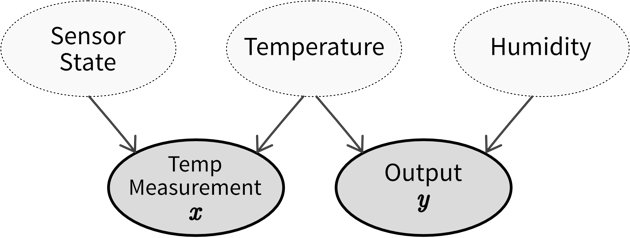
\includegraphics{Img/imagen_157.jpg}

}

\caption{Iceb}

\end{figure}%

\begin{itemize}
\item
  \textbf{Variables Independientes}: Son las entradas que proporcionan
  la información al modelo. Son como las características que describen
  un producto en una maquiladora. Por ejemplo, la temperatura de una
  máquina, la velocidad de producción o el número de horas trabajadas.
\item
  \textbf{Variable Dependiente}: Es la salida o el resultado que estamos
  intentando predecir. Es lo que queremos que la máquina aprenda a
  identificar o calcular. En una maquiladora, la variable dependiente
  podría ser si una máquina va a fallar o no, o la cantidad de piezas
  defectuosas que produce una línea de producción.
\end{itemize}

\textbf{Ejemplo práctico en producción}: Si estás tratando de predecir
fallos en tus máquinas, las variables independientes podrían ser la
vibración de las máquinas, la temperatura y las horas de operación. La
variable dependiente sería si la máquina falla o no.

El éxito de un modelo de Machine Learning depende de cuán bien
seleccionemos estas variables. Un buen conjunto de variables
independientes puede mejorar dramáticamente el rendimiento del modelo.

\begin{center}\rule{0.5\linewidth}{0.5pt}\end{center}

\subsubsection{\texorpdfstring{\textbf{Feature Engineering: La Clave del
Éxito}}{Feature Engineering: La Clave del Éxito}}\label{feature-engineering-la-clave-del-uxe9xito}

El \textbf{feature engineering} es el proceso de elegir, transformar y
crear las características (variables) que mejoran el rendimiento de un
modelo de Machine Learning. Este paso es esencial porque no todas las
variables son igual de útiles. Algunas variables pueden ser
irrelevantes, mientras que otras pueden tener un impacto significativo
en los resultados.

\textbf{Ejemplo en la maquila}: Si estás entrenando un modelo para
predecir cuándo fallará una máquina, probablemente no tenga sentido
incluir la \textbf{marca de la máquina} como una variable independiente.
Sin embargo, la \textbf{temperatura de operación} o la \textbf{cantidad
de horas trabajadas} probablemente sean factores mucho más importantes
que debes incluir.

El \textbf{feature engineering} te ayuda a seleccionar las variables
clave y a descartarlas irrelevantes. También puedes crear nuevas
variables a partir de las existentes. Por ejemplo, si tienes el dato de
la \textbf{temperatura} y el \textbf{número de horas trabajadas},
podrías crear una nueva variable que sea la \textbf{combinación de ambos
factores}, lo que podría mejorar las predicciones.

\begin{center}\rule{0.5\linewidth}{0.5pt}\end{center}

\subsubsection{\texorpdfstring{\textbf{Preprocesamiento de Datos:
Limpiando los
Datos}}{Preprocesamiento de Datos: Limpiando los Datos}}\label{preprocesamiento-de-datos-limpiando-los-datos}

El \textbf{preprocesamiento de datos} es uno de los pasos más
importantes para que un modelo de Machine Learning funcione
correctamente. \textbf{Imagina que tienes un coche muy potente, pero las
llantas están desinfladas. No importa qué tan bueno sea el motor, el
coche no va a funcionar bien.} Lo mismo pasa con los datos: si no están
limpios y organizados, tu modelo no rendirá como debería.

El preprocesamiento implica varias tareas, como: - \textbf{Limpieza de
Datos}: A veces, los datos están incompletos o tienen errores. Por
ejemplo, una máquina podría haber dejado de registrar datos durante
ciertos periodos de tiempo. En este caso, podrías necesitar eliminar
esos datos incompletos o estimar los valores que faltan.

\begin{itemize}
\tightlist
\item
  \textbf{Normalización}: Si tus variables tienen diferentes escalas,
  puede ser útil normalizarlas para que el modelo las procese
  correctamente. Por ejemplo, si una variable mide \textbf{horas de
  operación} (que puede ser un número muy grande) y otra mide
  \textbf{temperatura} (que es un número más pequeño), puedes escalarlas
  para que el modelo las trate de manera equilibrada.
\end{itemize}

El preprocesamiento es clave porque \textbf{los datos crudos no siempre
son útiles}. Limpiarlos y prepararlos adecuadamente te permite sacar el
máximo provecho de tu modelo de Machine Learning.

\begin{figure}[H]

{\centering 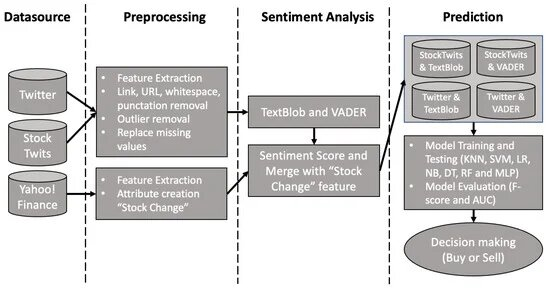
\includegraphics{Img/datasource.jpg}

}

\caption{Dataflow}

\end{figure}%

\begin{center}\rule{0.5\linewidth}{0.5pt}\end{center}

\subsection{Ventajas del Machine Learning en la
Maquiladora}\label{ventajas-del-machine-learning-en-la-maquiladora}

El \textbf{Machine Learning} ofrece muchas ventajas para una
maquiladora, desde la reducción de costos hasta la mejora en la
eficiencia de los procesos. Aquí te detallamos las principales razones
por las que integrar ML en tu maquila puede marcar la diferencia:

\begin{center}\rule{0.5\linewidth}{0.5pt}\end{center}

\subsubsection{\texorpdfstring{\textbf{Rapidez en la Toma de
Decisiones}}{Rapidez en la Toma de Decisiones}}\label{rapidez-en-la-toma-de-decisiones}

Una de las mayores ventajas del Machine Learning es la
\textbf{velocidad} con la que puede analizar grandes cantidades de datos
y ofrecer resultados. Esto es especialmente útil en una maquiladora,
donde la rapidez en la toma de decisiones puede marcar la diferencia
entre cumplir con un pedido o retrasarse.

\textbf{Ejemplo en la maquila}: Un modelo de ML puede analizar los datos
de rendimiento de las máquinas en tiempo real y enviar alertas
instantáneas cuando detecte que algo no está bien. Esto te permite
actuar de inmediato, evitando que pequeños problemas se conviertan en
grandes fallos.

\begin{center}\rule{0.5\linewidth}{0.5pt}\end{center}

\subsubsection{\texorpdfstring{\textbf{Facilidad de Uso y
Sencillez}}{Facilidad de Uso y Sencillez}}\label{facilidad-de-uso-y-sencillez}

Hoy en día, las herramientas de Machine Learning son cada vez más
accesibles, y muchas de ellas ofrecen interfaces simples que no
requieren conocimientos avanzados en programación. Incluso si tu equipo
no tiene experiencia con IA, \textbf{plataformas como AWS, Azure y
Google Cloud} te permiten implementar modelos de manera sencilla y
escalable.

\begin{center}\rule{0.5\linewidth}{0.5pt}\end{center}

\subsubsection{\texorpdfstring{\textbf{Auditoría y
Transparencia}}{Auditoría y Transparencia}}\label{auditoruxeda-y-transparencia}

Otra ventaja clave es que \textbf{los modelos de Machine Learning pueden
ser auditados}. Esto significa que puedes rastrear y verificar cómo el
modelo llegó a una decisión o predicción, lo que es muy importante en
industrias reguladas como la manufactura. Además, te permite ajustar los
modelos con base en los resultados que obtienes.

\textbf{Ejemplo en la maquila}: Si tu modelo predice que una máquina va
a fallar, puedes revisar los datos en los que basó esa predicción (como
la temperatura o la vibración) y ajustar las condiciones si crees que el
modelo está siendo demasiado sensible o no lo suficiente.

\begin{center}\rule{0.5\linewidth}{0.5pt}\end{center}

\subsection{Desventajas del Machine Learning en la
Maquiladora}\label{desventajas-del-machine-learning-en-la-maquiladora}

Aunque \textbf{Machine Learning} tiene muchas ventajas, no es una
solución mágica. Implementarlo también tiene desafíos y posibles
desventajas que debes tener en cuenta.

\begin{center}\rule{0.5\linewidth}{0.5pt}\end{center}

\subsubsection{\texorpdfstring{\textbf{Costo de
Implementación}}{Costo de Implementación}}\label{costo-de-implementaciuxf3n}

A pesar de las ventajas a largo plazo, el costo inicial de implementar
ML puede ser alto, especialmente si tu maquiladora no tiene ya la
infraestructura necesaria. \textbf{La compra de software, hardware
especializado y la contratación de talento} para administrar los
sistemas de Machine Learning pueden representar una barrera.

\textbf{Ejemplo}: Algunas maquiladoras pequeñas podrían no tener acceso
a los recursos necesarios para implementar ML de manera inmediata, por
lo que un enfoque escalonado o la externalización de servicios puede ser
una opción.

\begin{center}\rule{0.5\linewidth}{0.5pt}\end{center}

\subsubsection{\texorpdfstring{\textbf{Dudas
Técnicas}}{Dudas Técnicas}}\label{dudas-tuxe9cnicas}

El éxito de un sistema de Machine Learning depende mucho de la calidad
de los datos y del personal capacitado que pueda supervisar y ajustar
los modelos. Si no tienes un equipo con experiencia en \textbf{análisis
de datos} y \textbf{programación}, podrías enfrentar dificultades para
configurar y mantener el sistema.

\begin{center}\rule{0.5\linewidth}{0.5pt}\end{center}

\subsubsection{\texorpdfstring{\textbf{Complejidad en el Análisis de
Datos}}{Complejidad en el Análisis de Datos}}\label{complejidad-en-el-anuxe1lisis-de-datos}

El análisis de datos en Machine Learning no es una tarea sencilla.
Requiere tiempo y experiencia para preparar correctamente los datos,
seleccionar las variables adecuadas y ajustar los modelos. Además, los
datos en bruto que provienen de las máquinas a menudo tienen errores o
inconsistencias que deben resolverse antes de alimentar al modelo.

\begin{center}\rule{0.5\linewidth}{0.5pt}\end{center}

\subsection{Conclusión de las Ventajas y
Desventajas}\label{conclusiuxf3n-de-las-ventajas-y-desventajas}

En resumen, el \textbf{Machine Learning} tiene el potencial de
revolucionar la maquiladora, optimizando procesos, reduciendo costos y
mejorando la calidad de los productos

. Sin embargo, la implementación tiene desafíos que deben considerarse
cuidadosamente. Con una buena planificación, inversión y el equipo
adecuado, \textbf{ML puede transformar la operación de tu maquila y
mantenerte competitivo en un mercado global}.

\subsection{Referencias ML}\label{referencias-ml}

\begin{enumerate}
\def\labelenumi{\arabic{enumi}.}
\item
  Russell, S. \& Norvig, P. \emph{Artificial Intelligence: A Modern
  Approach} (4th ed.). Prentice Hall, 2020.
\item
  Goodfellow, I., Bengio, Y. \& Courville, A. \emph{Deep Learning}. MIT
  Press, 2016.
\item
  Hastie, T., Tibshirani, R. \& Friedman, J. \emph{The Elements of
  Statistical Learning: Data Mining, Inference, and Prediction} (2nd
  ed.). Springer, 2009.
\item
  Géron, A. \emph{Hands-On Machine Learning with Scikit-Learn, Keras,
  and TensorFlow} (2nd ed.). O'Reilly Media, 2019.
\item
  Murphy, K. P. \emph{Machine Learning: A Probabilistic Perspective}.
  MIT Press, 2012.
\item
  Bishop, C. M. \emph{Pattern Recognition and Machine Learning}.
  Springer, 2006.
\item
  Domingos, P. \emph{The Master Algorithm: How the Quest for the
  Ultimate Learning Machine Will Remake Our World}. Basic Books, 2015.
\item
  Martínez, Oscar. \emph{Ciudad Juárez: El auge de una ciudad fronteriza
  a partir de 1848}. FCE, México, 1982.
\item
  Dirección General de Estadística, S.I.C. \emph{La Frontera Norte,
  Diagnóstico y Perspectivas}. Mimeo.
\item
  Madison, Thomas. \emph{Reseña Anual de la Industria Maquiladora}.
  SUGUMEX, México, 1990.
\item
  Bass Zavala, Sonia. ``El crecimiento urbano en Ciudad Juárez,
  1950-2000. Un acercamiento socio-histórico a la evolución desordenada
  de una ciudad de la frontera norte.'' \emph{Chihuahua Hoy} (2013):
  247-289.
\item
  Diario de Juárez, 21 a 24 de agosto de 1981.
\item
  El Fronterizo, 25 de agosto de 1974.
\item
  Ramos, Guadalupe. \emph{Norte}, 9 de febrero de 1994, p.~4A.
\item
  Diario de Juárez, 22 de mayo de 1991.
\item
  Diario de Juárez, 7 de febrero de 1991.
\item
  Luna, José Manuel. Declaración en \emph{Novedades}, 20 de enero de
  1985.
\item
  Vega, Luis. ``La transformación de la industria maquiladora en la era
  digital.'' \emph{El Financiero}, 2023.
\item
  Secretaría de Economía. ``Informe Anual sobre la Industria
  Maquiladora''. Gobierno de México, 2022.
\end{enumerate}

\bookmarksetup{startatroot}

\chapter{Industria La Industria Maquiladora en Ciudad
Juárez}\label{industria-la-industria-maquiladora-en-ciudad-juuxe1rez}

\section{Evolución de la Industria: La Revolución
Informática}\label{evoluciuxf3n-de-la-industria-la-revoluciuxf3n-informuxe1tica}

La industria maquiladora en Ciudad Juárez no solo ha experimentado una
evolución en sus procesos productivos, sino que también ha sido parte de
una revolución informática que ha transformado profundamente la manera
en que se gestiona y opera. Este cambio fue un proceso gradual que
comenzó con herramientas básicas como los procesadores de hojas de
cálculo, avanzó hacia los sistemas de planificación de recursos
empresariales (ERP) y continúa evolucionando con las tecnologías
modernas.

\subsubsection{Procesadores de Hojas de Cálculo: Los Primeros
Pasos}\label{procesadores-de-hojas-de-cuxe1lculo-los-primeros-pasos}

Antes de que los sistemas ERP llegaran a las maquilas, las primeras
herramientas informáticas que cambiaron la manera de trabajar en las
oficinas fueron los procesadores de hojas de cálculo. En los años 80,
programas como Lotus 1-2-3 y más tarde Microsoft Excel, se convirtieron
en herramientas esenciales para la gestión de datos. Estas hojas de
cálculo permitieron a los gerentes y administradores realizar cálculos
complejos, llevar un registro de inventarios y analizar datos con mayor
precisión que nunca antes.

Los procesadores de hojas de cálculo fueron una auténtica revolución
porque permitieron que las operaciones diarias de las maquilas se
volvieran más organizadas y eficientes. Antes de estas herramientas,
muchos cálculos se hacían a mano o con calculadoras, lo que era un
proceso lento y propenso a errores. Con la llegada de las hojas de
cálculo, los datos se podían manipular, analizar y presentar de manera
mucho más rápida y precisa, lo que mejoró la toma de decisiones y la
eficiencia operativa en las plantas.

Aunque las hojas de cálculo siguen siendo una herramienta valiosa hoy en
día, especialmente para tareas más sencillas, su uso exclusivo se ha
vuelto insuficiente para manejar las complejidades de las operaciones
modernas en la industria maquiladora. A medida que las empresas
crecieron y sus operaciones se volvieron más complejas, surgió la
necesidad de sistemas más integrados y robustos, dando paso a la llegada
de los ERPs.

\begin{figure}[H]

{\centering 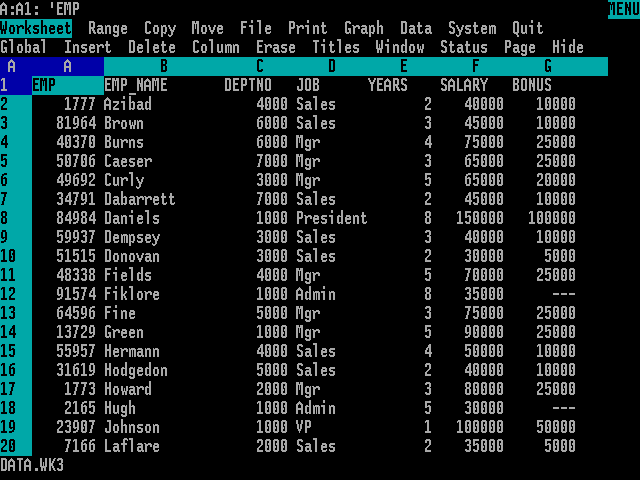
\includegraphics{Img/Lotus.png}

}

\caption{Hoja de cálculo}

\end{figure}%

\subsubsection{Primeros ERPs: La Llegada de AS400 de
IBM}\label{primeros-erps-la-llegada-de-as400-de-ibm}

La revolución informática en la maquila realmente despegó con la llegada
de sistemas como el AS400 de IBM. Este sistema, que se volvió un
verdadero pilar en la gestión de operaciones, fue una herramienta que
cambió las reglas del juego. Antes del AS400, muchas de las tareas
administrativas se hacían de manera manual o con hojas de cálculo, con
mucho esfuerzo y un alto margen de error. Con la implementación del
AS400, las empresas pudieron llevar un control más preciso de sus
inventarios, producción y distribución. Este sistema permitió a las
maquilas en Juárez mejorar la eficiencia operativa, reducir costos y
tomar decisiones más informadas.

\begin{figure}[H]

{\centering 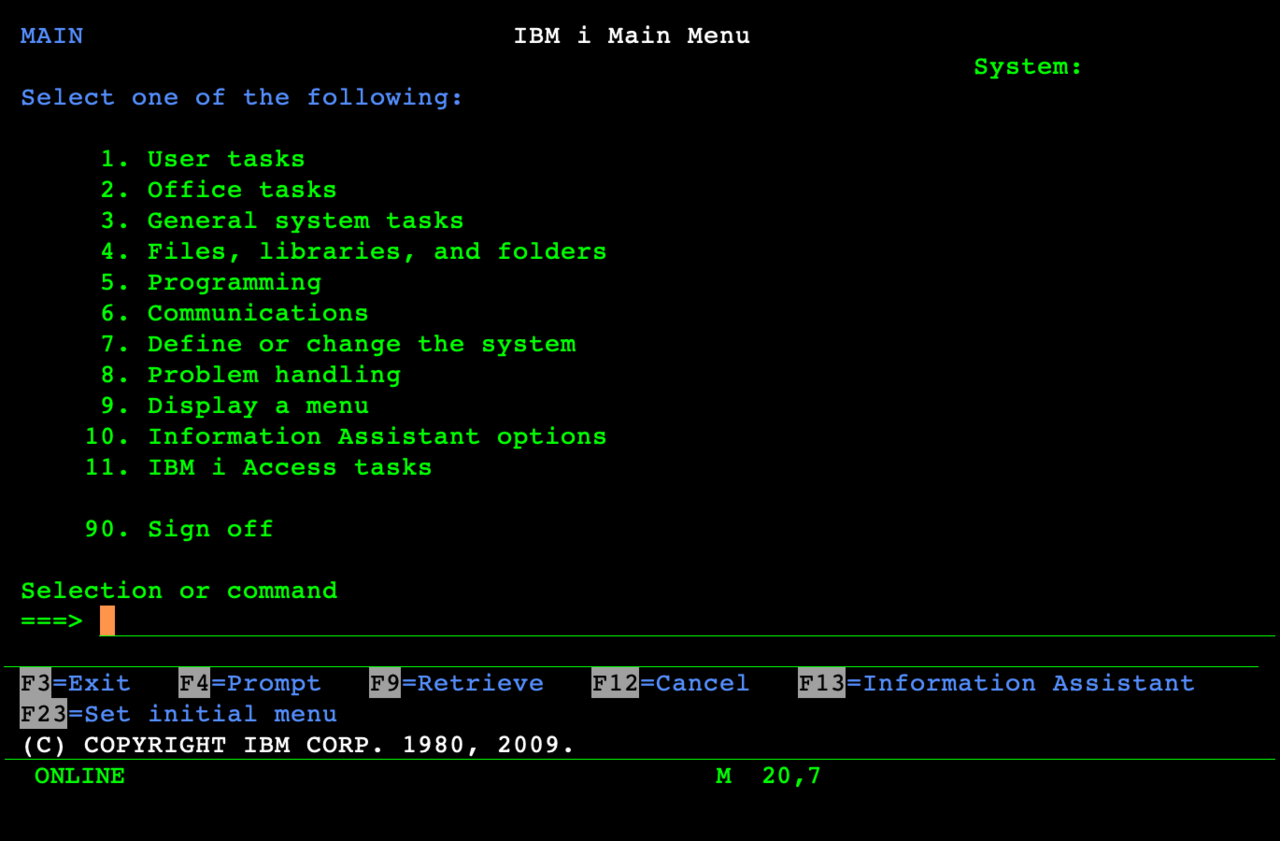
\includegraphics{Img/ibm.png}

}

\caption{IBM}

\end{figure}%

Sin embargo, el AS400, que fue tan revolucionario en su momento, ha
quedado desfasado con el tiempo. Hoy en día, sigue siendo utilizado en
algunas empresas, pero la realidad es que es un sistema que ya no se
actualiza y que está limitado en comparación con las tecnologías
actuales. Si todavía estás usando un AS400 en tu maquila, es hora de que
empieces a pensar en una actualización, porque aferrarse a tecnologías
descontinuadas puede poner en riesgo la competitividad y la agilidad de
tu empresa.

\subsubsection{Oracle ERP: Innovación en la Gestión
Empresarial}\label{oracle-erp-innovaciuxf3n-en-la-gestiuxf3n-empresarial}

El siguiente gran salto en la revolución informática vino con Oracle
ERP. Este sistema no solo se enfocó en la gestión de operaciones, sino
que integró finanzas, recursos humanos, y la gestión de la cadena de
suministro en un solo paquete. Oracle ERP permitió a las maquilas en
Juárez operar de manera más eficiente, con una mejor integración entre
sus diferentes áreas. Los gerentes ya no tomaban decisiones basadas en
corazonadas; ahora podían apoyarse en datos precisos y en tiempo real.
Esto mejoró significativamente la toma de decisiones y la capacidad de
respuesta ante problemas.

Pero, al igual que con el AS400, Oracle ERP en sus versiones más
antiguas ha empezado a quedar obsoleto. Aunque Oracle sigue siendo un
líder en soluciones ERP, las versiones más antiguas de su software ya no
reciben soporte completo. Si tu empresa sigue operando con estas
versiones, es hora de considerar una migración a soluciones más modernas
que puedan ofrecerte la flexibilidad y las capacidades que necesitas
para competir en el entorno actual.

\subsubsection{Microsoft CRM: La Era de la Relación con el
Cliente}\label{microsoft-crm-la-era-de-la-relaciuxf3n-con-el-cliente}

La introducción de Microsoft CRM marcó otro hito en la revolución
informática al enfocar las operaciones más allá de lo interno y
dirigirse hacia la gestión de relaciones con los clientes. En un mercado
tan competitivo como el de la maquila, donde la lealtad del cliente es
clave, contar con un sistema que permita gestionar estas relaciones de
manera eficiente es crucial. Microsoft CRM permitió a las empresas
maquiladoras no solo rastrear sus ventas y marketing, sino también
anticiparse a las necesidades de sus clientes, mejorando la satisfacción
y fidelización.

No obstante, las primeras versiones de Microsoft CRM también han quedado
atrás en el tiempo. Con la llegada de soluciones más avanzadas como
Microsoft Dynamics 365, las empresas tienen ahora herramientas mucho más
potentes y flexibles para gestionar sus relaciones con los clientes. Si
tu maquila sigue utilizando versiones antiguas de CRM, es vital que
consideres actualizarte a versiones más recientes que te permitan
mantener una ventaja competitiva.

\begin{figure}[H]

{\centering 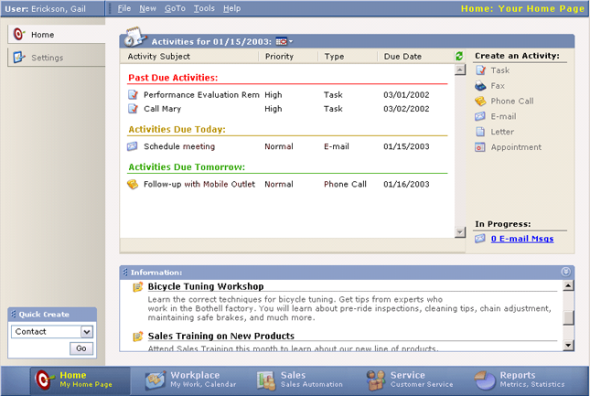
\includegraphics{Img/crm.png}

}

\caption{CRM}

\end{figure}%

\begin{quote}
``Allá por 2015, en mis primeros jales, me tocó trabajar con sistemas de
IBM y Microsoft, y la neta, fue una experiencia bien surrealista. El
software era pirata, y la documentación, ni se diga, hecha en Word por
la misma empresa. Todo un desmadre. Pasaba horas intentando hacer
funcionar esas versiones obsoletas, en proyectos que parecían no tener
fin. Esa experiencia me dejó claro que trabajar con tecnología vieja y
sin soporte es como andar a tientas. Y ¿sabes qué? Esa es la principal
razón por la que muchas empresas medianas siguen usando Excel hoy en
día. El soporte con esos sistemas viejos era tan complicado que la raza
prefería regresarse a lo básico, donde al menos sabían que podían sacar
el trabajo sin tanto pedo. Por eso, estar al tiro con las herramientas
que usas es clave, porque si no, los proyectos se te hacen eternos y
terminas batallando más de la cuenta.''

\textbf{- Javier Flores}
\end{quote}

\subsubsection{La Continuidad de la Revolución
Informática}\label{la-continuidad-de-la-revoluciuxf3n-informuxe1tica}

Estos sistemas, que en su momento fueron revolucionarios, han marcado un
antes y un después en la industria maquiladora de Ciudad Juárez. Sin
embargo, como toda tecnología, han llegado a un punto donde su utilidad
ha disminuido frente a nuevas soluciones más avanzadas. La tecnología no
se detiene, y lo que fue innovador hace 10 o 20 años, hoy puede ser una
carga si no se actualiza. Mantener sistemas descontinuados no solo
limita la capacidad operativa de una empresa, sino que también la expone
a riesgos de seguridad y a una mayor ineficiencia.

Hoy en día, las maquilas en Juárez y en todo el mundo están adoptando
nuevas tecnologías que van más allá de lo que estos primeros ERPs podían
ofrecer. La inteligencia artificial, el análisis de grandes volúmenes de
datos (Big Data), la automatización avanzada y la integración con el
Internet de las Cosas (IoT) están transformando nuevamente la industria.
Por eso, si tu empresa sigue usando sistemas como el AS400, Oracle ERP
en versiones antiguas, o las primeras versiones de Microsoft CRM, es
hora de pensar seriamente en una actualización.

Actualizarte no es solo una opción, es una necesidad si quieres mantener
tu maquila competitiva en un mundo que no deja de evolucionar. La
revolución informática no se detiene, y quienes no se adapten corren el
riesgo de quedarse rezagados en un mercado que cada vez exige más
agilidad, flexibilidad y capacidad de respuesta.

En resumen, la revolución informática ha sido un motor de cambio para la
industria maquiladora, pero la misma revolución exige que no nos
quedemos estancados en el pasado. Si estás utilizando estos sistemas, es
momento de dar el siguiente paso y modernizar tus herramientas para
asegurar que tu empresa siga rifando en la cima de la competitividad
global.

\subsection{Evolución de la Industria: Hacia el Uso de SAP y Otros ERP
Modernos}\label{evoluciuxf3n-de-la-industria-hacia-el-uso-de-sap-y-otros-erp-modernos}

Después de la era del AS400 de IBM, Oracle ERP y Microsoft CRM, la
industria maquiladora en Ciudad Juárez, como en muchas partes del mundo,
comenzó a mirar hacia sistemas más robustos y avanzados que pudieran
manejar la creciente complejidad de las operaciones. Aquí es donde entra
en juego SAP, que se ha convertido en el estándar para la gestión
empresarial en grandes organizaciones. Pero mientras SAP domina en las
grandes ligas, el uso de Excel sigue siendo fuerte en las empresas más
pequeñas, y el desarrollo de ERPs propios también ha ganado terreno,
especialmente entre medianas y pequeñas empresas.

\subsubsection{SAP: El Titán de los
ERP}\label{sap-el-tituxe1n-de-los-erp}

SAP llegó con la promesa de una integración total. Este sistema ofrece
una solución todo-en-uno que abarca desde la gestión de finanzas hasta
la planificación de la producción, la gestión de recursos humanos, la
cadena de suministro, y más. Para las maquilas grandes, SAP se convirtió
en una herramienta esencial para mantener todo bajo control, permitiendo
un nivel de integración y eficiencia que simplemente no era posible con
los sistemas anteriores.

Lo chido de SAP es que permite a las empresas centralizar toda su
información en una base de datos única, lo que facilita la toma de
decisiones en tiempo real. Además, su capacidad para adaptarse a
diferentes industrias y modelos de negocio lo ha convertido en una
opción preferida por muchas de las maquilas más grandes en Juárez. Sin
embargo, la implementación de SAP no es cosa fácil ni barata. Requiere
de una inversión significativa en tiempo, dinero y capacitación, lo que
hace que no todas las empresas puedan acceder a esta tecnología.

SAP también viene con su propio hardware empresarial, y aunque esto
garantiza un rendimiento óptimo, también significa un costo adicional
considerable. Para muchas maquilas, esta inversión vale la pena por el
nivel de control y eficiencia que SAP ofrece. Sin embargo, este mismo
nivel de complejidad y costo hace que SAP no sea una opción viable para
todas las empresas, especialmente para las más pequeñas o aquellas que
prefieren una solución más flexible y menos costosa.

\subsubsection{Excel: La Herramienta de Confianza para las Pequeñas
Empresas}\label{excel-la-herramienta-de-confianza-para-las-pequeuxf1as-empresas}

Mientras que SAP domina en las grandes empresas, Excel sigue siendo el
rey en las empresas más pequeñas y medianas. ¿Por qué? La respuesta es
simple: Excel es barato, casi gratis, y extremadamente flexible. Para
muchas empresas, especialmente las más chicas, Excel es suficiente para
manejar sus necesidades diarias de gestión de datos. Es fácil de usar,
no requiere una gran inversión inicial, y casi todos en la oficina ya
saben cómo usarlo.

Excel permite a estas empresas hacer todo, desde el control de
inventarios hasta la planificación financiera, sin necesidad de sistemas
complejos y caros. Además, el hecho de que no se dependa de un soporte
técnico complicado lo hace aún más atractivo. La raza puede resolver la
mayoría de los problemas por su cuenta, y eso es una ventaja enorme
cuando no tienes un equipo de TI dedicado o cuando el soporte de
sistemas más grandes es demasiado caro o difícil de conseguir.

Es interesante notar cómo, a pesar de la llegada de herramientas mucho
más avanzadas, Excel sigue siendo la opción preferida para muchas
empresas. Su accesibilidad y facilidad de uso lo hacen prácticamente
imbatible en el día a día de las operaciones más pequeñas. Es cierto que
no ofrece la integración y las capacidades de un ERP completo, pero para
muchas empresas, lo ``de a gratis'' y funcional de Excel supera
cualquier desventaja, especialmente cuando los recursos son limitados.

\subsubsection{ERP Propios: Innovación y
Adaptación}\label{erp-propios-innovaciuxf3n-y-adaptaciuxf3n}

Otra tendencia interesante en la industria es el desarrollo de ERPs
propios, especialmente en lenguajes como C\# y Java. Muchas empresas
medianas han optado por crear sus propios sistemas en lugar de adoptar
soluciones como SAP, debido a la flexibilidad que esto ofrece. Al
desarrollar su propio ERP, estas empresas pueden adaptarlo exactamente a
sus necesidades, evitando el pago de licencias caras y el enfrentarse a
sistemas que pueden ser demasiado complejos para sus operaciones.

El desarrollo de estos ERPs propios no es solo una cuestión de ahorro en
licencias, sino también una respuesta a la necesidad de personalización.
Utilizando lenguajes de programación orientada a objetos (POO) como C\#
y Java, los desarrolladores pueden crear sistemas que se ajusten
perfectamente a las operaciones específicas de la empresa. La POO
permite estructurar el código de manera más modular y flexible, lo que
facilita el mantenimiento y la ampliación del software según las
necesidades cambiantes de la empresa.

Además, con la capacidad de crear y gestionar bases de datos a medida,
estas empresas pueden manejar grandes volúmenes de datos de manera
eficiente, sin depender de soluciones preconstruidas que pueden no
adaptarse perfectamente a su modelo de negocio. Los sistemas ERP
desarrollados internamente también permiten a las empresas implementar
procesos de negocio únicos que los sistemas estándar no pueden manejar.

Esta capacidad de personalización y control es especialmente importante
en un entorno tan dinámico como el de la maquila, donde los requisitos
pueden cambiar rápidamente debido a las demandas del mercado o las
regulaciones gubernamentales. Con un ERP propio, las empresas pueden
responder a estos cambios con mayor agilidad, ajustando el software
según sea necesario.

El desarrollo de ERPs propios también está estrechamente relacionado con
la evolución de la ingeniería en sistemas dentro de las empresas. A
medida que más compañías medianas comienzan a ver los beneficios de
tener su propio ERP, la demanda de ingenieros en sistemas capaces de
desarrollar, implementar y mantener estos sistemas ha aumentado. Este
tipo de desarrollo interno no solo reduce la dependencia de proveedores
externos, sino que también fomenta una cultura de innovación dentro de
la empresa, donde los empleados están constantemente buscando nuevas
formas de mejorar y optimizar los procesos.

En resumen, mientras que las grandes maquilas pueden permitirse sistemas
sofisticados como SAP, las pequeñas y medianas empresas encuentran en
Excel y en el desarrollo de sus propios sistemas la solución perfecta
para sus necesidades. El equilibrio entre costo, funcionalidad y
adaptabilidad es crucial para cualquier empresa que busque mantenerse
competitiva en un mercado cada vez más complejo y exigente.

Al final del día, cada empresa debe evaluar su situación y elegir la
herramienta que mejor se adapte a sus necesidades. Sin embargo, lo que
queda claro es que la flexibilidad y la capacidad de adaptación son
clave para el éxito en la competitiva industria maquiladora de Ciudad
Juárez. Y ya sea utilizando Excel, invirtiendo en SAP, o desarrollando
un ERP propio en C\# o Java, lo importante es que las empresas sigan
evolucionando junto con la tecnología, manteniendo sus operaciones
eficientes y preparadas para los desafíos del futuro.

\section{La Llegada de la Industria 4.0: Más Allá del
ERP}\label{la-llegada-de-la-industria-4.0-muxe1s-alluxe1-del-erp}

Con la evolución de la tecnología y la creciente complejidad de las
operaciones en la industria maquiladora, Ciudad Juárez ha sido testigo
de una nueva transformación: la llegada de la Industria 4.0. Este
concepto, que va más allá de la simple automatización, ha introducido un
cambio profundo en la manera en que las maquilas operan, integrando
tecnologías avanzadas no solo en los sistemas ERP, sino también en otras
áreas clave de la producción y la gestión empresarial.

\subsection{Industria 4.0: Una Nueva Era de
Integración}\label{industria-4.0-una-nueva-era-de-integraciuxf3n}

La Industria 4.0, también conocida como la Cuarta Revolución Industrial,
se refiere a la integración de tecnologías avanzadas como el Internet de
las Cosas (IoT), la inteligencia artificial (IA), la robótica avanzada,
y la analítica de datos en tiempo real en los procesos industriales.
Este enfoque permite a las maquilas optimizar sus operaciones, mejorar
la eficiencia, y crear productos de mayor calidad, todo mientras se
reduce el desperdicio y se mejora la sostenibilidad.

Esta revolución no es solo una continuación de las tecnologías
anteriores, sino un cambio de paradigma en cómo se diseñan, operan y
gestionan las plantas de producción. La integración total de sistemas,
desde la planificación hasta la ejecución, permite que cada parte del
proceso esté conectada y se comunique en tiempo real, lo que facilita
una eficiencia operativa sin precedentes y una flexibilidad única para
responder a las necesidades del mercado.

\subsection{Redes y PLC: La Infraestructura de la Industria
4.0}\label{redes-y-plc-la-infraestructura-de-la-industria-4.0}

Además de las tecnologías mencionadas, la base sobre la cual se
construye la Industria 4.0 incluye una infraestructura robusta de redes
y sistemas de control, como los PLCs (Controladores Lógicos
Programables).

\begin{enumerate}
\def\labelenumi{\arabic{enumi}.}
\tightlist
\item
  \textbf{Redes Industriales:}

  \begin{itemize}
  \tightlist
  \item
    Las redes industriales son la columna vertebral de la Industria 4.0.
    Permiten la comunicación entre todos los dispositivos, máquinas y
    sistemas dentro de una planta de producción. Las redes como Ethernet
    Industrial, Profinet y EtherCAT son esenciales para garantizar que
    la información fluya de manera rápida y segura entre los diferentes
    componentes del sistema.
  \item
    Estas redes no solo conectan las máquinas dentro de una planta, sino
    que también permiten la integración con sistemas externos, como los
    de proveedores y clientes. Esto facilita la coordinación a lo largo
    de toda la cadena de suministro, permitiendo una mayor eficiencia y
    una mejor sincronización entre la producción y la demanda.
  \end{itemize}
\end{enumerate}

\begin{figure}[H]

{\centering 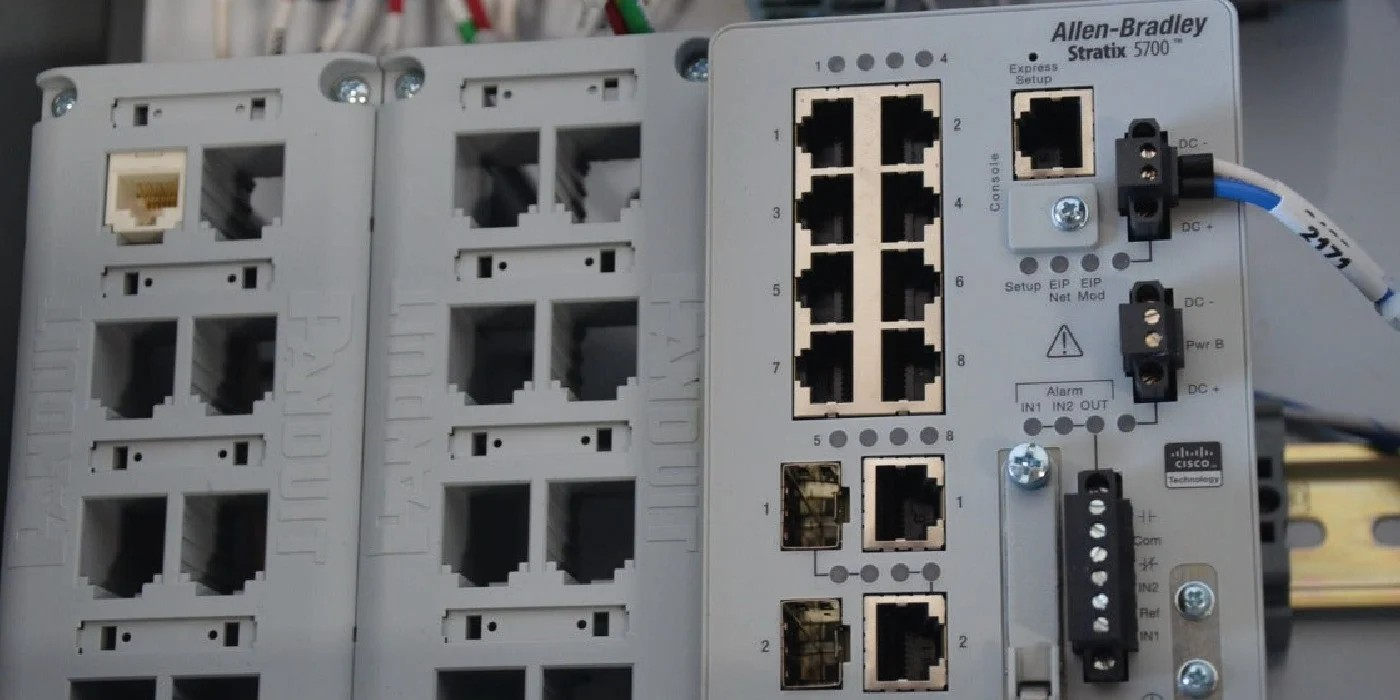
\includegraphics{Img/ethernet.png}

}

\caption{Redes}

\end{figure}%

\begin{enumerate}
\def\labelenumi{\arabic{enumi}.}
\setcounter{enumi}{1}
\tightlist
\item
  \textbf{PLCs y Control de Procesos:}

  \begin{itemize}
  \tightlist
  \item
    Los PLCs han sido una parte integral de la automatización industrial
    durante décadas, y su rol ha evolucionado con la llegada de la
    Industria 4.0. Ahora, los PLCs no solo controlan máquinas
    individuales, sino que también se integran con sistemas más grandes,
    como los ERPs y los sistemas de IoT, para proporcionar un control
    más sofisticado y en tiempo real de los procesos de producción.
  \item
    Los PLCs modernos son capaces de manejar una enorme cantidad de
    datos y realizar cálculos complejos, lo que permite un control más
    preciso y eficiente de los procesos de producción. Además, su
    capacidad de conectarse a redes industriales y compartir datos con
    otros sistemas hace que sean un componente esencial en la
    infraestructura de la Industria 4.0.
  \end{itemize}
\end{enumerate}

\begin{figure}[H]

{\centering 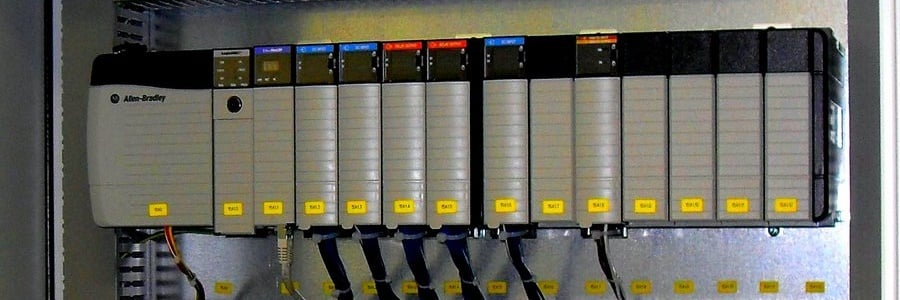
\includegraphics{Img/plc.jpg}

}

\caption{PLC}

\end{figure}%

\begin{enumerate}
\def\labelenumi{\arabic{enumi}.}
\setcounter{enumi}{2}
\tightlist
\item
  \textbf{Sistemas SCADA (Supervisión, Control y Adquisición de Datos):}

  \begin{itemize}
  \tightlist
  \item
    Los sistemas SCADA juegan un papel crucial en la supervisión y
    control de los procesos industriales. En la Industria 4.0, los
    sistemas SCADA se integran con IoT y analítica de datos para
    proporcionar una visión completa y en tiempo real de las
    operaciones, permitiendo a los operadores y gerentes tomar
    decisiones rápidas basadas en datos precisos.
  \item
    Estos sistemas permiten monitorizar en tiempo real las variables
    críticas del proceso, como la temperatura, presión, velocidad de las
    máquinas, etc., y ajustarlas automáticamente para mantener la
    eficiencia y la calidad.
  \end{itemize}
\end{enumerate}

\begin{figure}[H]

{\centering 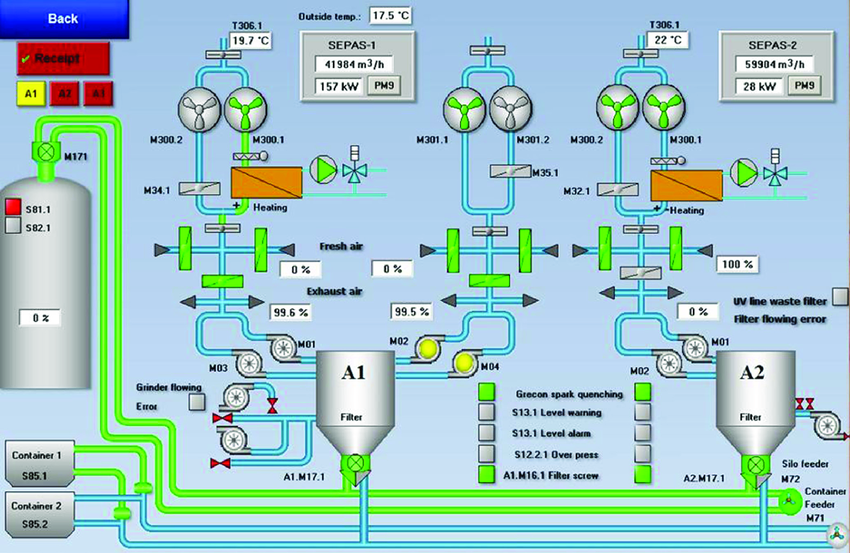
\includegraphics{Img/scada.png}

}

\caption{SCADA}

\end{figure}%

\subsection{La Expansión de los Sistemas
Empresariales}\label{la-expansiuxf3n-de-los-sistemas-empresariales}

La Industria 4.0 también ha impulsado la expansión de los sistemas más
allá de la gestión de recursos empresariales (ERP). Con la creciente
necesidad de integración y eficiencia, las empresas maquiladoras han
comenzado a adoptar una variedad de sistemas especializados que
complementan y amplían las capacidades del ERP tradicional:

\begin{enumerate}
\def\labelenumi{\arabic{enumi}.}
\tightlist
\item
  \textbf{Sistemas de Gestión de la Cadena de Suministro (SCM):}

  \begin{itemize}
  \tightlist
  \item
    Los sistemas SCM se han vuelto críticos en la Industria 4.0, donde
    la sincronización y la coordinación de la cadena de suministro son
    fundamentales. Estos sistemas permiten a las maquilas gestionar de
    manera más eficiente sus relaciones con proveedores, optimizar los
    inventarios y asegurar que los materiales lleguen justo a tiempo
    para la producción.
  \item
    Con la integración de tecnologías IoT y analítica de datos, los
    sistemas SCM pueden proporcionar visibilidad en tiempo real de toda
    la cadena de suministro, permitiendo a las empresas anticiparse a
    problemas antes de que ocurran y ajustar sus operaciones para evitar
    interrupciones.
  \end{itemize}
\item
  \textbf{Sistemas de Gestión de la Relación con el Cliente (CRM):}

  \begin{itemize}
  \tightlist
  \item
    Los sistemas CRM también han evolucionado con la Industria 4.0,
    integrando datos de diferentes fuentes para ofrecer una visión más
    completa del cliente. Esto permite a las maquilas personalizar sus
    productos y servicios de acuerdo con las necesidades del cliente,
    mejorando la satisfacción y fidelización.
  \item
    Con la ayuda de la IA y la analítica avanzada, los sistemas CRM
    pueden predecir las necesidades del cliente antes de que se
    expresen, lo que permite a las empresas adelantarse a la competencia
    y ofrecer soluciones más rápidas y efectivas.
  \end{itemize}
\item
  \textbf{Sistemas de Gestión del Ciclo de Vida del Producto (PLM):}

  \begin{itemize}
  \tightlist
  \item
    Los sistemas PLM gestionan todo el ciclo de vida de un producto,
    desde su diseño inicial hasta su retiro del mercado. En la Industria
    4.0, los PLM se integran con otros sistemas para permitir un
    desarrollo más rápido y eficiente de productos, facilitando la
    colaboración entre departamentos y mejorando la gestión del
    conocimiento.
  \item
    Estos sistemas permiten a las empresas maquiladoras mantener un
    seguimiento de todas las versiones y modificaciones de un producto a
    lo largo de su ciclo de vida, asegurando que la información esté
    siempre actualizada y accesible.
  \end{itemize}
\end{enumerate}

\subsection{Retos y Oportunidades en la Industria
4.0}\label{retos-y-oportunidades-en-la-industria-4.0}

La adopción de la Industria 4.0 trae consigo tanto retos como
oportunidades para las maquilas de Ciudad Juárez. Por un lado, la
inversión en nuevas tecnologías y la reestructuración de los procesos
internos pueden ser costosos y complejos. La necesidad de formación
continua y la integración de múltiples sistemas también pueden
representar desafíos significativos.

Sin embargo, las oportunidades que ofrece la Industria 4.0 son
igualmente grandes. La capacidad de mejorar la eficiencia, reducir
costos, y ofrecer productos personalizados en menos tiempo proporciona
una ventaja competitiva significativa. Además, la integración de
sistemas y la capacidad de tomar decisiones basadas en datos en tiempo
real permiten a las empresas responder más rápidamente a las demandas
del mercado y adaptarse a los cambios de manera más efectiva.

En resumen, la llegada de la Industria 4.0 ha llevado a la industria
maquiladora de Ciudad Juárez a un nuevo nivel de

sofisticación y eficiencia. Las empresas que logren integrar con éxito
estas tecnologías y sistemas estarán mejor posicionadas para prosperar
en un entorno global cada vez más competitivo. La clave está en la
capacidad de adaptarse, innovar y aprovechar al máximo las oportunidades
que ofrece esta nueva era industrial.

\section{Los Grandes Problemas de la Industria
4.0}\label{los-grandes-problemas-de-la-industria-4.0}

La llegada de la Industria 4.0 ha traído consigo una revolución
tecnológica que ha cambiado la manera en que operan las maquilas en
Ciudad Juárez. Sin embargo, esta revolución no ha llegado sin sus
propios desafíos. A medida que las empresas intentan mantenerse al día
con la digitalización y la automatización, se enfrentan a problemas que
pueden frenar su progreso. Entre los más críticos están el manejo del
Big Data, la ciberseguridad, el uso de software privativo que restringe
el acceso y uso de datos, y la gran falta de generación de talento
especializado. Además, comparándonos con otras potencias industriales
como China, nuestro atraso en adoptar completamente la Industria 4.0 se
hace evidente, lo que nos deja en una situación vulnerable frente a la
competencia global.

\subsubsection{Big Data: Un Gigante Difícil de
Domar}\label{big-data-un-gigante-difuxedcil-de-domar}

El Big Data es uno de los aspectos más comentados de la Industria 4.0.
En teoría, tener acceso a grandes volúmenes de datos debería permitir a
las maquilas optimizar sus operaciones, predecir problemas antes de que
ocurran, y tomar decisiones más informadas. Sin embargo, en la práctica,
el manejo de Big Data se ha convertido en un verdadero desafío para
muchas empresas en Ciudad Juárez.

\begin{figure}[H]

{\centering 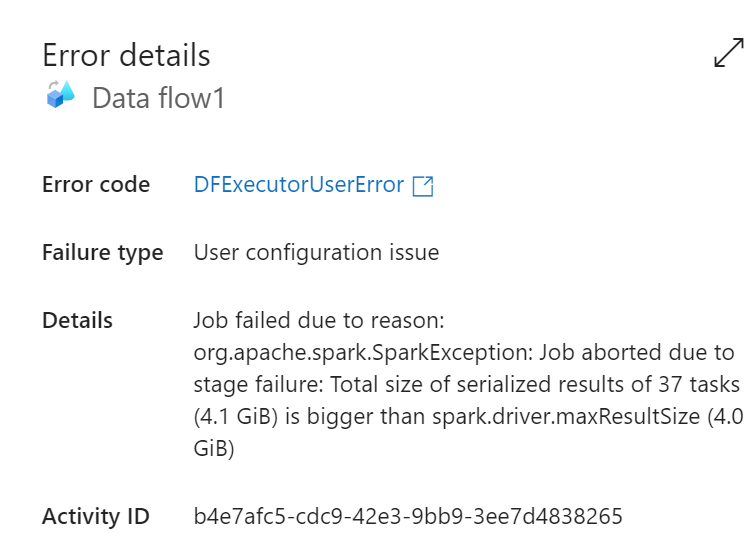
\includegraphics{Img/big.png}

}

\caption{Big Data}

\end{figure}%

\paragraph{Ejemplos de Programas de Big
Data}\label{ejemplos-de-programas-de-big-data}

Uno de los programas más utilizados para manejar Big Data es
\textbf{Apache Hadoop}, una plataforma de código abierto que permite el
procesamiento distribuido de grandes conjuntos de datos a través de
clústeres de computadoras. Hadoop es poderoso, pero requiere una
infraestructura robusta y personal altamente capacitado para su
operación efectiva.

Otro programa clave en el mundo del Big Data es \textbf{Apache Spark},
que se destaca por su velocidad y su capacidad para procesar datos en
tiempo real. Sin embargo, al igual que Hadoop, Spark requiere de una
infraestructura y un equipo de TI que sepa cómo manejarlo, lo que puede
ser un obstáculo para las maquilas que no cuentan con los recursos
necesarios.

\textbf{Tableau} y \textbf{Power BI} son herramientas de visualización
de datos que, aunque no manejan Big Data directamente, permiten a las
empresas interpretar y presentar sus datos de manera más accesible. Sin
embargo, estas herramientas solo son tan buenas como la calidad de los
datos que reciben, lo que significa que, sin una estrategia sólida de
Big Data, su utilidad es limitada.

\begin{figure}[H]

{\centering 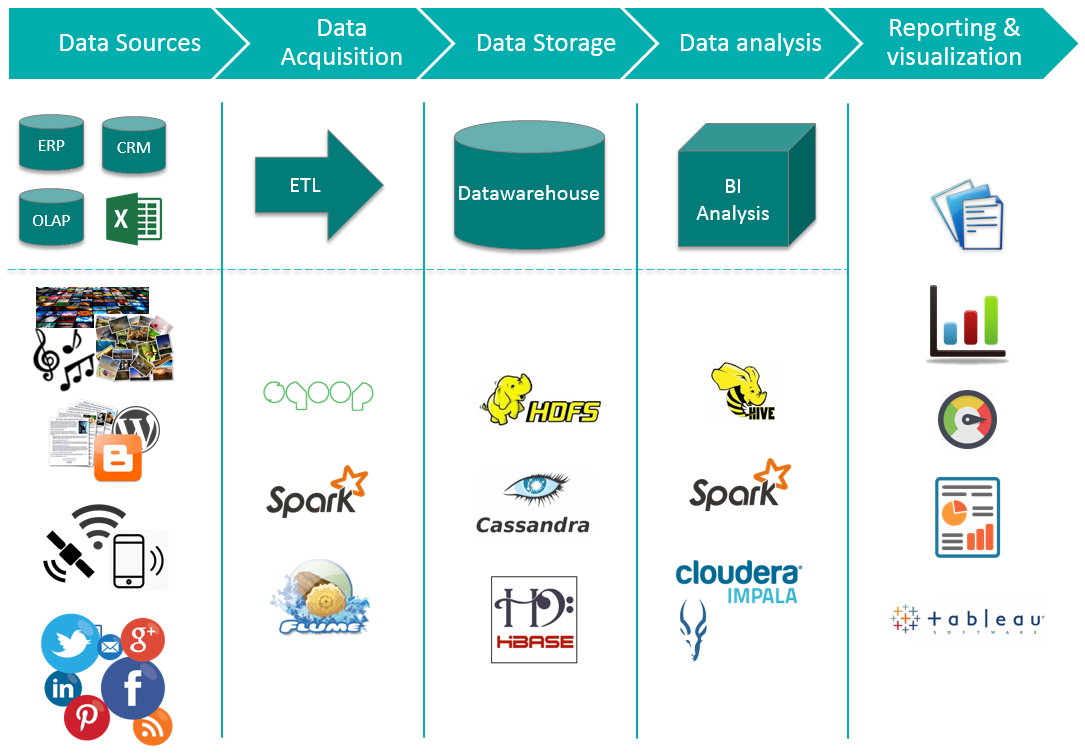
\includegraphics{Img/data.png}

}

\caption{data}

\end{figure}%

\paragraph{Desafíos en el Manejo de Big
Data}\label{desafuxedos-en-el-manejo-de-big-data}

Uno de los principales problemas con Big Data es que muchas maquilas
carecen de la infraestructura adecuada para manejar estos volúmenes
masivos de información. Necesitan servidores potentes, almacenamiento de
datos seguro, y redes rápidas para manejar la transferencia de datos.
Esta infraestructura es costosa y requiere mantenimiento constante, lo
que supone una barrera significativa para las empresas más pequeñas.

Además, el procesamiento y análisis de Big Data requieren personal
altamente capacitado. Los científicos de datos, ingenieros de datos, y
analistas son esenciales para extraer valor de estos datos, pero
encontrar y retener este talento es un reto en sí mismo. A menudo, las
maquilas que intentan implementar estrategias de Big Data se encuentran
con que carecen de los recursos humanos necesarios, lo que lleva a una
subutilización de las herramientas y tecnologías disponibles.

Mientras tanto, en otros países, especialmente en China, el manejo de
Big Data ha sido un foco de inversión masiva. Las empresas chinas han
desarrollado capacidades avanzadas para procesar y analizar grandes
volúmenes de datos, lo que les permite optimizar sus operaciones de
manera que las maquilas de Juárez simplemente no pueden igualar. Esta
brecha tecnológica es preocupante, ya que significa que nuestras
empresas podrían quedarse atrás en un mercado global que cada vez
depende más de la capacidad para manejar y aprovechar los datos.

\subsubsection{Seguridad en la Industria 4.0: Un Riesgo
Constante}\label{seguridad-en-la-industria-4.0-un-riesgo-constante}

La conectividad que trajo la Industria 4.0 ha mejorado mucho la manera
en que trabajamos, pero también ha traído consigo una serie de riesgos
que antes ni imaginábamos. Hoy en día, las maquilas en Juárez están más
expuestas que nunca a ataques cibernéticos. Con todos los sistemas
conectados, desde las máquinas hasta el ERP, cualquier fallo de
seguridad en un punto puede poner en peligro toda la operación.

\paragraph{Ejemplos de Programas de
Seguridad}\label{ejemplos-de-programas-de-seguridad}

En el ámbito de la ciberseguridad, \textbf{Splunk} es uno de los
programas más utilizados para monitorear la seguridad en tiempo real.
Splunk analiza grandes volúmenes de datos y puede detectar
comportamientos anómalos que podrían indicar un ciberataque. Sin
embargo, su implementación y mantenimiento requieren personal capacitado
y una inversión significativa.

\textbf{FireEye} es otra herramienta clave en ciberseguridad, que
proporciona soluciones de detección de amenazas y respuesta rápida ante
incidentes de seguridad. FireEye es potente, pero también caro, lo que
puede ponerlo fuera del alcance de muchas maquilas más pequeñas.

Por otro lado, \textbf{Cisco Umbrella} ofrece seguridad en la nube,
protegiendo a las empresas contra amenazas basadas en internet, como el
phishing y el malware. Aunque es una solución más accesible, también
requiere de una integración adecuada con los sistemas existentes, lo que
puede ser complicado sin el soporte técnico necesario.

\begin{figure}[H]

{\centering 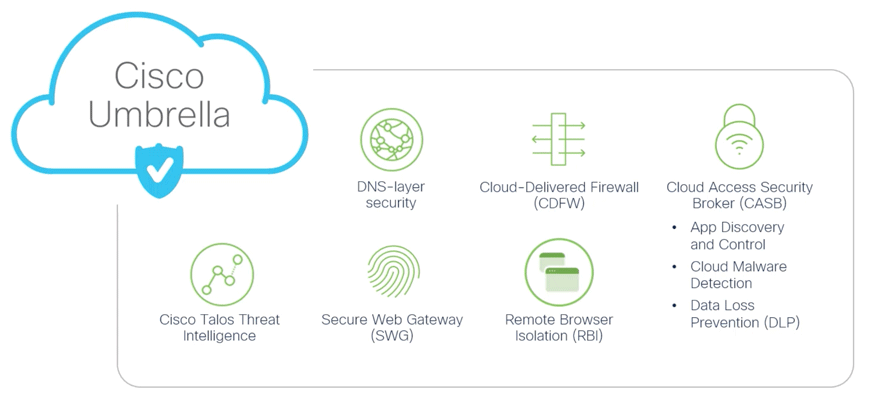
\includegraphics{Img/cisco.png}

}

\caption{umbrella}

\end{figure}%

\paragraph{Desafíos en la
Ciberseguridad}\label{desafuxedos-en-la-ciberseguridad}

Uno de los mayores desafíos en ciberseguridad es mantenerse al día con
las amenazas en constante evolución. Los ciberataques se están volviendo
más sofisticados y frecuentes, y cualquier brecha de seguridad puede
tener consecuencias desastrosas. Para protegerse, las maquilas necesitan
invertir en tecnologías avanzadas y en la formación continua de su
personal, pero esto representa un costo significativo.

Además, la interconexión de todos los sistemas significa que una falla
en un área puede comprometer toda la red. Esto obliga a las empresas a
adoptar un enfoque de seguridad integral, que abarque desde el hardware
hasta el software y los protocolos de usuario. Sin embargo, muchas
maquilas carecen de una estrategia de ciberseguridad bien definida, lo
que las deja vulnerables a ataques que podrían haberse prevenido con
medidas más proactivas.

Mientras tanto, en otras industrias, la ciberseguridad es una prioridad
máxima. En países como China, se han establecido normas estrictas y se
ha invertido mucho en la formación de expertos en seguridad, lo que les
ha permitido proteger mejor sus infraestructuras críticas. Esta
diferencia en el enfoque hacia la ciberseguridad es otro factor que
contribuye a que las maquilas de Juárez se queden atrás en la carrera
por la competitividad global.

\subsubsection{Software Privativo: Un Obstáculo
Inesperado}\label{software-privativo-un-obstuxe1culo-inesperado}

El uso de software privativo es otro de los grandes problemas que
enfrentan las maquilas en la era de la Industria 4.0. Estos sistemas,
aunque poderosos, a menudo imponen restricciones que limitan la
flexibilidad y el control que las empresas tienen sobre sus propios
datos.

\paragraph{Ejemplos de Software
Privativo}\label{ejemplos-de-software-privativo}

\textbf{SAP} es uno de los sistemas ERP más utilizados en la industria
maquiladora, pero es también uno de los más restrictivos en términos de
acceso a los datos. SAP ofrece una gran cantidad de funcionalidades,
pero muchas de ellas están encerradas dentro de su propio ecosistema, lo
que dificulta la integración con otros sistemas o el uso de datos fuera
de su entorno controlado.

\textbf{Oracle} también ofrece soluciones empresariales robustas, pero
al igual que SAP, su enfoque en el software privativo puede limitar la
capacidad de las empresas para utilizar y analizar sus datos de manera
independiente. Las licencias de Oracle son caras, y el software está
diseñado para trabajar dentro de su propio ecosistema, lo que puede ser
una limitación importante para las maquilas que buscan mayor
flexibilidad.

\textbf{Microsoft Dynamics} es otra opción popular, pero también es un
sistema cerrado que impone ciertas restricciones sobre cómo se pueden
utilizar los datos. Aunque Microsoft ofrece una integración más amigable
con otros productos de su suite, sigue siendo un entorno controlado que
puede no ofrecer la libertad que algunas empresas necesitan.

\paragraph{Desafíos del Software
Privativo}\label{desafuxedos-del-software-privativo}

El problema con el software privativo es que, aunque ofrece poderosas
herramientas, también te amarra de manos. Las maquilas que dependen de
estos sistemas se encuentran en una situación en la que no pueden
utilizar sus propios datos fuera del entorno del software, lo que limita
su capacidad para innovar o adaptarse rápidamente a cambios en el
mercado.

Además, la dependencia de un solo proveedor significa que las empresas
están a merced de las decisiones de ese proveedor. Si SAP, Oracle, o
Microsoft deciden cambiar su modelo de negocio, aumentar precios, o
descontinuar soporte para ciertas versiones, las maquilas se encuentran
en una posición difícil, obligadas a seguir la dirección del proveedor o
enfrentarse a costosos procesos de migración.

Esto es particularmente problemático en un entorno de rápida evolución
como la Industria 4.0, donde la flexibilidad y la capacidad de
adaptación son clave para mantenerse competitivo. En contraste, muchas
empresas en China y otros países están adoptando soluciones de código
abierto o desarrollando sus propios sistemas, lo que les da un control
mucho mayor sobre sus datos y procesos. Este enfoque les permite innovar
más rápidamente y adaptarse a los cambios del mercado sin las
restricciones que imponen los sistemas privativos.

\subsubsection{Falta de Talento: Un Talón de
Aquiles}\label{falta-de-talento-un-taluxf3n-de-aquiles}

Sin embargo, el problema más grande al que se enfrenta la Industria 4.0
en Ciudad Juárez es la falta de talento especializado. Mientras que la
tecnología avanza a pasos agigantados, la formación de personal
capacitado no ha seguido el mismo ritmo. Esto ha creado un vacío que es
difícil de llenar, y que está frenando el progreso de muchas maquilas en
su transición hacia la Industria 4.0.

\paragraph{Desafíos en la Generación de
Talento}\label{desafuxedos-en-la-generaciuxf3n-de-talento}

El desafío principal es que la demanda de talento especializado supera
con creces la oferta. Esto significa que las maquilas tienen que
competir no solo entre sí, sino también con empresas de todo el mundo
por los mismos profesionales capacitados. En muchos casos, esto lleva a
una ``guerra de talentos,'' donde las empresas tienen que ofrecer
salarios más altos y beneficios adicionales para atraer y retener a los
expertos que necesitan.

Además, el sistema educativo local no está produciendo el número
suficiente de graduados con las habilidades necesarias. Las
universidades y centros de formación en Ciudad Juárez están tratando de
ponerse al día, pero la brecha entre lo que se enseña y lo que se
necesita en el campo sigue siendo significativa. Esto deja a las
maquilas en una posición difícil, donde tienen que depender de
consultores externos o invertir mucho tiempo y recursos en la
capacitación interna.

En contraste, países como China han hecho de la formación de talento una
prioridad nacional, con programas educativos robustos y alianzas entre
el gobierno, la industria, y las instituciones educativas. Esto les ha
permitido crear un flujo constante de profesionales capacitados listos
para enfrentar los desafíos de la Industria 4.0, mientras que en Juárez
seguimos luchando para llenar las vacantes críticas.

\subsubsection{Atraso vs.~China y Estancamiento en la
Manufactura}\label{atraso-vs.-china-y-estancamiento-en-la-manufactura}

Uno de los efectos más preocupantes de estos desafíos es cómo nos
estamos quedando atrás frente a otras potencias industriales,
especialmente China. Mientras que ellos han integrado la Industria 4.0
en prácticamente todos los aspectos de su economía, nosotros seguimos
rezagados, atrapados en un modelo de maquila tradicional que no termina
de dar el salto hacia la innovación y la creación de valor.

En China, la Industria 4.0 no es solo una tendencia, es una estrategia
de desarrollo nacional. Han invertido millones en tecnología, educación,
y creación de empresas que van mucho más allá de la simple manufactura.
Ellos están liderando en áreas como la inteligencia artificial y la
automatización avanzada, mientras que nosotros seguimos produciendo para
otros, sin desarrollar nuestras propias capacidades tecnológicas.

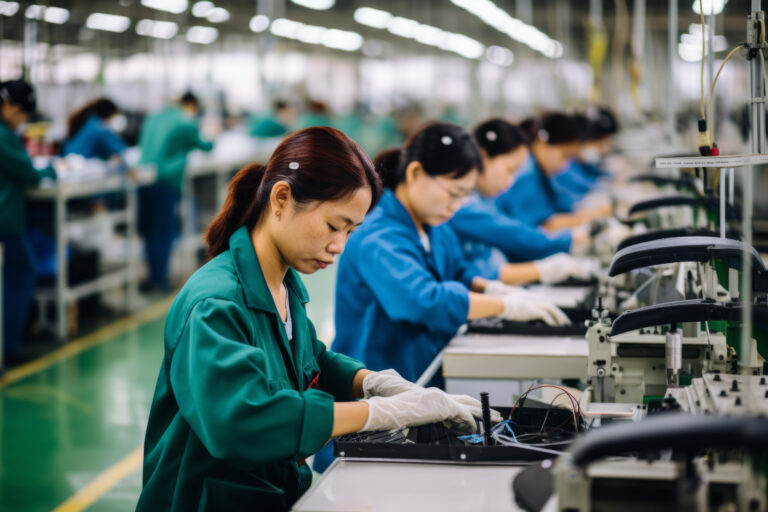
\includegraphics{Img/china.jpg} Este estancamiento nos pone en una
situación vulnerable. Si no tomamos medidas para acelerar la adopción de
la Industria 4.0 y superar estos desafíos, corremos el riesgo de que
nuestras maquilas se queden obsoletas en un mundo que no para de
evolucionar. El desafío es enorme, pero si no lo enfrentamos, podríamos
ver cómo nuestras empresas se quedan atrás, perdiendo competitividad y
relevancia en el mercado global.

\subsection{Reflexión Final}\label{reflexiuxf3n-final}

La Industria 4.0 ofrece una oportunidad increíble para transformar la
industria maquiladora de Ciudad Juárez, pero también nos enfrenta a
retos serios que no podemos ignorar. Si queremos que nuestras empresas
sigan siendo competitivas, necesitamos tomar medidas para superar estos
problemas: mejorar el manejo del Big Data, fortalecer la seguridad,
liberarnos de las limitaciones del software privativo, y, sobre todo,
invertir en la generación de talento especializado.

Es un camino complicado, pero necesario. Si logramos enfrentarnos a
estos desafíos, nuestras maquilas no solo sobrevivirán, sino que podrán
prosperar en un futuro donde la tecnología y la innovación son clave
para el éxito. El tiempo de actuar es ahora, antes de que nos quedemos
completamente rezagados en la carrera industrial global.

\section{Guía Completa para la Adopción Progresiva de la
IA}\label{guuxeda-completa-para-la-adopciuxf3n-progresiva-de-la-ia}

Adoptar la Inteligencia Artificial (IA) en la industria maquiladora es
un reto mayúsculo, pero también una oportunidad que no podemos dejar
pasar si queremos que nuestras maquilas en Ciudad Juárez sigan siendo
competitivas y puedan ponerse al tú por tú con las grandes potencias
industriales del mundo, como China. Sí, es cierto que enfrentamos
desafíos bien duros: la falta de talento especializado, problemas de
ciberseguridad, la dependencia de software privativo que nos ata las
manos con nuestros propios datos, y una cierta sensación de rezago al
compararnos con otras industrias. Pero nada de eso es imposible de
superar. Con un plan bien estructurado, paciencia, y sobre todo con un
compromiso de toda la organización, podemos convertir estos retos en
oportunidades.

Aquí te presento una guía completísima para que, paso a paso, puedas
adoptar la IA en tu maquila de manera gradual, efectiva y sostenible. La
idea no es sólo implementar tecnología por implementarla, sino
transformar tu empresa en una maquila inteligente, capaz de competir en
un mercado global cada vez más exigente.

\begin{quote}
``Implementar estas soluciones requiere una inversión significativa,
tanto en tiempo como en recursos. La realidad es que el mundo no se va a
detener, y si tu maquila no toma las medidas necesarias para adaptarse a
la nueva era tecnológica, te vas a quedar atrás. No solo es una cuestión
de mejora continua, sino de supervivencia. Si no inviertes en modernizar
tu infraestructura, en capacitar a tu equipo, y en adoptar tecnologías
avanzadas como la IA, corres el riesgo de que otra empresa, con un
programa de automatización bien implementado, llegue y te coma el
mandado. Esa empresa podría producir el doble, con menos recursos y a un
costo más bajo, dejándote fuera de la jugada. En un mundo donde la
eficiencia y la innovación son clave, no tomar acción es prácticamente
un boleto directo a la irrelevancia. Así que, aunque el costo inicial
puede parecer alto, la verdad es que no invertir en estas soluciones te
costará mucho más en el largo plazo..''

\begin{itemize}
\tightlist
\item
  \href{https://twitter.com/xavierflorex2}{Javier Flores}
\end{itemize}
\end{quote}

\subsection{Paso 1: Diagnóstico Inicial y Definición de
Objetivos}\label{paso-1-diagnuxf3stico-inicial-y-definiciuxf3n-de-objetivos}

\subsubsection{\texorpdfstring{\textbf{Primero lo Primero: ¿Dónde Estás
Parado?}}{Primero lo Primero: ¿Dónde Estás Parado?}}\label{primero-lo-primero-duxf3nde-estuxe1s-parado}

Antes de lanzarte a meterle IA a tu maquila, lo primero es entender bien
tu punto de partida. No puedes mejorar lo que no conoces, así que hay
que empezar por hacer una radiografía completa de tu empresa: -
\textbf{Infraestructura Tecnológica}: Revisa la tecnología con la que
cuentas actualmente. ¿Tus servidores son lo suficientemente robustos?
¿Tus redes pueden manejar el tráfico de datos que viene con la IA? ¿Tu
almacenamiento es seguro y tiene la capacidad suficiente? Si no tienes
estas bases bien asentadas, cualquier intento de implementar IA podría
quedar en nada. - \textbf{Ciberseguridad}: La seguridad es esencial.
Revisa qué tan protegidos están tus sistemas contra ataques
cibernéticos. ¿Tienes firewalls efectivos? ¿Tus datos están cifrados?
¿Cuentas con un sistema de detección de intrusos? Recuerda que, en la
Industria 4.0, la seguridad no es opcional; es una necesidad. -
\textbf{Talento y Capacidades}: Evalúa el nivel de conocimiento y
habilidades de tu equipo actual en temas relacionados con IA, Big Data,
ciberseguridad, y demás. Identifica dónde hay brechas de conocimiento y
qué habilidades necesitas desarrollar en tu equipo para que puedan
manejar y sacar el máximo provecho de estas nuevas tecnologías.

\subsubsection{\texorpdfstring{\textbf{Definir Objetivos Claros y
Alcanzables}}{Definir Objetivos Claros y Alcanzables}}\label{definir-objetivos-claros-y-alcanzables}

Conocer dónde estás es solo el primer paso. Ahora, tienes que definir
adónde quieres llegar: - \textbf{Corto Plazo (1-2 años)}: Aquí es donde
puedes enfocarte en mejoras rápidas y de impacto inmediato. Por ejemplo,
la automatización de tareas repetitivas que actualmente se hacen de
manera manual en la línea de producción. Esto no sólo te ahorra tiempo,
sino que también reduce errores y aumenta la eficiencia. -
\textbf{Mediano Plazo (3-5 años)}: Una vez que las primeras mejoras
estén funcionando bien, puedes pensar en implementar mantenimiento
predictivo con IA. Esto te permitirá anticiparte a los problemas antes
de que ocurran, evitando paros no programados y extendiendo la vida útil
de tus equipos. - \textbf{Largo Plazo (5-10 años)}: Aquí es donde
empiezas a soñar en grande. Piensa en la integración total de la IA en
todas las operaciones de la maquila, desde la optimización de la cadena
de suministro hasta la automatización de la toma de decisiones
estratégicas. La idea es que tu empresa funcione como un todo
coordinado, con cada parte optimizada y alineada para maximizar la
eficiencia y la productividad.

\begin{figure}[H]

{\centering 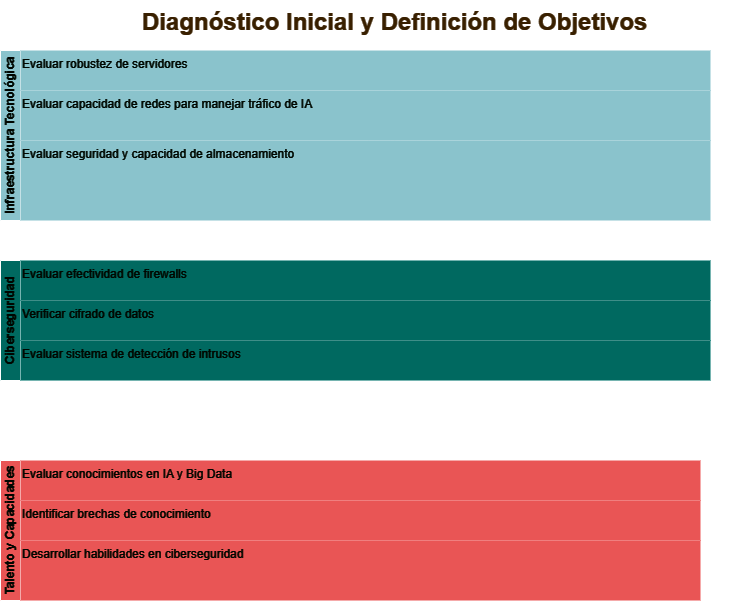
\includegraphics{Img/paso1.png}

}

\caption{Paso 1}

\end{figure}%

\subsection{Paso 2: Mejora la Infraestructura y Desarrolla el
Talento}\label{paso-2-mejora-la-infraestructura-y-desarrolla-el-talento}

\subsubsection{\texorpdfstring{\textbf{Ponte al Día con la
Infraestructura}}{Ponte al Día con la Infraestructura}}\label{ponte-al-duxeda-con-la-infraestructura}

Una vez que tengas claros tus objetivos, es momento de asegurarte de que
tienes la infraestructura necesaria para lograrlos: - \textbf{Actualiza
tus Sistemas}: Si tus servidores ya están viejos o no tienes suficiente
capacidad de almacenamiento, es momento de actualizar. Considera migrar
a soluciones en la nube, como AWS o Google Cloud, que te ofrecen la
escalabilidad y la flexibilidad que necesitas para manejar el incremento
de datos que vendrá con la implementación de IA. - \textbf{Cambia tu
Red}: Si tus redes ya no son eficientes o no tienes suficiente capacidad
de procesamiento, es momento de cambiar. Por ejemplo, puedes mover tus
servidores a una red de datos en la nube. -
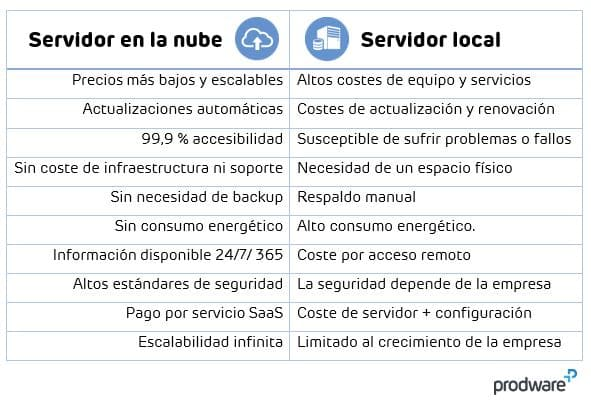
\includegraphics{Img/cloud.jpg}

\begin{itemize}
\tightlist
\item
  \textbf{Fortalece la Seguridad}: La ciberseguridad es una prioridad.
  Invierte en firewalls de última generación, sistemas de detección de
  intrusos, y asegúrate de que todos los datos sensibles estén cifrados
  tanto en tránsito como en reposo. También es vital que establezcas
  protocolos de seguridad claros y que todo tu equipo los entienda y
  cumpla.
\end{itemize}

\subsubsection{\texorpdfstring{\textbf{Capacita a tu Gente: El Talento
es la
Clave}}{Capacita a tu Gente: El Talento es la Clave}}\label{capacita-a-tu-gente-el-talento-es-la-clave}

La tecnología por sí sola no es suficiente; necesitas un equipo
capacitado que sepa cómo manejarla y sacarle el máximo provecho: -
\textbf{Capacitación Interna}: No esperes a que el talento especializado
llegue a tocar tu puerta. Inicia programas de capacitación interna para
que tu equipo actual pueda desarrollar las habilidades necesarias.
Plataformas como \textbf{Coursera}, \textbf{Udemy}, y . \textbf{IA
Center} ofrecen cursos en áreas clave como inteligencia artificial,
análisis de datos, y ciberseguridad. También puedes considerar traer a
expertos para que den talleres o cursos en tu empresa o simplem
networking.

\begin{figure}[H]

{\centering 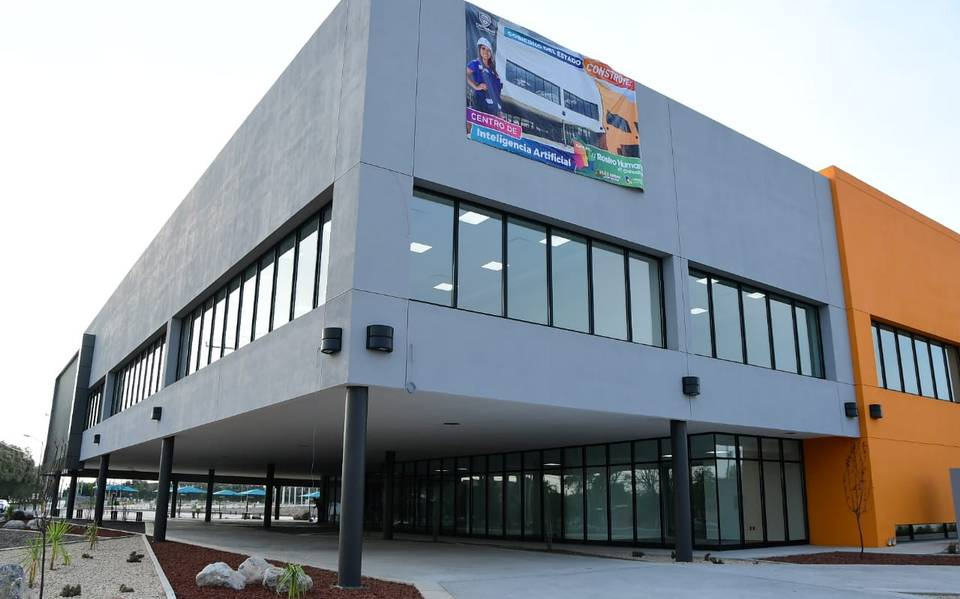
\includegraphics{Img/iacenter.jpeg}

}

\caption{IA Center}

\end{figure}%

\begin{itemize}
\tightlist
\item
  \textbf{Alianzas con Universidades}: Establece relaciones con
  universidades locales y centros de formación técnica para desarrollar
  programas que preparen a los estudiantes específicamente para las
  necesidades de la Industria 4.0 en la maquila. Esto no solo te ayudará
  a formar nuevo talento, sino que también te permitirá atraer a los
  mejores candidatos una vez que estén listos para el mercado laboral.
\end{itemize}

\begin{figure}[H]

{\centering 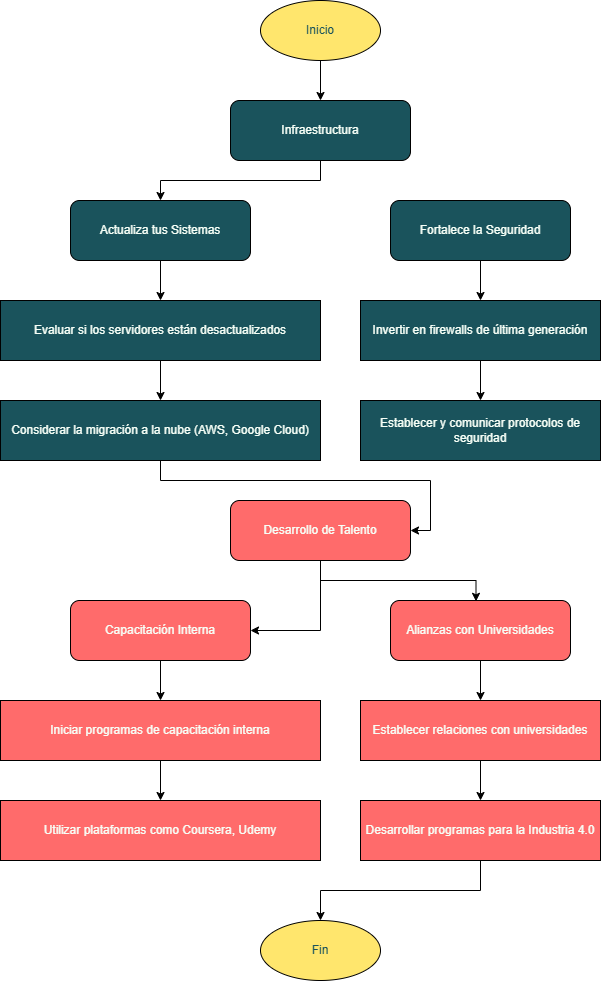
\includegraphics{Img/paso3.png}

}

\caption{Paso 3}

\end{figure}%

\subsection{Paso 3: Implementación Inicial de IA en Áreas
Específicas}\label{paso-3-implementaciuxf3n-inicial-de-ia-en-uxe1reas-especuxedficas}

\subsubsection{\texorpdfstring{\textbf{Paso a Paso: Empieza con
Proyectos
Piloto}}{Paso a Paso: Empieza con Proyectos Piloto}}\label{paso-a-paso-empieza-con-proyectos-piloto}

Transformar toda la maquila de un jalón es como querer correr antes de
aprender a caminar. Es mejor empezar despacio, con proyectos piloto en
áreas clave donde la IA pueda mostrar su valor de manera rápida y clara.
Al hacer esto, no solo reduces el riesgo, sino que también puedes
demostrar a todo el equipo los beneficios tangibles de adoptar esta
tecnología. Aquí te doy algunos ejemplos y recomendaciones para
arrancar:

\begin{itemize}
\item
  \textbf{Selecciona Casos de Uso Específicos}

  Aquí es donde tienes que ponerle coco y pensar en qué partes de tu
  operación necesitan una mejora urgente o dónde la IA puede resolver un
  problema que lleva tiempo molestando. Busca esos puntos críticos donde
  la IA pueda hacer una diferencia real y rápida. Te doy unos ejemplos:

  \begin{itemize}
  \item
    \textbf{Mantenimiento Predictivo}: Imagina poder anticiparte a los
    problemas de tus máquinas antes de que sucedan. Con la IA, puedes
    analizar los datos que generan las máquinas todos los días y
    predecir cuándo es probable que se descompongan. Esto te permite
    hacer el mantenimiento justo a tiempo, antes de que la máquina falle
    por completo, evitando paros inesperados y reduciendo costos de
    reparación. Es como si pudieras ver el futuro y saber cuándo algo va
    a fallar.
  \item
    \textbf{Control de Calidad Automatizado}: Otro gran uso de la IA es
    en el control de calidad. En lugar de revisar manualmente cada
    producto, puedes usar tecnología que inspeccione cada pieza con una
    precisión increíble. Esto no solo acelera el proceso, sino que
    también asegura que todos los productos cumplan con los estándares
    de calidad. Además, reduce el desperdicio porque detecta errores
    antes de que sea demasiado tarde.
  \item
    \textbf{Optimización de Inventarios}: La IA también puede ayudarte a
    manejar mejor tus inventarios. Con herramientas que analizan las
    ventas pasadas y otras variables, puedes predecir cuánto stock
    necesitarás en el futuro, evitando que te quedes corto o que tengas
    exceso de inventario. Así, optimizas tus recursos y ahorras dinero.
  \end{itemize}
\item
  \textbf{Desarrollo de Prototipos de IA}

  No te lances a lo grande sin antes probar las cosas en pequeño.
  Trabaja junto con tu equipo de TI y, si es necesario, colabora con
  expertos externos para desarrollar versiones iniciales (prototipos) de
  las soluciones de IA que quieras implementar. Estos prototipos te
  permiten probar diferentes enfoques sin comprometerte por completo, lo
  que te da la flexibilidad de ajustar y mejorar antes de hacer un
  despliegue más amplio.

  Por ejemplo, si decides probar un sistema de mantenimiento predictivo,
  puedes empezar con una sola máquina o un solo proceso, monitoreando
  cómo se comporta y ajustando la tecnología según sea necesario. Con el
  tiempo, puedes ampliar el uso de la IA a más máquinas o procesos, una
  vez que estés seguro de que todo está funcionando bien.
\end{itemize}

\subsubsection{\texorpdfstring{\textbf{Monitoreo y Ajuste: Perfecciona
sobre la
Marcha}}{Monitoreo y Ajuste: Perfecciona sobre la Marcha}}\label{monitoreo-y-ajuste-perfecciona-sobre-la-marcha}

Implementar IA no es algo que haces una vez y ya está. Necesitas estar
al pendiente de cómo están funcionando los proyectos piloto y hacer
ajustes sobre la marcha para asegurarte de que todo está jalando como
debe:

\begin{itemize}
\item
  \textbf{Pruebas de Rendimiento}

  Después de poner en marcha los proyectos piloto, es esencial que sigas
  de cerca cómo están funcionando. Revisa constantemente si están
  cumpliendo con lo que esperabas: ¿Están reduciendo los costos? ¿Están
  mejorando la eficiencia? ¿Qué tan bien están funcionando las
  predicciones? Estos son los tipos de preguntas que debes hacerte
  mientras monitoreas el rendimiento.

  Si algo no está saliendo como esperabas, no te preocupes; es normal.
  Aquí es donde entra la fase de ajuste. Puede que necesites modificar
  cómo estás usando la IA, cambiar algunos parámetros, o incluso
  reconsiderar el enfoque inicial. Lo importante es que estés dispuesto
  a adaptarte y hacer los cambios necesarios para que los sistemas
  funcionen cada vez mejor.
\item
  \textbf{Retroalimentación Continua}

  No te olvides de hablar con tu equipo. Ellos son los que están usando
  estas nuevas herramientas todos los días y te pueden dar una
  perspectiva valiosa sobre lo que está funcionando y lo que no. Tal vez
  te digan que algunas predicciones no son tan precisas como esperaban,
  o que el sistema es un poco complicado de usar. Escucha sus
  comentarios y usa esa información para hacer ajustes que realmente
  mejoren la operación.

  Hacer esto no solo te ayudará a mejorar la implementación de la IA,
  sino que también hará que tu equipo se sienta involucrado en el
  proceso de cambio, lo que es clave para el éxito a largo plazo.
\end{itemize}

Este paso es crucial porque es donde empiezas a ver los beneficios
reales de la IA, pero también donde te das cuenta de que esto es un
proceso continuo. No se trata solo de instalar la tecnología y esperar
que todo funcione, sino de estar siempre mejorando y ajustando para
obtener los mejores resultados. Si lo haces bien, estos proyectos piloto
se convertirán en la base para una transformación más amplia y profunda
en tu maquila.

\bookmarksetup{startatroot}

\chapter{Casos estudio}\label{casos-estudio}

\section{Soy joto}\label{soy-joto}

\subsection{super mot}\label{super-mot}

\bookmarksetup{startatroot}

\chapter{Aplicaciones de la Inteligencia Artificial en la
Maquiladora}\label{aplicaciones-de-la-inteligencia-artificial-en-la-maquiladora}

\section{El Camino para Adaptar la Inteligencia Artificial en la
Maquiladora}\label{el-camino-para-adaptar-la-inteligencia-artificial-en-la-maquiladora}

La neta es que, hoy en día, la Inteligencia Artificial (IA) ya no es
solo un lujo o una moda; es una necesidad si quieres seguir rifando en
la maquila. En Ciudad Juárez, donde la maquila es el mero corazón
económico, adaptarse a la IA puede hacer la diferencia entre seguir
liderando o quedarte atrás viendo cómo otros te comen el mandado. Pero,
eso sí, hay que ser realistas: meterle IA a la maquila no es tan fácil
como cambiar de máquina o implementar un nuevo software. Es un proceso
que puede ser más o menos complicado, dependiendo de varios factores
como lo técnico, el tiempo que toma, la lana que hay que invertir, y qué
tan listos están tus trabajadores para aceptar el cambio.

Para hacerte la vida más sencilla, hemos desarrollado un \textbf{Ranking
de Adaptación a la IA en la Maquiladora}, que desglosa estos factores
clave para que tengas una mejor idea de qué tan complicado puede ser
para tu maquila subirse al tren de la IA. Con este ranking, podrás
evaluar qué áreas de tu maquila necesitan más atención y qué tanto
esfuerzo te va a costar hacer la transición.

\subsection{Ranking de Adaptación a la
IA}\label{ranking-de-adaptaciuxf3n-a-la-ia}

\begin{enumerate}
\def\labelenumi{\arabic{enumi}.}
\tightlist
\item
  \textbf{Complejidad Técnica}

  \begin{itemize}
  \tightlist
  \item
    \textbf{Alto (5)}: Aquí estamos hablando de cosas que requieren
    conocimientos bien pesados en programación y sistemas complejos.
    Esos proyectos que, si no traes un equipo de TI al cien, te van a
    costar sudor y lágrimas. Ejemplos: Implementar redes neuronales
    profundas para análisis en tiempo real o desarrollar sistemas de
    mantenimiento predictivo que monitoreen un chorro de datos.
  \item
    \textbf{Medio (3)}: Proyectos que ya te piden saberle un poquito a
    la programación, pero que no son una misión imposible. Son cosas que
    implican conectar lo que ya tienes con software de IA, tal vez con
    una que otra personalización. Ejemplos: Usar software de visión por
    computadora para revisar la calidad o meterle chatbots para atender
    a los clientes.
  \item
    \textbf{Bajo (1)}: Aquí estamos hablando de soluciones casi listas
    para usarse, que no te piden saber de códigos ni meterte en broncas
    técnicas. Ejemplos: Plataformas de análisis de datos con IA ya
    configurada o herramientas que te automatizan tareas sencillas.
  \end{itemize}
\item
  \textbf{Tiempo de Implementación}

  \begin{itemize}
  \tightlist
  \item
    \textbf{Largo (5)}: Proyectos que, la neta, van a tomar más de un
    año para completarse. Son esos que necesitan mucho desarrollo a la
    medida, pruebas y que además te piden capacitar a tu gente a fondo.
    Ejemplos: Crear un sistema de IA para manejar toda la cadena de
    suministro.
  \item
    \textbf{Medio (3)}: Implementaciones que te van a tomar entre seis
    meses y un año. No son rápidas, pero tampoco eternas. Ejemplos:
    Meter IA para optimizar inventarios o mejorar la logística interna.
  \item
    \textbf{Corto (1)}: Proyectos que, si le metes ganas, puedes
    terminar en menos de seis meses. Ejemplos: Automatizar tareas
    administrativas o usar IA para predecir ventas.
  \end{itemize}
\item
  \textbf{Inversión Económica}

  \begin{itemize}
  \tightlist
  \item
    \textbf{Alta (5)}: Aquí ya estamos hablando de desembolsar una lana
    considerable. No solo en tecnología, sino también en infraestructura
    y capacitar a tu banda. Ejemplos: Implementar IA en varias áreas de
    producción o comprar robots industriales avanzados con IA.
  \item
    \textbf{Media (3)}: Inversiones más accesibles, donde la lana se
    reparte entre tecnología y capacitación, sin volverte loco.
    Ejemplos: Meter sistemas de mantenimiento predictivo o mejorar el
    control de calidad con visión por computadora.
  \item
    \textbf{Baja (1)}: Proyectos que no te van a dejar en números rojos.
    Tecnología accesible y poca necesidad de cambios grandes. Ejemplos:
    Usar plataformas de análisis de datos con IA o meter asistentes
    virtuales para tareas sencillas.
  \end{itemize}
\item
  \textbf{Capacitación y Adaptación del Personal}

  \begin{itemize}
  \tightlist
  \item
    \textbf{Alta (5)}: Si decides entrarle a algo que requiere un cambio
    radical, prepárate para invertir tiempo y esfuerzo en capacitar a tu
    gente. Aquí la curva de aprendizaje es empinada. Ejemplos: Formar a
    tu equipo en desarrollo de IA, análisis de datos, y gestión de
    proyectos grandes.
  \item
    \textbf{Media (3)}: Capacitación moderada, pero necesaria. Aquí tu
    gente tiene que aprender a usar nuevas herramientas y entender lo
    básico de la IA. Ejemplos: Entrenar al personal en el uso de
    software de control de calidad automatizado o manejar inventarios
    con IA.
  \item
    \textbf{Baja (1)}: Proyectos que no te van a pedir casi nada en
    términos de capacitación. Herramientas fáciles de usar que no
    cambian mucho la forma en que tu banda trabaja. Ejemplos:
    Implementar herramientas de análisis de datos con interfaces
    sencillas o usar chatbots ya preconfigurados.
  \end{itemize}
\item
  \textbf{Impacto en la Cultura Organizacional}

  \begin{itemize}
  \tightlist
  \item
    \textbf{Alto (5)}: Aquí estás hablando de un cambio de raíz en la
    manera de trabajar y gestionar la producción. Es un cambio profundo
    que va a impactar a toda la maquila. Ejemplos: Una transformación
    digital completa que integre IA en todos los niveles de la maquila.
  \item
    \textbf{Medio (3)}: Requiere ajustes en la forma de trabajar, pero
    no cambia la cultura de arriba abajo. Ejemplos: Automatizar procesos
    específicos sin cambiar todo el flujo de trabajo.
  \item
    \textbf{Bajo (1)}: Cambios que tienen un impacto mínimo en la
    cultura de la maquila. Se integran fácilmente en la rutina diaria
    sin mayores broncas. Ejemplos: Usar IA en tareas administrativas o
    para mejoras puntuales en áreas no críticas.
  \end{itemize}
\end{enumerate}

\subsection{Reflexión Final}\label{reflexiuxf3n-final-1}

Este ranking te da un panorama claro de los retos y requisitos que
vienen con la adaptación de la IA en tu maquila. No todas las empresas
están en el mismo punto, y no todas tienen que seguir el mismo camino.
Lo importante es saber dónde estás parado y planificar la transición
para que le saques el máximo jugo a la IA mientras minimizas los
riesgos.

Adoptar la IA no es solo subirse a la ola tecnológica; es una necesidad
para seguir siendo competitivos en un mundo donde la eficiencia, la
precisión, y la capacidad de adaptarse rápido son la clave del éxito. El
camino hacia la IA será diferente para cada maquila, pero con una buena
planificación y una implementación gradual, todas pueden aprovechar los
beneficios que esta tecnología ofrece. ¡Así que a darle con todo,
Juárez!

\section{Aplicaciones de la Inteligencia Artificial en la
Maquiladora}\label{aplicaciones-de-la-inteligencia-artificial-en-la-maquiladora-1}

\section{Machine Learning
Tradicional}\label{machine-learning-tradicional}

La Inteligencia Artificial (IA) ha llegado para cambiar el juego en la
industria maquiladora. Desde la optimización de procesos hasta la
gestión de la cadena de suministro, la IA ofrece un sinfín de
posibilidades para mejorar la eficiencia, reducir costos y elevar la
calidad de los productos. Sin embargo, la implementación de estas
tecnologías puede variar significativamente en términos de complejidad
técnica, tiempo de implementación, inversión necesaria y el impacto en
la cultura organizacional.

En este capítulo, vamos a explorar más a fondo cómo la IA puede ser
aplicada en la maquiladora, desglosando cada área con mayor detalle y
proporcionando un listado de tecnologías clave que pueden ser utilizadas
en cada caso.

\subsection{\texorpdfstring{1. \textbf{Optimización del Proceso de
Producción}}{1. Optimización del Proceso de Producción}}\label{optimizaciuxf3n-del-proceso-de-producciuxf3n}

\textbf{Ranking de Adaptación:} - \textbf{Complejidad Técnica: Alto (5)}
- \textbf{Tiempo de Implementación: Medio (3)} - \textbf{Inversión
Económica: Alta (5)} - \textbf{Capacitación del Personal: Media (3)} -
\textbf{Impacto en la Cultura Organizacional: Alto (5)}

\textbf{Aplicaciones:}

\textbf{a. Mantenimiento Predictivo:}

El mantenimiento predictivo es uno de los usos más poderosos de la IA en
la maquila. Aquí, se utilizan sensores y análisis de datos en tiempo
real para monitorear el estado de las máquinas. La IA analiza estos
datos y predice cuándo una máquina está a punto de fallar, permitiendo
al equipo de mantenimiento actuar antes de que ocurra un problema grave.

\begin{itemize}
\tightlist
\item
  \textbf{Tecnologías Clave:}

  \begin{itemize}
  \tightlist
  \item
    \textbf{Sensores IoT (Internet of Things):} Dispositivos que
    capturan datos como vibración, temperatura, y ruido de las máquinas.
  \item
    \textbf{Plataformas de Machine Learning:} Herramientas como
    \textbf{TensorFlow}, \textbf{PyTorch}, o \textbf{Azure Machine
    Learning} que analizan los datos y hacen predicciones sobre el
    estado de las máquinas.
  \item
    \textbf{Software de Mantenimiento Predictivo:} Soluciones como
    \textbf{IBM Maximo} o \textbf{GE Predix} que integran IA para el
    análisis de datos en tiempo real y la programación de mantenimiento.
  \end{itemize}
\end{itemize}

\textbf{b. Control de Calidad Automatizado:}

El control de calidad es crucial en la maquila, y la IA puede
revolucionar esta área. Con sistemas de visión por computadora y
aprendizaje automático, la IA puede inspeccionar cada producto en la
línea de producción, identificando defectos que serían difíciles de
detectar manualmente.

\begin{itemize}
\tightlist
\item
  \textbf{Tecnologías Clave:}

  \begin{itemize}
  \tightlist
  \item
    \textbf{Cámaras de Visión por Computadora:} Equipos como los de
    \textbf{Cognex} o \textbf{Basler} que capturan imágenes de alta
    resolución de los productos.
  \item
    \textbf{Software de Análisis de Imágenes:} Herramientas como
    \textbf{OpenCV} o \textbf{MATLAB} que procesan las imágenes y
    detectan defectos.
  \item
    \textbf{Redes Neuronales Convolucionales (CNNs):} Algoritmos que
    permiten a la IA reconocer patrones y diferencias sutiles en los
    productos.
  \end{itemize}
\end{itemize}

\textbf{c.~Optimización del Flujo de Trabajo:}

La IA también puede ser utilizada para optimizar el flujo de trabajo en
la maquila. Analizando datos de producción, la IA puede identificar
cuellos de botella y sugerir ajustes en tiempo real para mejorar la
eficiencia.

\begin{itemize}
\tightlist
\item
  \textbf{Tecnologías Clave:}

  \begin{itemize}
  \tightlist
  \item
    \textbf{Sistemas MES (Manufacturing Execution Systems):} Plataformas
    como \textbf{Siemens SIMATIC IT} que integran IA para la gestión del
    flujo de trabajo.
  \item
    \textbf{Análisis de Datos en Tiempo Real:} Herramientas como
    \textbf{Apache Kafka} y \textbf{Elasticsearch} que procesan y
    analizan grandes volúmenes de datos de producción.
  \item
    \textbf{Algoritmos de Optimización:} Uso de técnicas como
    \textbf{Programación Lineal} y \textbf{Algoritmos Genéticos} para
    ajustar el flujo de trabajo y maximizar la eficiencia.
  \end{itemize}
\end{itemize}

\subsection{\texorpdfstring{2. \textbf{Gestión de la Cadena de
Suministro}}{2. Gestión de la Cadena de Suministro}}\label{gestiuxf3n-de-la-cadena-de-suministro}

\textbf{Ranking de Adaptación:} - \textbf{Complejidad Técnica: Medio
(3)} - \textbf{Tiempo de Implementación: Medio (3)} - \textbf{Inversión
Económica: Media (3)} - \textbf{Capacitación del Personal: Baja (1)} -
\textbf{Impacto en la Cultura Organizacional: Medio (3)}

\textbf{Aplicaciones:}

\textbf{a. Optimización de Inventarios:}

La gestión de inventarios es crítica en la maquila. La IA permite
optimizar los niveles de inventario al predecir con precisión la demanda
futura, evitando tanto el exceso como la falta de stock.

\begin{itemize}
\tightlist
\item
  \textbf{Tecnologías Clave:}

  \begin{itemize}
  \tightlist
  \item
    \textbf{Algoritmos de Predicción:} Algoritmos de \textbf{Regresión
    Lineal} y \textbf{Redes Neuronales Recurrentes (RNNs)} que predicen
    la demanda en función de datos históricos.
  \item
    \textbf{Plataformas de Gestión de Inventarios:} Herramientas como
    \textbf{SAP Integrated Business Planning} o \textbf{Oracle SCM
    Cloud} que integran predicciones de IA en la gestión de inventarios.
  \item
    \textbf{Sensores IoT para Inventarios:} Dispositivos que monitorizan
    en tiempo real los niveles de stock en almacenes.
  \end{itemize}
\end{itemize}

\textbf{b. Logística Inteligente:}

La logística es otro campo donde la IA puede hacer maravillas. Con
algoritmos de optimización, la IA puede seleccionar las rutas de
transporte más eficientes, programar envíos y ajustar las operaciones
logísticas en tiempo real.

\begin{itemize}
\tightlist
\item
  \textbf{Tecnologías Clave:}

  \begin{itemize}
  \tightlist
  \item
    \textbf{Algoritmos de Optimización de Rutas:} Herramientas como
    \textbf{Google OR-Tools} que encuentran las rutas más rápidas y
    económicas.
  \item
    \textbf{Sistemas de Gestión de Transporte (TMS):} Plataformas como
    \textbf{Manhattan TMS} o \textbf{JDA TMS} que utilizan IA para
    optimizar la logística y el transporte.
  \item
    \textbf{Plataformas de Análisis Predictivo:} Herramientas como
    \textbf{SAS Predictive Analytics} que analizan datos históricos y
    actuales para optimizar las operaciones logísticas.
  \end{itemize}
\end{itemize}

\subsection{\texorpdfstring{3. \textbf{Automatización de Tareas
Repetitivas}}{3. Automatización de Tareas Repetitivas}}\label{automatizaciuxf3n-de-tareas-repetitivas}

\textbf{Ranking de Adaptación:} - \textbf{Complejidad Técnica: Bajo (1)}
- \textbf{Tiempo de Implementación: Corto (1)} - \textbf{Inversión
Económica: Baja (1)} - \textbf{Capacitación del Personal: Baja (1)} -
\textbf{Impacto en la Cultura Organizacional: Bajo (1)}

\textbf{Aplicaciones:}

\textbf{a. Robots Industriales para Ensamblaje:}

Los robots industriales han estado en la maquila desde hace tiempo, pero
con la IA, estos robots pueden hacer más y mejor. Desde ensamblar
productos hasta empaquetarlos, los robots pueden hacer tareas
repetitivas de manera más rápida y con menos errores que los humanos.

\begin{itemize}
\tightlist
\item
  \textbf{Tecnologías Clave:}

  \begin{itemize}
  \tightlist
  \item
    \textbf{Robots Colaborativos (Cobots):} Equipos como los de
    \textbf{Universal Robots} que trabajan junto a los humanos en la
    línea de producción.
  \item
    \textbf{Sistemas de Control de Robots:} Software como \textbf{ABB
    RobotStudio} o \textbf{Fanuc ROBOGUIDE} que permite programar y
    controlar robots industriales.
  \item
    \textbf{Sensores y Actuadores Inteligentes:} Dispositivos que
    permiten a los robots adaptarse a diferentes tareas y condiciones de
    trabajo.
  \end{itemize}
\end{itemize}

\textbf{b. Automatización de Procesos Administrativos:}

No todas las aplicaciones de la IA tienen que ver con la producción
directa. La IA también puede automatizar tareas administrativas
repetitivas, liberando tiempo para que los empleados se concentren en
actividades más estratégicas.

\begin{itemize}
\tightlist
\item
  \textbf{Tecnologías Clave:}

  \begin{itemize}
  \tightlist
  \item
    \textbf{RPA (Robotic Process Automation):} Herramientas como
    \textbf{UiPath} o \textbf{Blue Prism} que automatizan tareas
    administrativas como la entrada de datos y la generación de
    informes.
  \item
    \textbf{Asistentes Virtuales:} Chatbots y asistentes como
    \textbf{Google Assistant} o \textbf{Microsoft Cortana} que pueden
    manejar tareas básicas de servicio al cliente y administración.
  \item
    \textbf{Software de Gestión Documental:} Plataformas como
    \textbf{DocuWare} que utilizan IA para automatizar la gestión y
    clasificación de documentos.
  \end{itemize}
\end{itemize}

\subsection{\texorpdfstring{4. \textbf{Diseño y Desarrollo de
Productos}}{4. Diseño y Desarrollo de Productos}}\label{diseuxf1o-y-desarrollo-de-productos}

\textbf{Ranking de Adaptación:} - \textbf{Complejidad Técnica: Medio
(3)} - \textbf{Tiempo de Implementación: Medio (3)} - \textbf{Inversión
Económica: Alta (5)} - \textbf{Capacitación del Personal: Media (3)} -
\textbf{Impacto en la Cultura Organizacional: Medio (3)}

\textbf{Aplicaciones:}

\textbf{a. Simulaciones y Pruebas Automatizadas:}

La IA puede acelerar el proceso de diseño y desarrollo de productos al
permitir simulaciones y pruebas automatizadas. Con la IA, puedes
identificar posibles fallos o áreas de mejora antes de que el producto
llegue a la línea de producción.

\begin{itemize}
\tightlist
\item
  \textbf{Tecnologías Clave:}

  \begin{itemize}
  \tightlist
  \item
    \textbf{Software de CAD (Computer-Aided Design):} Herramientas como
    \textbf{AutoCAD} o \textbf{SolidWorks} que integran IA para mejorar
    el diseño de productos.
  \item
    \textbf{Simulación Basada en IA:} Plataformas como \textbf{ANSYS} o
    \textbf{COMSOL Multiphysics} que permiten realizar simulaciones
    complejas antes de fabricar un producto.
  \item
    \textbf{Modelado Predictivo:} Uso de \textbf{Redes Neuronales} y
    \textbf{Algoritmos de Machine Learning} para prever el rendimiento
    del producto bajo diferentes condiciones.
  \end{itemize}
\end{itemize}

\textbf{b. Personalización del Producto:}

La IA también permite personalizar productos según las necesidades del
cliente, adaptando el diseño y la producción para cumplir exactamente
con lo que el mercado demanda.

\begin{itemize}
\tightlist
\item
  \textbf{Tecnologías Clave:}

  \begin{itemize}
  \tightlist
  \item
    \textbf{Configuradores de Producto Basados en IA:} Herramientas que
    permiten a los clientes personalizar productos en línea, integrando
    sus preferencias directamente
  \end{itemize}
\end{itemize}

en la cadena de producción. - \textbf{Software de Fabricación
Personalizada:} Plataformas como \textbf{Tacton} que permiten la
fabricación personalizada basada en configuraciones definidas por el
cliente. - \textbf{Plataformas de Análisis de Mercado:} Herramientas
como \textbf{IBM Watson Marketing} que analizan datos de clientes para
identificar preferencias y tendencias.

\subsection{\texorpdfstring{5. \textbf{Análisis de Mercado y Servicio al
Cliente}}{5. Análisis de Mercado y Servicio al Cliente}}\label{anuxe1lisis-de-mercado-y-servicio-al-cliente}

\textbf{Ranking de Adaptación:} - \textbf{Complejidad Técnica: Bajo (1)}
- \textbf{Tiempo de Implementación: Corto (1)} - \textbf{Inversión
Económica: Baja (1)} - \textbf{Capacitación del Personal: Baja (1)} -
\textbf{Impacto en la Cultura Organizacional: Bajo (1)}

\textbf{Aplicaciones:}

\textbf{a. Análisis Predictivo del Mercado:}

La IA permite analizar enormes cantidades de datos de mercado para
identificar tendencias antes de que se vuelvan obvias. Esto te permite
ajustar tu producción para satisfacer la demanda emergente.

\begin{itemize}
\tightlist
\item
  \textbf{Tecnologías Clave:}

  \begin{itemize}
  \tightlist
  \item
    \textbf{Plataformas de Análisis Predictivo:} Herramientas como
    \textbf{SAS Predictive Analytics} o \textbf{Microsoft Azure Machine
    Learning} que permiten prever las tendencias del mercado.
  \item
    \textbf{Minería de Datos:} Uso de \textbf{Big Data} y
    \textbf{Hadoop} para analizar grandes volúmenes de datos y extraer
    patrones útiles.
  \item
    \textbf{Análisis Sentimental:} Herramientas como \textbf{IBM Watson
    Natural Language Understanding} que analizan el sentimiento del
    cliente en redes sociales y otros canales.
  \end{itemize}
\end{itemize}

\textbf{b. Chatbots y Asistentes Virtuales:}

Los chatbots equipados con IA pueden manejar gran parte de las consultas
de los clientes, resolviendo problemas simples y liberando al personal
para manejar asuntos más complejos.

\begin{itemize}
\tightlist
\item
  \textbf{Tecnologías Clave:}

  \begin{itemize}
  \tightlist
  \item
    \textbf{Plataformas de Chatbots:} Herramientas como
    \textbf{Dialogflow} de Google o \textbf{Microsoft Bot Framework} que
    permiten crear y gestionar chatbots.
  \item
    \textbf{Procesamiento de Lenguaje Natural (NLP):} Tecnologías como
    \textbf{IBM Watson Assistant} que permiten a los chatbots entender y
    responder de manera natural.
  \item
    \textbf{Integración Multicanal:} Soluciones que permiten a los
    chatbots interactuar con los clientes a través de múltiples canales
    como redes sociales, email y mensajería instantánea.
  \end{itemize}
\end{itemize}

\subsection{Conclusión}\label{conclusiuxf3n-1}

La implementación de la IA en la maquiladora no es un proceso de una
sola vez; es una transformación continua que puede llevar a la empresa a
niveles de eficiencia y competitividad sin precedentes. Desde optimizar
procesos de producción hasta mejorar la relación con los clientes, la IA
ofrece un abanico de oportunidades para mejorar cada aspecto del
negocio. Sin embargo, es esencial que cada maquila evalúe sus propias
necesidades y capacidades antes de lanzarse a implementar estas
tecnologías. Con un enfoque planificado y una adaptación gradual,
cualquier maquila puede aprovechar los beneficios de la IA y mantenerse
en la cima de la industria. ¡A darle con todo, Juárez!

\bookmarksetup{startatroot}

\chapter{Impacto Economico}\label{impacto-economico}

\bookmarksetup{startatroot}

\chapter{Futuro}\label{futuro}

\bookmarksetup{startatroot}

\chapter{Recomendaciones}\label{recomendaciones}

\bookmarksetup{startatroot}

\chapter{Summary}\label{summary}

In summary, this book has no content whatsoever.

\bookmarksetup{startatroot}

\chapter*{References}\label{references}
\addcontentsline{toc}{chapter}{References}

\markboth{References}{References}

\phantomsection\label{refs}
\begin{CSLReferences}{0}{1}
\subsection*{Referencias}\label{referencias-1}
\addcontentsline{toc}{subsection}{Referencias}

\begin{enumerate}
\def\labelenumi{\arabic{enumi}.}
\tightlist
\item
  Oscar Martínez, \emph{Ciudad Juárez: El auge de una ciudad fronteriza
  a partir de 1848}, FCE, México, 1982.
\item
  ``La Frontera norte, diagnóstico y perspectivas'', Dirección General
  de Estadística, S.I.C. s/f, mimeo.
\item
  Thomas Madison, \emph{Reseña anual de la industria maquiladora},
  SUGUMEX, México, 1990.
\item
  Bass Zavala, Sonia. ``El crecimiento urbano en Ciudad Juárez,
  1950-2000. Un acercamiento socio-histórico a la evolución desordenada
  de una ciudad de la frontera norte.'' \emph{Chihuahua Hoy} (2013):
  247-289.
\item
  ``La Frontera norte, diagnóstico y perspectivas'', Dirección General
  de Estadística, S.I.C. s/f, mimeo.
\item
  Diario de Juárez, 21 a 24 de agosto de 1981.
\item
  El Fronterizo, 25 de agosto de 1974.
\item
  Guadalupe Ramos, Norte, 9 de febrero de 1994, p.~4A.
\item
  Diario de Juárez, 22 de mayo de 1991.
\item
  Diario de Juárez, 7 de febrero de 1991.
\item
  Declaración de José Manuel Luna, promotor de AMACH, \emph{Novedades},
  20 de enero de 1985.
\item
  Vega, Luis. ``La transformación de la industria maquiladora en la era
  digital.'' \emph{El Financiero}, 2023.
\item
  Secretaría de Economía. ``Informe Anual sobre la Industria
  Maquiladora''. Gobierno de México, 2022.
\end{enumerate}

\end{CSLReferences}


\backmatter

\backmatter
\printbibliography


\end{document}
